
\documentclass[notoc,nofonts,a4paper,twoside,nobib]{tufte-book}
%\documentclass[nofonts,a4paper,twoside]{book}

\usepackage[ngerman]{babel}
\usepackage{currfile,hyperxmp}

\usepackage{filemod}
   \usepackage{dsfont}
\usepackage[
    type={CC},
    modifier={by-sa},
    version={4.0},
    imagewidth = 17mm,
 ]{doclicense}


\usepackage[refsegment=chapter,style=authoryear-comp,natbib=true]{biblatex}

\addbibresource{literature.bib}



\usepackage{amssymb,amsmath}

\usepackage{modiagram}
\usepackage{chemformula}
\usepackage{chemfig}
\renewcommand*\printatom[1]{\ensuremath{\mathsf{#1}}}


\usepackage{tikz}



\newcommand{\inputtikz}[1]{%
%  \tikzsetnextfilename{#1}%
  \input{#1.tikz}%
}


\usetikzlibrary{math,matrix,fit,positioning}

\usetikzlibrary{calc}
\usetikzlibrary{arrows.meta} %needed tikz library

\usepackage{standalone}
\usepackage{pgfplots}
 \pgfplotsset{compat=newest}

\tikzset{>=latex}


\pgfplotsset{
tufte line/.style={
    axis line style={draw opacity=0},
    ytick=\empty,
    axis x line*=bottom,
    x axis line style={
      draw opacity=1,
      gray,
      thick
},
 %   yticklabel=\pgfmathprintnumber{\tick}
  }
  }

\tikzset{
mymat/.style={
    matrix of math nodes,
    left delimiter=|, right delimiter=|,
    align=center,
    column sep=-\pgflinewidth,
}
%,mymats/.style={
%    mymat,
%    nodes={draw,fill=#1}
%} 
 }
 
\newcommand{\myarrow}[5]{\draw[#4](#1.south -| #2)  -- ++(#3 :6mm) node[above,pos=0.55]{$#5$};
} 

\newcommand{\interactLp}[3]{\myarrow{#1-#2-1}{#1.west}{-135}{<-}{#3}} 
\newcommand{\interactLm}[3]{\myarrow{#1-#2-1}{#1.west}{+135}{->}{#3}} 
\newcommand{\interactRp}[3]{\myarrow{#1-#2-2}{#1.east}{ -45}{<-}{#3}} 
\newcommand{\interactRm}[3]{\myarrow{#1-#2-2}{#1.east}{ +45}{->}{#3}}  

\newcommand{\interactout}[2]{\myarrow{#1-1-1}{#1.west}{+135}{->,dashed}{#2}} 

\usetikzlibrary{external}
\tikzexternalize[prefix=tikz_external/]



\usepackage[T1]{fontenc}
\usepackage[utf8]{inputenc}


\usepackage{graphicx}
\setkeys{Gin}{width=\linewidth,totalheight=\textheight,keepaspectratio}


\usepackage{booktabs}
\usepackage{url}
\usepackage{hyperref}

\usepackage{units}

\usepackage{chemformula}

\usepackage{braket}
\setcounter{secnumdepth}{0}

% citations
%\usepackage{natbib}
%\bibliographystyle{plainnat}
%\setcitestyle{round} 

% pandoc syntax highlighting
%\usepackage{color}
%\usepackage{fancyvrb}



% longtable
\usepackage{longtable,booktabs}
\usepackage{multicol}
\usepackage[normalem]{ulem}

% morefloats
\usepackage{morefloats}

\usepackage{calc}


\input{tint_book_header}


\renewcommand{\chaptermark}[1]{\markboth{#1}{}}%


\ifthenelse{\boolean{@tufte@twoside}}
  {\fancyhead[LE]{\thepage\quad{\newlinetospace{Molekülphysik und Festkörperphysik I}}}%
    \fancyhead[RO]{{\newlinetospace{\leftmark}}\quad\thepage}}%
  {\fancyhead[RE,RO]{{\newlinetospace{c}}\quad\thepage}}
  
 
%\makeatletter
\fancypagestyle{mystyle}{%
\fancyhf{}%
\fancyfoot[L]{%
\begin{minipage}{17mm}
\doclicenseImage
\end{minipage}
\begin{minipage}{90mm}
 \footnotesize
 \doclicenseLongText
\end{minipage}%
}% 
%\fancyfoot[L]{\doclicenseThis}% 
}
%\makeatother

\usepackage{etoolbox}
\patchcmd{\chapter}{\thispagestyle{plain}}{\thispagestyle{mystyle}}{}{}



\hypersetup{
 linktocpage,
  colorlinks,
  citecolor=Maroon,
  filecolor=Maroon,
  linkcolor=RoyalBlue,
  urlcolor=RoyalBlue
}

\newcommand{\kapitelname}{Kapitel\ }
\newcommand{\chapterauthors}{Markus Lippitz}
\newcommand{\lastmod}{\Filemodtoday{\currfilepath}}


\newcommand{\addtochapter}{%
\vspace*{-12mm}{
\setlength{\parindent}{0pt}
\chapterauthors \newline \lastmod
}
\vspace*{12mm}
}

\makeatletter
\let\stdchapter\chapter
\renewcommand*\chapter{%
  \@ifstar{\starchapter}{\@dblarg\nostarchapter}}
\newcommand*\starchapter[1]{\stdchapter*{#1}}
\def\nostarchapter[#1]#2{\stdchapter[{#1}]{#2} \addtochapter}
\makeatother

\makeatletter
  \def\my@tag@font{\scriptsize}
  \def\maketag@@@#1{\hbox{\m@th\normalfont\color{gray}\my@tag@font#1}}
  \let\amsmath@eqref\eqref
  \renewcommand\eqref[1]{{\let\my@tag@font\relax\amsmath@eqref{#1}}}
\makeatother

\usepackage[titletoc]{appendix}
\renewcommand{\appendixname}{Anhang}
\renewcommand{\appendixtocname}{Anhang}
\renewcommand{\appendixpagename}{Anhang}

%\includeonly{1_VB/1_VB}
%\includeonly{2_MO/2_MO}
%\includeonly{2_MO/2_MO_teil2}
%\includeonly{3_diel/3_diel}
%\includeonly{4_rot/4_rot}
%\includeonly{5_vib/5_vib}
%\includeonly{6_raman/6_raman}
%\includeonly{7_elec/7_elec}
%\includeonly{8_gitter/8_gitter}
%\includeonly{9_rezi/9_rezi}
%\includeonly{10_phonon/10_phonon}
%\includeonly{11_wk/11_wk}

%\includeonly{anhang/drehimpuls}
%\includeonly{anhang/fourier}


\begin{document}

  \tikzexternaldisable


\title{Experimentalphysik C1 \\ Molekülphysik und Festkörperphysik I}

\author{Markus Lippitz}
\date{\today}


\maketitle


%
\tableofcontents

\renewcommand{\lastmod}{\ \ }
\renewcommand{\chapterauthors}{\ \ }

\chapter*{Vorwort}

Dies ist das Vorlesungsskript meiner Vorlesung 'Molekülphysik und Festkörperphysik I', die ich im zweiten Corona-Semester im Winter 2020/21 gehalten habe. Sie ist eine Kursvorlesung für  Studierende im dritten Jahr des Bachelorstudiums. Bei der Auswahl und Gewichtung der Themen folgt sie sehr stark dem in Bayreuth Üblichen. Ich danke an dieser Stelle insbesondere Jürgen Köhler und Anna Köhler, deren Vorlesungsskripte mir eine große Hilfe waren.


Im Corona-Semester habe ich dieses Skript (nach und nach) an die Studierenden  ausgeteilt. Zu jedem Kapitel gibt es ingesamt circa eine Stunde 'Vorlesung' auf Video, in der ich mündlich durch den Text führe und dabei an den Rand kritzle.
Ich habe den Eindruck, dass es mir beim Sprechen leichter fällt, die Dinge in einen Zusammenhang zu bringen als beim Schreiben, da ich mich traue, schlampiger zu sein. Zur Vorbereitung gab es dann noch ein online multiple-choice Quiz, sowie die Möglichkeit, jederzeit anonym Fragen zu stellen.\sidenote{\href{http://frag.jetzt}{ frag.jetzt}}  In Live-Videokonferenzen besprachen wir offene Fragen und diskutierten Aufgaben ähnlich zu Erik Mazurs 
ConcepTests.\sidenote{\href{https://mazur.harvard.edu/research-areas/peer-instruction}{mazur.harvard.edu}}  Schließlich gab es die in der Physik üblichen Übungszettel und Kleingruppen-Übungen.



Dieses Skript ist 'work in progress', und wahrscheinlich nie wirklich fertig.  Ich danke allen Studierenden des 2020er Jahrgangs, die den Text und die Gleichungen aufmerksam gelesen haben, wodurch wir viele Fehler korrigieren konnten. Trotzdem wird es noch welche geben. Wenn Sie Fehler finden, sagen Sie es mir bitte. 
Die aktuellste Version des Vorlesungsskripts finden Sie auf meiner 
Website.\sidenote{\href{http://www.ep3.uni-bayreuth.de/lecturenotes}{ep3.uni-bayreuth.de}} Dort verlinke ich auch die Videos. Ich habe alles unter eine CC-BY-SA-Lizenz gestellt (siehe Fußzeile). In meinen Worten: Sie können damit machen, was Sie wollen. Wenn Sie Ihre Arbeit der Öffentlichkeit zur Verfügung stellen, erwähnen Sie mich und verwenden Sie eine ähnliche Lizenz. 


Der Text wurde mit der LaTeX-Klasse 'tufte-book' von Bil Kleb, Bill Wood und Kevin Godby\sidenote{\href{https://tufte-latex.github.io/tufte-latex/}{tufte-latex}} gesetzt, die sich der Arbeit von Edward Tufte\sidenote{\href{https://www.edwardtufte.com/}{edwardtufte.com}} annähert. Ich habe viele der Modifikationen angewandt, die von Dirk Eddelbüttel im R-Paket 'tint' eingeführt wurden\sidenote{\href{https://dirk.eddelbuettel.com/code/tint.html}{tint: tint is not Tufte}}. Die Quelle ist vorerst LaTeX, nicht Markdown.




\vspace{2\baselineskip}

Markus Lippitz \\ Bayreuth, 23. Januar 2021

 
 






\part{Theorie der molekularen Bindung}

\renewcommand{\lastmod}{\today}

\chapter{Valenzbindungstheorie}




\section{Ziele}

\begin{itemize}
\item dsf

\item sdvsdfs

\end{itemize}

\section{Überblick}


Die Valenzbindungstheorie (engl. valence bond theory) ist die historisch erste quantenmechanische Theorie zur Molekülbindung. Sie wurde 1927 von
Walter Heitler und Fritz London entwickelt. Kurz darauf entstand die komplementäre Molekülorbitaltheorie, die wir im nächsten Kapitel besprechen werden. Beide Theorien versuchen durch verschiedene Annahmen das quantenmechanische Problem zu lösen, welche Grundzustands-Energie und räumliche Anordnung die vielen Atomkerne und noch viel mehr Elektronen in einem Molekül annehmen.

Die Valenzbindungstheorie (VB) macht die Annahme, dass ein Elektron zunächst einmal zu einem einzigen Atomkern gehört und somit durch ein Atomorbital beschrieben wird. Die Molekülorbitaltheorie (MO) hingegen bildet die Gesamtwellenfunktion aufbauend auf der Annahme, dass jedes Elektron über das gesamte Molekül verteilt ist, also durch Molekülorbitale beschrieben wird. Die Valenzbindungstheorie ist einfacher, insbesondere von Hand, ohne Computer, und führt Begriffe ein, die auch darüber hinaus verwendet werden. Die Molekülorbitaltheorie ist insbesondere durch die Verwendung von Computern weiter entwickelt und 'moderner'.

XXX VB als Paare von Elektronen, Lewis schema ? Bond order ?

Literatur: Atkins: chapter on moleculatr structure
 
\section{Vorbereitung}


\subsection{Orbital oder Wellenfunktion?}

Wir besprechen hier Systeme, die  aus vielen Elektronen bestehen. Die Quantenmechanik und Atomphysik konzentrierte sich jedoch auf das Wasserstoff-Atom mit nur einem Elektron. Wir müssen daher vorsichtig mit der Nomenklatur sein. Die (Gesamt-)Wellenfunktion eines Systems aus $n$ Elektronen ist im allgemeinen Fall $\Psi(\mathbf{r}_1, \mathbf{r}_2, \dots)$, wobei die $\mathbf{r}_i$ die Position des Elektrons $i$ bezeichnen. In dieser Allgemeinheit hängt alles miteinander zusammen und ist viel zu komplex. Wir machen daher immer die Annahme, dass sich die Gesamt-Wellenfunktion als Produkt von Orbitalen $\phi_i$ schreiben lässt
\begin{equation}
\Psi(\mathbf{r}_1, \mathbf{r}_2, \dots) = \phi_1(\mathbf{r}_1) \, \phi_2(\mathbf{r}_2)  \dots
\end{equation}
Die Orbitale hängen also nur von der Position 'ihres' Elektrons ab, nicht von all den anderen Elektronen. Im Fall des Wasserstoff-Atoms mit nur einem Elektron gehen die beiden Begriffe ineinander über.
Diese Aufteilung funktioniert immer, wenn die einzelnen Elektronen nicht miteinander wechselwirken, aber genau das ist der Fall. Diese Näherung versucht also, durch geschickte Wahl der $\phi_i$ diese Wechselwirkung vorweg zu nehmen. Es geht also darum, 'gute' $\phi_i$ zu finden.

\subsection{Born-Oppenheimer Näherung}

Atomkerne sind viel schwerer als Elektronen. In der Born-Oppenheimer Näherung betrachten wir die Kerne als still stehend. Die Elektronen bewegen sich im stationären elektrischen Feld der Kerne. Diese Näherung wird quasi immer gemacht, so dass eigentlich nur erwähnt wird, wenn sie \emph{nicht} eingesetzt wird. Formal bedeutet dies, dass die Wellenfunktion des Moleküls geschrieben werden kann als Produkt der Wellenfunktion aller Elektronen und der Wellenfunktion aller Kerne, also
\begin{equation}
\Psi_{\text{Molekül}}(\mathbf{r}_1, \mathbf{r}_2, \dots, \mathbf{R}_1, \mathbf{R}_2, \dots)
  \approx
  \Psi_{\text{Elektronen}}(\mathbf{r}_1, \mathbf{r}_2, \dots )
\Psi_{\text{Kerne}}( \mathbf{R}_1, \mathbf{R}_2, \dots)
\end{equation}
wobei $\mathbf{r}_i$ Elektronenkoordinaten sind und $\mathbf{R}_i$ Kernkoordinaten.


Wir lösen also die Schrödingergleichung für freie Elektronen-Koordinaten, aber die Kern-Koordinaten werden als fix angenommen. Das \emph{Bindungspotential} stellt die Gesamtenergie des Systems dar, wenn für jeden Punkt der Kurve ein anderer aber jeweils fester Kern--Kern--Abstand angenommen wird.

\section{Das Wasserstoff-Molekül: $\sigma$-Bindung}


Wir betrachten zwei Wasserstoff-Atome $A,B$ mit insgesamt zwei Elektronen $1,2$. Der Hamilton-Operator für ein einzelnes Atom $\hat{H}_A$ ist\sidenote{$r_{ij} = |\mathbf{r}_i - \mathbf{r}_j|$}
\begin{equation}
  \hat{H}_A = - \frac{\hbar^2}{2 m_1} \nabla_1^2 - \frac{e^2}{4 \pi \epsilon_0} \frac{1}{r_{A1}}
\end{equation}
Die Wellenfunktion $\phi_A(\mathbf{r_1})$ löst damit die Schrödinger-Gleichung. Zwei sehr weit voneinander entfernte Wasserstoff-Atome haben die Gesamt-Wellenfunktion
\begin{equation}
 \Psi = \phi_A(\mathbf{r}_1) \, \phi_B(\mathbf{r}_2)
\end{equation}
Wenn die beiden Atome nahe beieinander sind, kann man nicht mehr sagen, ob Elektron $1$ bei Kern $A$ oder Kern $B$ ist. In dieser Situation ist daher die Gesamt-Wellenfunktion 
\begin{equation}
 \Psi = \phi_A(\mathbf{r}_2) \, \phi_B(\mathbf{r}_1)
\end{equation}
genauso gut möglich. In der Quantenmechanik löst man dies auf durch die Superpostion der beiden Möglichkeiten. Die Gesamt-Wellenfunktion  ist daher 
\begin{equation}
 \Psi_{\pm} = \phi_A(\mathbf{r}_1) \, \phi_B(\mathbf{r}_2) \, \pm \, \phi_A(\mathbf{r}_2) \, \phi_B(\mathbf{r}_1)
\end{equation}
Dies löst die Schrödinger-Gleichung mit dem Gesamt-Hamilton-Operator
\begin{equation}
  \hat{H}_{ges} =  \hat{H}_A + \hat{H}_A  + \frac{e^2}{4 \pi \epsilon_0} \left( \frac{1}{r_{12}} + \frac{1}{r_{AB}} \right)
\end{equation}
wobei der Term mit $r_{AB}$ auch zunächst weggelassen werden kann, weil die Kern-Positionen in der Born-Oppenheimer-Näherung ja als konstant angenommen werden.

Es zeigt sich\sidenote{Rechnung in Haken / Wolf II, Kapitel 4.4.2}, dass die symmetrische Superposition die niedrigere Gesamtenergie liefert. Die beiden Terme der Wellenfunktion interferieren konstruktiv und sorgen dafür, dass im Raum zwischen den beiden Kernen eine höhere Aufenthaltswahrscheinlichkeit der Elektronen zu finden ist. Diese kompensiert die Coulomb-Abstoßung der Kerne.

In der Valenzbindungstheorie entstehen Bindungen zwischen Atomen durch das 
Paaren von zwei Elektronen. Zwei Kerne teilen sich also zwei Elektronen, die nicht mehr einem einzelnen Kern zugeordnet sind.

Der Spin der beteiligten Elektronen muss anti-symmetrisch gegen Vertauschung sein, da die Ortswellenfunktion ja symmetrisch ist, und das Pauli-Prinzip eine insgesamt anti-symmetrische Wellenfunktion  verlangt.

Die Ortswellenfunktion des Orbitals $\Psi_{+}$ ist wechselt nicht das Vorzeichen bei Rotation um die Kern--Kern--Achse. Dies ist analog zum s-Orbital im Wasserstoff-Atom bei Rotation um die (willkürlich gewählte oder durch das Magnetfeld gegebene) z-Achse.  Diese Bindung wird daher als \emph{$\sigma$-Bindung} bezeichnet. In beiden Fällen besitzt das Elektron keinen Drehimpuls.




\section{Die $\pi$-Bindung}

Die Art der Bindung hängt von der Orientierung der beteiligten Orbitale zueinander ab. Als Beispiel betrachte wir das Molekül N$_2$. Die Elektronenkonfiguration von Stickstoff ist [He]2s$^2$2p$_x^1$2p$_y^1$2p$_z^1$. Wir nehmen die z-Achse als Verbindungsachse der Kerne. Hier zeigen zwei p$_z$-Orbitale aufeinander. Eine $\sigma$-Bindung entsteht durch Paarung der beiden einzelnen Elektronen in den  p$_z$-Orbitalen, da die resultierende Wellenfunktion wieder rotationssymmetrisch um die Verbindungsachse sein wird. Sie hat die gleiche symmetrische Form wie oben.

Aus den p$_x$ und p$_y$-Orbitalen erhält man je eine $\pi$-Bindung: Die hantelförmigen p-Orbitale liegen parallel zueinander und senkrecht zur Bindungsachse. Dabei überlappen im Gegensatz zur $\sigma$-Bindung der p$_z$-Orbitalen beide Teile der Hanteln. Das Elektron in diesem bindenden Orbital hat einen Drehimpuls von $1 \hbar$ entlang der Kern--Kern--Achse, daher wird dies $\pi$-Bindung genannt.


Insgesamt ist N$_2$ also aus einer $\sigma$-Bindung und zwei $\pi$-Bindungen
aufgebaut.


\section{Bindungswinkel}

Wenn drei oder mehr Atome ein Molekül bilden, dann kann man den Winkel einer Bindung definieren und oft aus der Valenzbindungstheorie (näherungsweise) vorhersagen. Als Beispiel betrachten wir H$_2$O. Die Elektronenkonfiguration von Sauerstoff ist [He]2s$^2$2p$_x^2$2p$_y^1$2p$_z^1$. Für die Bindung relevant sind die ungepaarten Elektronen in den hier p$_y$ und p$_z$ genannten Orbitalen. Diese gehen jeweils eine $\sigma$-Bindung mit dem 1s-Elektron des Wasserstoffs ein. Das p$_y$-Orbital steht senkrecht auf dem  p$_z$-Orbital von Sauerstoff. Daher erwarten wir einen Bindungswinkel von 90$^\circ$. Dies ist nahe aber nicht exakt am experimentellen Wert von 104.5$^\circ$.


\section{Hybridisierung}

Insbesondere in der organischen Chemie der Kohlenwasserstoffe spielt die Hybridisierung der Kohlenstoff-Orbitale eine wichtige Rolle. Im Kohlenstoff-Atom besteht nur ein geringer Energieunterschied zwischen der energetisch niedrigsten Elektronenkonfiguration
[He]2s$^2$2p$_x^1$2p$_y^1$2p$_z^0$ und der nächst höheren [He]2s$^1$2p$_x^1$2p$_y^1$2p$_z^1$. Dies bedeutet, dass der Energieunterschied zwischen dem 2s und dem 2p-Orbital in Kohlenstoff sehr gering ist, und insbesondere 
ist der Energiegewinn durch die Bindung sehr oft größer als dieser Unterschied. Es ist daher oft energetisch günstiger, die Bindung ausgehend von einer Linearkombination von 2s und 2p-Orbitalen zu betrachten. Dies nennt man Hybridisierung der Orbitale. Wenn ein s-Orbital und drei p-Orbitale beteiligt sind, dann wird dies als sp$^3$-Hybridisierung bezeichnet. Ohne Hybridisierung könnte Kohlenstoff nur zwei Bindungen eingehen (mit den p$_x$ und p$_y$-Orbitalen), nach sp$^3$-Hybridisierung vier, so dass die Gesamtenergie stärker abgesenkt werden kann.\sidenote{Auch ist die Idee eines s- oder p-Orbitals ein Ein-Elektron-Konzept, das in Mehrelektronen-Atomen durch die anderen Elektronen gestört wird.}

Die neuen Hybrid-Orbitale $h_{1 .. 4}$ sind so gewählt, dass $\braket{h_i | h_j} = \delta_{ij}$, also
\begin{eqnarray}
 h_1 = s + p_x + p_y + p_z \\
 h_2 = s + p_x - p_y - p_z \\
 h_3 = s - p_x + p_y - p_z \\
 h_4 = s - p_x - p_y + p_z 
\end{eqnarray}
Diese Orbitale entstehen also durch Interferenz der ursprünglichen Orbitale und haben eine Ladungsverteilung, deren Keulen einen Tetraeder aufspannen. Der Bindungswinkel ist $\arccos (-\frac{1}{3}) = 109.5^\circ$. Methan (CH$_4$) ist daher tetraederförmig.

Analog gibt es auch die sp$^2$ und die sp-Hybridisierung.  Die sp$^2$-Hybridisierung findet man beispielsweise in Ethen (C$_2$H$_4$). Die drei  sp$^2$-Orbitale jedes Kohlenstoff-Atoms sind an der Bindung der beiden Wasserstoff-Atome beteiligt und an einer der beiden C--C Bindungen. Die zweite C--C Bindung ist eine 'gewöhnliche' $\sigma$-Bindung zwischen den verbleibenden, nicht hybridisierten p-Orbitalen. Dadurch ergeben sich die Winkel in der HCH bzw. HCC-Bindung zu circa 120$^\circ$.

Ein Beispiel für die sp-Hybridisierung ist Ethin (C$_2$H$_2$).


\section{Bezeichnung von Molekülzuständen}

siehe demtröder chap. 2.4.3

In der Atomphysik gibt es für jedes Elektron die Quantenzahlen $n$, $l$, $m_l$, $s$, $m_s$, $j$, $m_j$, die (bis auf $n$) die Länge und die Orientierung eines Drehimpuls-artigen Vektors anzeigen. Die Größe des Bahndrehimpulses, also die 
Quantenzahl $l$ wird als s,p,d,f, ... angegeben. In Mehrelektronen-Atomen bildet man vektorielle Summen über die einzelnen Vektoren der Elektronen. Je nach Kopplungsschema addiert man zunächst alle Bahndrehimpulse $\vec{l}$ und Spins $\vec{s}$, oder alle Gesamtdrehimpulse $\vec{j}$. Das Ergebnis wird dann wieder als Längen- und Orientierungsquantenzahl angegeben, also $L$, $M_L$, $S$, $M_S$, $J$ und $M_J$.





Der wichtigste Unterschied in Molekülen ist, dass die Vorzugsrichtung oder z-Achse durch die Kern--Kern--Achse immer gegeben ist. Da Drehimpulserhaltung Rotationssymmetrie voraussetzt, ist in Molekülen nur noch die Drehimpuls-Komponenten entlang der Kern--Kern--Achse eine gute Quantenzahl. $m_l$ übernimmt also die Rolle von $l$ in der Atomphysik. Manchmal wird $l$ noch angegeben, sagt dann aber nur noch aus, in welcher Quantenzahl $l$ das Elektron landen würde, wenn das Molekül zu einzelnen Atomen auseinandergezogen würde.

Weiterhin hängt die Gesamtenergie nicht vom Vorzeichen von $m_l$ ab, so dass $\lambda = | m_l | $ eingeführt wird. Analog zu $l$ in der Atomphysik wird der Wert von $\lambda$ als $\sigma, \pi, \delta, \phi, \dots$ dargestellt, wie wir es bei der Klassifizierung der Bindungen schon gesehen hatten.\sidenote{Anti-bindenden Orbitale werden dabei mit einem hochgestellten Stern gekennzeichnet, beispielsweise $\pi^\star$.} Man beachte jedoch, dass somit alle Zustände außer $\lambda = 0$ zweifach entartet sind, da ja $m_l = \pm \lambda$.


Analog zum Mehrelektronen-Atom können im Molekül auch Gesamt-Quantenzahlen definiert werden. Wie im Atom auch sind die Projektionen auf die Achse einfach per Addition zu gewinnen:
\begin{equation}
M_S = \sum m_s{_i} \quad \text{und} \quad M_L  = \sum m_{l_i}
\end{equation}
Wie beim einzelnen Elektron ist auch wieder $\Lambda = | M_L|$ die interessantere Größe, die ebenfalls wieder als $\Sigma, \Pi, \Delta, \Phi, \dots$ dargestellt wird. Wenn die Länge des Gesamt-Spin-Vektors $|\vec{S}| = \hbar \sqrt{S (S+1)}$ ist, dann muss  $M_S$ ist zwischen $-S$ und $S$ liegen, kann also  $2S + 1$  verschiedene Werte annehmen.\sidenote{Daher Triplett für $S=1$ und Singulett für $S=0$.} Dies wird als Multiplizität bezeichnet. Für den Gesamt-Drehimpuls $\vec{J}$ ist analog auch nur der Betrag der Projektions-Komponenten interessant, die $\Omega$ genannt wird
\begin{equation}
 \Omega = | M_J | = | \Lambda + M_S|
\end{equation}
Dies alles wird zum spektroskopischen Termsymbol zusammengefasst:
\begin{equation}
 ^{2 S + 1}\Lambda_\Omega
\end{equation}


https://chemistry.stackexchange.com/questions/67031/determination-of-reflections-in-sigma-molecular-term-symbols


\printbibliography[segment=\therefsegment,heading=subbibliography]


\renewcommand{\lastmod}{April 29, 2020}

\chapter{Molekülorbitaltheorie}




\section{Ziele}

\begin{itemize}
\item dsf

\item sdvsdfs

\end{itemize}

\section{Überblick}

Die Molekülorbitaltheorie  (MO) baut zunächst neue (Ein-Elektron-) Orbitale, die sich über das ganze Molekül erstrecken. Dann werden in diese Orbitzale nach und nach Elektronen eingefüllt, analog zu Mehr-Elektronen-Atomen in der Atomphysik. Dabei wird die Wechselwirkung zwischen den Elektronen zunächst vernachlässigt. Die MO-Theorie macht also andere Näherungen als die Valenzbindungstheorie.


\section{Vorbereitung}

\subsection{Störungsrechnung}

\subsection{Variationsprinzip}

Wir schreiben die Schrödinger-Gleichung
\begin{equation}
 \hat{H} \ket{\Psi} = E \, \ket{\Psi} 
\end{equation}
um durch Multiplikation von links mit $\bra{\Psi}$ und erhalten
\begin{equation}
 E = \frac{\braket{\Psi | H | \Psi}} {\braket{\Psi | \Psi}}
 \label{eq:MO_variation}
\end{equation}
Den Term auf der rechten Seite kann man für beliebige Wellenfunktionen ausrechnen. Die Mathematik sagt aber, dass er minimal wird, wenn die Wellenfunktion eine Eigenfunktion von $\hat{H}$ ist, also die Schrödinger-Gleichung erfüllt. Wir probieren nun also verschiedene Test-Funktionen durch und versuchen, die Energie nach Gl.~\ref{eq:MO_variation} zu minimieren. Dadurch nähern wir uns der echten Eigenfunktion immer mehr an, die Lösung der Schrödinger-Gleichung ist.

Sei die Testfunktion
\begin{equation}
 \ket{\Psi} = c_1 \ket{\phi_1} + c_2 \ket{\phi_2}
\end{equation}
mit normierten  $\ket{\phi_i}$ und reell-wertigen Koeffizienten $c_i$. Damit erhält man
\begin{eqnarray}
\braket{\Psi | \Psi}  &= & c_1^2 + c_2^2  + 2 c_1 c_2 \underbrace{\braket{\phi_1 | \phi_2}}_{= S}\\
\braket{\Psi |  H | \Psi} &=& c_1^2 \underbrace{\braket{\phi_1 |  H | \phi_1 }}_{= H_{11}} +
										c_2^2 \underbrace{\braket{\phi_2 |  H | \phi_2 }}_{= H_{22}} +
								2 c_1 c_2 \underbrace{\braket{\phi_1 |  H | \phi_2 }}_{= H_{12}} 
\end{eqnarray}
Dabei bezeichnet $S$ das Überlapp-Integral der beiden Wellenfunktionen, und $H_{ij}$ die Matrix-Elemente des Hamilton-Operators. Die Diagonalelemente $H_{11}$ und $H_{22}$ geben die Coulomb-Energie an, die Außerdiagnoalelemente $H_{12} = H_{21}$ die Austausch-Energie. Mit diesen Abkürzungen kann man die Eigen-Energie schreiben als
\begin{equation}
  E = \frac{c_1^2 H_{11} + c_2^2 H_{22} + 2 c_1 c_2 H_{12}}{c_1^2 + c_2^2 + 2 c_1 c_2 S}
\end{equation}
Für eine minimale Eigenen-Energie $E$ müssen die partiellen Ableitungen nach $c_i$ beide Null sein, oder
\begin{equation}
 \begin{vmatrix}
   H_{11} - E & H_{12} - E \, S \\  H_{12} - E \, S & H_{22} - E \\
 \end{vmatrix}
= 0
\quad
\text{oder} \quad
E_\pm = \frac{H_{11} \pm H_{12}}{1 \pm S}
\end{equation}
wobei wir im letzten Schritt angenommen haben, dass $H_{11} = H_{22}$.

\section{Das Wasserstoff-Molekül-Ion H$_2^+$}

Als Beispiel für das Variationsprinzip in der Molekülorbitaltheorie betrachten wir das Wasserstoff-Molekül-Ion\sidenote{Dies wäre auch exakt möglich, mittels elliptischer Koordinaten, siehe z.B. Demtröder, Molekülphysik Kap. 2.4.1} H$_2^+$. Es gibt also nur ein Elektron, was das Problem der Elektron-Elektron-Wechselwirkung umgeht.

Wir benutzen wie immer die Born-Oppenheimer-Näherung. Die Kerne bewegen sich also nicht und tragen somit auch nicht zur kinetischen Energie bei. Der Abstand des einzigen Elektrons zu den beiden Kernen sei $r_1$ und $r_2$. Der Hamilton-Operator des Gesamtsystems ist
\begin{equation}
\hat{H} =  - \frac{\hbar^2}{2 m} \nabla^2 - \frac{e^2}{4 \pi \epsilon_0} \frac{1}{r_{1}} - \frac{e^2}{4 \pi \epsilon_0} \frac{1}{r_{2}}
= \hat{H}_1  - \frac{e^2}{4 \pi \epsilon_0} \frac{1}{r_{2}}
\end{equation} 
wobei $\hat{H}_1 $ der Hamilton-Operator des Wasserstoff-\emph{Atoms} ist. Die Coulomb-Energie der beiden Kerne untereinander hängt nur vom Kern--Kern--Anstand ab und ist somit eine Konstante, die später zur Gesamtenergie addiert werden wird.

Wir suchen Molekül-Orbitale $\ket{\Psi}$, die mit $\hat{H}$ die Schrödinger-Gleichung lösen, und kennen bereits die Lösungen für $\hat{H}_1$:
\begin{equation}
\hat{H} \ket{\Psi} = E \ket{\Psi} \quad \text{und} \quad 
\hat{H}_1 \ket{\phi} = E_1 \ket{\phi} 
\end{equation}
Da die beiden Kerne identisch sind, gibt es solche Lösungen $\ket{\phi_2}$ in der gleichen Form aber zentriert um eine andere Kernposition auch für den zweiten Kern. Linearkombinationen von diesen  $\ket{\phi_{1,2}}$ nehmen wir jetzt als Testfunktion $\ket{\Psi}$. Dies nennt man \emph{linear combination of atomic orbitals} (LCAO).

Wir folgen dem oben dargestellten Variationsprinzip und müssen nur die drei Integrale $S$, $ H_{11}$ und $H_{12}$ diskutieren.

\paragraph{Überlappintegral $S$} Das Integral $S$ beschreibt den räumlichen Überlapp der beiden Atom-Wellenfunktionen, wenn die einen um Kern 1, die andere um Kern 2 zentriert ist:
\begin{equation}
 S = \braket{\phi_1 | \phi_2} = \int \phi_1( \mathbf{r} - \mathbf{r}_1)  \, \phi_2( \mathbf{r} - \mathbf{r}_2)   \, d\mathbf{r}
\end{equation}
Dabei bezeichnet $\mathbf{r}$ die Position des Elektrons und  $\mathbf{r}_{1,2}$  die Position der Kerne.\sidenote{Wasserstoff-Wellenfunktionen sind reell-wertig.} Da die $\ket{\phi}$ normiert sind, liegt der Wert von $S$ zwischen $0$ und $1$.

\paragraph{Coulomb-Wechselwirkung $H_{11}$}  Dieser Term beschreibt die Coulomb-Energie des Elektrons in der atomaren Wellenfunktion $\phi_1$, aber in Gegenwart beider Kerne:
\begin{eqnarray}
H_{11} &= &  \braket{\phi_1 | \hat{H} | \phi_1} = \braket{\phi_1 | \hat{H}_1 | \phi_1}  - \braket{\phi_1 |  \frac{e^2}{4 \pi \epsilon_0} \frac{1}{r_{2}} | \phi_1}  \\
 & = & E_1 - \frac{e^2}{4 \pi \epsilon_0} \int \frac{|\phi_1(\mathbf{r})|^2 }{|\mathbf{r} - \mathbf{r}_2  |} \, d\mathbf{r} = E_1 + C
\end{eqnarray}
Das Ergebnis ist die Eigen-Energie des Elektrons im Wasserstoff-\emph{Atom}, korrigiert im ein Überlappintegral der Ladungsdichte ${|\phi_1(\mathbf{r})|^2 }$ um den einen Kern im Coulomb-Potential des anderen Kerns. Der Korrekturterm $C$ ist negativ.

\paragraph{Austausch-Wechselwirkung $H_{11}$} Die Austausch-Wechselwirkung ist ein rein quantenmechanischer Effekt.
\begin{eqnarray}
H_{12} &= &  \braket{\phi_1 | \hat{H} | \phi_2} = \braket{\phi_1 | \hat{H}_1 | \phi_2}  - \braket{\phi_1 |  \frac{e^2}{4 \pi \epsilon_0} \frac{1}{r_{2}} | \phi_2}  \\
 & = & E_1 \, S - \frac{e^2}{4 \pi \epsilon_0} \int \frac{ \phi_1(\mathbf{r}) \, \phi_2(\mathbf{r})  }{|\mathbf{r} - \mathbf{r}_2  |} \, d\mathbf{r} = E_1 \, S + A
\end{eqnarray}
Die Austausch-Dichte $\phi_1(\mathbf{r}) \, \phi_2(\mathbf{r})$ ist ähnlich einer Ladungsdichte $|\phi(\mathbf{r})|^2$, nur dass zwei verschiedenen Wellenfunktionen eingehen. Das Elektron wechselt sozusagen zwischen der Zugehörigkeit zu Kern 1 und 2. Der Korrekturterm $A$ ist ebenfalls negativ.

Mit diesen Integralen wird die Gesamtenergie
\begin{equation}
E_\pm = \frac{H_{11} \pm H_{12}}{1 \pm S} = E_1 + \frac{C \pm A}{1 \pm S}
\end{equation}
Die zugehörigen Molekül-Orbitale sind die symmetrische und die anti-symmetrisch Kombination der Atom-Orbitale
\begin{equation}
\ket{\Psi_\pm }= \frac{1}{\sqrt{2 (1 \pm  S)}} \, \left( \ket{\phi_1} \pm \ket{\phi_2} \right)
\end{equation}

Zur Berechnung der Bindungsenergie nehmen wir jetzt die nur vom Kern--Kern--Abstand $R$ abhängende Coulomb-Energie der Kerne wieder hinzu
\begin{eqnarray}
 E_\text{Bindung} &=&  E_\text{Molekül} -  E_\text{Atom} \\
  &=&   E_1 + \frac{C \pm A}{1 \pm S} + \frac{e^2}{4 \pi \epsilon_0} \frac{1}{R} - E_1 \\
   &=&\frac{C }{1 \pm S}  + \frac{e^2}{4 \pi \epsilon_0} \frac{1}{R}  \pm \frac{ A}{1 \pm S}  \label{eq:MO_E_bindung_h2p}
\end{eqnarray}
Numerische Rechnungen zeigen, dass das Überlapp-Integral $S$ keinen Entscheidenden Einfluss auf das Ergebnis hat, wir es hier also nicht weiter betrachten müssen.

Das Coulomb-Integral $C$ ist für einen  großen Kern--Kern--Abstand $R$ quasi die Energie einer Punkt-Ladung im Potential des anderen Kerns, da die Ausdehnung der Wellenfunktion $\phi_1$ vernachlässigt werden kann. Da $C$ negativ ist, kompensieren sich dann die ersten beiden Summanden in Gl. \ref{eq:MO_E_bindung_h2p}. Für kleine Kern--Kern--Abstände $R$ bleibt $C$ negativ und endlich, da die potentielle Energie eines Elektrons im Wasserstoff-Atom endlich ist. Der zweite Summand strebt aber mit $1/R$ gegen positiv unendlich. Die Summe der ersten beiden Terme ist also entweder Null oder positiv, so dass keine Bindung zustande kommt.

Den entschiedenen Beitrag liefert der dritte Summand mit dem Austausch-Integral $A$. Für große $R$ ist das Austausch-Integral wieder Null. Für kleine Abstände $R$ ist das Austausch-Integral sehr ähnlich dem Coulomb-Integral und endlich negativ. Dazwischen ist es in einem gewissen Bereich von $R$ negativ genug, dass bei positivem Vorzeichen in Gl. \ref{eq:MO_E_bindung_h2p} die Bindungsenergie negativ wird, eine Bindung also zustande kommt.

Damit ist also $\Psi_+$ das bindende Orbital. Da es aus Wasserstoff-1s-Orbitalen zusammengesetzt ist, ist es ein $\sigma$-Orbital. $\Psi_-$ ist ein anti-bindendes $\sigma^\star$-Orbital.


\section{Das Austausch-Integral für verschiedene Atom-Orbitale}

Wir haben bisher nicht diskutiert, welche Form die Atom-Orbitale $\ket{\phi}$ denn eigentlich haben.
Im Wasserstoff-Molekül-Ion H$_2^+$ werden es sicherlich s-Orbitale sein (was auch bei der Diskussion der Beiträge angenommen wurde). Bei anderen Orbitalen kann es zum Verschwinden des Austausch-Integrals $A$ kommen, und somit keine Bindung geben.

XXX see figure !


Ein Beispiel ist das Austausch-Integrals zwischen  einem s-Orbital und einem p$_x$-Orbital, wenn $z$ die Kern--Kern--Achse ist.  Die beiden Keulen des  p$_x$-Orbitals tragen mit unterschiedlichem Vorzeichen zum Austausch-Integral bei und kompensieren sich so. In diesem Fall wäre $A$ Null. Wenn hingehen ein p$_z$-Orbital mit einem s-Orbital überlappt, dann verschwindet das  Austausch-Integral $A$ nicht.


\section{Anschauliche Argumente für eine chemische Bindung}

Kann man anschalich verstehen, warum das Wasserstoff-Molekül-Ion H$_2^+$ existiert, also energetsich günstiger ist als ein Wasserstoff-Atom und ein ffeies Proton? Aus meienr Sicht gibt es zwei bis drei Wege.

\paragraph{Elektronen-Dichte-Verteilung} Im symmetrischen Molekülorbital $\Psi_+ \propto \phi_1 + \phi_2$ ergibt sich ein deutlich von Null verschiedener Wert der Elektronendichte $|\Psi_+|^2$ in der Mitte zwischen den beiden Kernen. Diese negative Ladungsdichte schirmt den positiven Kern vom anderen positiven Kern ab. Die Coulomb-Abstoßung der Kerne ist also geringer, als wenn das Elektron in einem s-Orbital um einen Kern alleine  wäre. Im $\Psi_-$-Orbital ist dies nicht mehr der Fall. Hier ist die Elektronen-Dichte zwischen den Kernen geringer, in der Mitte der Strecke sogar exakt Null.

\paragraph{Teilchen im Kasten}  Man kann das Molekül-Orbital $\Psi_+$ als Kasten für das Elektron sehen, auch wenn die Wände nicht senkrecht und unendlich hoch sind. Die Energie des niedrigsten Zustands in einem eindimensionalen  Kasten-Potential ist proportional zu $1/L$, mit der Kastenlänge $L$. Das Molekül bildet einen größeren Kasten als das Atom, darum sinkt die Energie für das Elektron und es kommt zur Bindung.

\paragraph{Quantenmechanische Interferenz} Die Ladungsdichte in einem Molekül-Orbital ist $| \phi_1 + \phi_2 |^2$, wenn das Orbital aus den beiden Atom-Orbitalen $\phi_1$ und $\phi_2$ aufgebaut ist. Die Ladungsdichte ist damit \emph{nicht} die Summe der Ladungsdichten der beiden Atom-Orbitale, also nicht $| \phi_1 |^2 +| \phi_2 |^2$. Quantenmechanische Wellenfunktionen interferieren, werden also addiert bevor das Betrags-Quadrat gebildet wird. Dies ermöglicht Auslöschung (im Fall von $\Psi_-$) und konstruktive Interferenz (im Fall von $\Psi_+$), wodurch obiges Elektronendichte-Argument zum Tragen kommt und  die chemische Bindung ermöglicht wird.


\section{Vergleich unser Rechnung mit der Wirklichkeit}

Unsere Rechnung ergibt ein qualitativ korrektes Bindungspotential für das  Wasserstoff-Molekül-Ion H$_2^+$. Quantitativ stimmt sie aber nicht. Experimentell ist der Bindungsabstand $R_0 = 106$~pm, die Rechnung liefert $132$~pm. Experimentell ist die Bindungsenergie $2.5$~eV die Rechnung liefert $1.7$~eV.

Auch erfüllt unser Modell den Virialsatz nicht. Für ein Coulomb-Potential müsste der Mittelwert der kinetischen Energie $\braket{\hat{T}}$ genau $-2$ mal dem Mittelwert der kinetischen potentiellen Energie $\braket{\hat{V}}$ sein. In unserem Modell ist der Faktor\sidenote{McQuarrie} aber nur ca. $-1.6$.

Die Ursache für beides ist, dass unsere Testfunktion $c_1 \ket{\phi_1} + c_2 \ket{\phi_2}$ zwar die Schrödinger-Gleichung löst, aber nicht die geringste Energie in Gl. XXX liefert. Die Testfunktion ist zu einfach und muss weitere Terme enthalten. Damit kann die Übereinstimmung mit dem Experiment so gut werden, dass keine Unterschiede im Rahmen der Messgenauigkeit festgestellt werden können. Beispiele finden sich in McQuarrie und Demtröder.


\section{Mehr als ein Elektron: Hund--Mulliken--Bloch-Methode }

Um Moleküle mit mehr als einem Elektron zu beschreiben verfahren wir genauso wie in der Atomphysik bei dem Übergang von Wasserstoff-Atom zu Mehr-Elektronen-Atomen: wir ignorieren die Wechselwirkung der Elektronen untereinander und füllen nach und nach Elektronen in Ein-Elektronen-Molekül-Orbitale und multiplizieren mit einer passenden Spin-Wellenfunktion. Diese Idee ist mit den Namen Hund, Mulliken und Bloch verknüpft.

Zunächst formen wir Molekül-Orbitale als Linearkombination vom Atom-Orbitalen, benutzen also LCAO. Beides sind Ein-Elektronen-Orbitale, also Raum-Anteile der Wellenfunktion. Wenn in den zu bindenden Atomen viele Elektronen vorhanden sind, dann tragen auch viele Orbitale bei.  Allerdings sind nicht alle Orbitale kombinierbar, sondern nur solche, die in der Gruppentheorie die gleiche Symmetrie aufweisen. Dies verallgemeinert die obige Diskussion zum verschwindenden Austausch-Integral. Vereinfachend kann man auch sagen, dass nur Orbitale ähnlicher Energie kombiniert werden, also 1s mit 1s, 2s mit 2s usw. 

Wie in der Valenzbindungstheorie gesehen, liefern Kombinationen von s-Orbitalen eine $\sigma$-Bindung. Dementsprechend entsteht also ein $\sigma$-Orbital. Bei den p-Orbitalen hängt es von der relativen Orientierung ab: p$_z$-Orbitale erzeugen eine molekulare $\sigma$-Orbital, atomare p$_{x,y}$-Orbitale ein molekulares  $\pi$-Orbital. 

XXX Bild Elektronen einfüllen

Die Gesamt-Wellenfunktion ist also aufgebaut aus einzelnen Molekül-Orbitalen $\Psi_i$, die wiederum Linearkombination von passenden Atom-Orbitalen $\phi_j$ sind:
\begin{eqnarray}
 \Psi_i(\mathbf{r}_i) & \propto &  \sum_j c_j \phi_j(\mathbf{r}_i) \\
  \Psi_\text{ges}(\mathbf{r}_1, ..., \text{spin}_1, ...)  & \propto & \prod_i \Psi_i(\mathbf{r}_i) \, \times \, \text{Spinfunktion}
\end{eqnarray}
wobei $\mathbf{r}_i$ die Raum-Koordinaten des $i$-ten Elektrons ist, und die $\phi_j$ um die Position des jeweiligen Kerns zentriert sind. Die Spinfunktion muss so gewählt werden, dass $ \Psi_\text{ges}$ das Pauli-Prinzip erfüllt, also insgesamt antisymmetrisch ist. Die Slater-Determinante hilft, dies für große Systeme aufzuschreiben.

Bei nur zwei Elektronen kann man die Spin-Funktion von Hand konstruieren. Jeder Elektronenspin kann entweder up $\uparrow$ oder down $\downarrow$ sein. Bei mehr Elektronen gibt der n-te Pfeil den Spin des n-ten Elektrons an.  Die möglichen Spin-Wellenfunktion sind also 
\begin{eqnarray}
\text{anti-symmetrisch} &  & \frac{1}{\sqrt{2}} \left( \ket{\uparrow \downarrow} - \ket{\downarrow \uparrow} \right) \\
\text{symmetrisch} &  &\ket{\uparrow \uparrow}  \\
& &\frac{1}{\sqrt{2}} \left( \ket{\uparrow \downarrow} + \ket{\downarrow \uparrow} \right) \\
& &\ket{\downarrow \downarrow}  
\end{eqnarray}
Eine symmetrische Raum-Wellenfunktion muss mit einer anti-symmetrisch Spin-Wellenfunktion verknüpft sein, für die es nur eine Möglichkeit gibt, also ein Singulett. Eine Anti-symmetrische Raum-Wellenfunktion (zum Beispiel im anti-bindenden $\sigma^\star$-Orbital in H$_2$) ist mit einer symmetrischen Spin-Wellenfunktion verknüpft, die ein Triplett-Zustand ist.

\section{Mehr als zwei Atom-Kerne: Hückel-Näherung}

Die Molekülorbitaltheorie ist auch auf größere Moleküle anwendbar, verlangt dann aber  numerischen Lösungen. Für konjugierte Moleküle liefert die Hückel-Näherung aber gute Ergebnisse. In konjugierte Molekülen wird das mechanische Gerüst durch $\sigma$-Bindungen zwischen den Kohlenstoff-Atomen gebildet. Eine Kette von Kohlenstoff-Atomen ist darüber hinaus durch alternierende $\sigma$ und $\pi$-Bindungen verbunden. Die an diesen Bindungen beteiligten Elektronen sind dann über die ganze Kette delokalisiert. Die Hückel-Näherung erlaubt es, diese ausgedehnten  $\pi$-Orbitale  zu berechnen.

Wir betrachten also nur eine Teilmenge aller Atom-Orbitale, nur die $\pi$-Orbitale, die auch an der $\pi$-Bindung teilnehmen. Wir nehmen an, dass
\begin{itemize} \setlength{\itemsep}{0pt}
\item die Atom-Orbitale nur mit sich selbst überlappen, also $S_{ij} = \delta_{ij}$
\item alle Atome identisch sind, also $H_{ii} = \alpha$
\item Austausch nur zwischen benachbarten Orbitalen stattfinden, also  $H_{ij} = \beta < 0 $ falls Atome $i$ und $j$ benachbart, sonst $0$ 
\end{itemize}

Als Beispiel betrachten wir Benzol (C$_6$H$_6$). Die 6 Kohlenstoff-Atome sind sp$^2$ hybridisiert. $\sigma$-Bindungen verbinden die Kohlenstoff-Atome untereinander und mit den Wasserstoff-Atomen. Je ein nicht hybridisiertes p-Orbital steht senkrecht auf dem Ring. Diese Orbitale werden in der Hückel-Näherung betrachtet. Die Determinante zur Bestimmung der Eigen-Energien hat dann analog zu Gl.XXX die Form (Nullen weggelassen)
\begin{equation}
 \begin{vmatrix}
  \alpha -E & \beta &  &  &  & \beta \\
  \beta & \alpha -E & \beta & & & \\
  & \beta & \alpha  -E& \beta & & \\
 &  & \beta & \alpha-E & \beta & \\
&  &  & \beta & \alpha -E& \beta \\
\beta & &  &  & \beta & \alpha -E
 \end{vmatrix} = 0
\end{equation}
Wenn wir $E = \alpha + x \beta$ ansetzen, dann vereinfacht sich die Gleichung zu 
\begin{equation}
x^6 - 6 x^4 + 9x^2 - 4 = 0 \quad \text{oder} \quad x = \pm 1, \pm 1, \pm 2
\end{equation}
Da wir insgesamt 6 Elektronen in diese Orbitale einfüllen müssen, und jedes Orbital mit 2 Elektron (spin up und down) besetzen können, sind das Orbitale mit $E=\alpha + 2 \beta$ und die beiden Orbitale mit $E = \alpha + \beta$ besetzt\sidenote{$\beta < 0$}. Auch diese Orbitale tragen also zur Bindung bei, da sie die Gesamtenergie insgesamt um $8\beta$ reduzieren. Das Orbital mit $E=\alpha + 2 \beta$ ist über den ganzen Ring delokalisiert, die beiden mit $E = \alpha + \beta$  über zwei bzw. drei Atome.




\section{Bezeichnung von Molekülzuständen}

siehe demtröder chap. 2.4.3

In der Atomphysik gibt es für jedes Elektron die Quantenzahlen $n$, $l$, $m_l$, $s$, $m_s$, $j$, $m_j$, die (bis auf $n$) die Länge und die Orientierung eines Drehimpuls-artigen Vektors anzeigen. Die Größe des Bahndrehimpulses, also die 
Quantenzahl $l$ wird als s,p,d,f, ... angegeben. In Mehrelektronen-Atomen bildet man vektorielle Summen über die einzelnen Vektoren der Elektronen. Je nach Kopplungsschema addiert man zunächst alle Bahndrehimpulse $\vec{l}$ und Spins $\vec{s}$, oder alle Gesamtdrehimpulse $\vec{j}$. Das Ergebnis wird dann wieder als Längen- und Orientierungsquantenzahl angegeben, also $L$, $M_L$, $S$, $M_S$, $J$ und $M_J$.





Der wichtigste Unterschied in Molekülen ist, dass die Vorzugsrichtung oder z-Achse durch die Kern--Kern--Achse immer gegeben ist. Da Drehimpulserhaltung Rotationssymmetrie voraussetzt, ist in Molekülen nur noch die Drehimpuls-Komponenten entlang der Kern--Kern--Achse eine gute Quantenzahl. $m_l$ übernimmt also die Rolle von $l$ in der Atomphysik. Manchmal wird $l$ noch angegeben, sagt dann aber nur noch aus, in welcher Quantenzahl $l$ das Elektron landen würde, wenn das Molekül zu einzelnen Atomen auseinandergezogen würde.

Weiterhin hängt die Gesamtenergie nicht vom Vorzeichen von $m_l$ ab, so dass $\lambda = | m_l | $ eingeführt wird. Analog zu $l$ in der Atomphysik wird der Wert von $\lambda$ als $\sigma, \pi, \delta, \phi, \dots$ dargestellt, wie wir es bei der Klassifizierung der Bindungen schon gesehen hatten.\sidenote{Anti-bindenden Orbitale werden dabei mit einem hochgestellten Stern gekennzeichnet, beispielsweise $\pi^\star$.} Man beachte jedoch, dass somit alle Zustände außer $\lambda = 0$ zweifach entartet sind, da ja $m_l = \pm \lambda$.


Analog zum Mehrelektronen-Atom können im Molekül auch Gesamt-Quantenzahlen definiert werden. Wie im Atom auch sind die Projektionen auf die Achse einfach per Addition zu gewinnen:
\begin{equation}
M_S = \sum m_s{_i} \quad \text{und} \quad M_L  = \sum m_{l_i}
\end{equation}
Wie beim einzelnen Elektron ist auch wieder $\Lambda = | M_L|$ die interessantere Größe, die ebenfalls wieder als $\Sigma, \Pi, \Delta, \Phi, \dots$ dargestellt wird. Wenn die Länge des Gesamt-Spin-Vektors $|\vec{S}| = \hbar \sqrt{S (S+1)}$ ist, dann muss  $M_S$ ist zwischen $-S$ und $S$ liegen, kann also  $2S + 1$  verschiedene Werte annehmen.\sidenote{Daher Triplett für $S=1$ und Singulett für $S=0$.} Dies wird als Multiplizität bezeichnet. Für den Gesamt-Drehimpuls $\vec{J}$ ist analog auch nur der Betrag der Projektions-Komponenten interessant, die $\Omega$ genannt wird
\begin{equation}
 \Omega = | M_J | = | \Lambda + M_S|
\end{equation}
Dies alles wird zum spektroskopischen Termsymbol zusammengefasst:
\begin{equation}
 ^{2 S + 1}\Lambda_\Omega
\end{equation}


%https://chemistry.stackexchange.com/questions/67031/determination-of-reflections-in-sigma-molecular-term-symbols


In den Termsymbolen wird häufig auch noch die Symmetrie der Wellenfunktion angegeben. Ein $g$ bzw. $u$ als Index bezeichnet eine Wellenfunktion, die gerade bzw. ungerade bei Inversion, also Punktspiegelung ist. Bei $\Sigma$-Zuständen wird zusätzlich noch die Symmetrie bei Spiegelung an einer Ebene angegeben, die die Kern--Kern--Achse enthält. Dies stellt man als hochgestelltes $+$ oder $-$ dar.
Alles zusammen
\begin{equation}
 ^{2 S + 1}\Lambda_{\Omega, (g,u)}^\pm
\end{equation}

Als Beispiel betrachten wir das Sauerstoff-Molekül O$_2$. Atomarer Sauerstoff hat die Elektronenkonfiguration [He]2s$^2$2p$_x^2$2p$_y^1$2p$_z^1$. Die beiden ungepaarten p-Elektronen tragen zur Bindung bei. Im Molekül entstehen volle Orbitale, sowie zwei Elektronen in einem $2\pi_g$-Orbital. Nur diese beiden Elektronen müssen wir betrachten, da volle Schalen bzw. volle Orbitale in Summe nicht beitragen. Die Orientierung der  Bahndrehimpulse ist  $\lambda = 1$ bzw. $m_l = \pm 1$, so dass die Orientierung des Gesamt-Bahndrehimpulses $M_L = 0$ oder $\pm 2$ sein kann ($\Sigma$ oder $\Delta$). Analog für den Spin $m_s = \pm 1/2$ und $M_S = 0 $ oder $\pm 1$. Dies ergibt zunächst  vier  Kombinationen. Es können die beiden Elektronen aber nicht sowohl im $m_l$ als auch in $m_s$ übereinstimmen. Dies schließt den Zustand $M_L = \pm 2$; $M_s = \pm 1$ aus.
\begin{equation}
 ^1\Sigma \quad ^3\Sigma \quad ^1\Delta \qquad \text{Pauli-verboten:} \quad ^3\Delta  
\end{equation}
Die Symmetrie ist bei allen drei Zuständen gerade, da alle aus  Elektronen in einem geraden $2\pi_g$-Orbital aufgebaut sind. Die Symmetrie der $\Sigma$-Zustände kann man sich aus den jeweiligen Spin-Funktionen herleiten: ein Triplett-Zustand ist symmetrisch im Spin, und muss daher anti-symmetrisch im Raum sein, also $^3\Sigma^-$ und andersrum. Zusammen also
\begin{equation}
 ^1\Sigma_g^+ \quad ^3\Sigma_g^- \quad ^1\Delta _g
\end{equation}
Genau wie in der Atomphysik kann man mit den Hund'schen Regel den energetisch niedrigsten Zustand finden. Maximales $S$ gewinnt, also ist $^3\Sigma_g^- $ der Grundzustand.


\printbibliography[segment=\therefsegment,heading=subbibliography]


%\renewcommand{\lastmod}{\today}

\chapter{Molekülorbitaltheorie II -- Mehr Elektronen und mehr Kerne}

\label{chap:MO-teil2}


\section{Ziele}

\begin{itemize}
\item Sie können für di-atomare Moleküle Orbital-Diagramme erstellen, Elektronen einfüllen und die spektroskopischen Termsymbole bestimmen.

\item Sie können die Hückel-Methode benutzen, um Molekülorbitale in großen $\pi$-Systemen zu berechnen und deren Eigenschaften zu bestimmen.

\item Sie können die Molekülorbitaltheorie von der Valenzbindungstheorie abgrenzen.

\end{itemize}

\section{Überblick}

Wie benutzen die Molekülorbitaltheorie um Moleküle jenseits von \ch{H2+} zu beschreiben, die also mehr als ein Elektron besitzen und aus mehr als zwei Kernen aufgebaut sind.



\section{Bezeichnung von Molekülzuständen}



Bevor wir beginnen, weitere Elektronen in die Molekülorbitale einzufüllen, müssen wir kurz die Nomenklatur der Zustände diskutieren. Diese ist analog zu Mehrelektronen-Atomen. Ausführlich dargestellt ist sie beispielsweise in \cite{Demtröder_molekuelphysik} oder \cite{Demtröder_AMP}.



In der Atomphysik gibt es für jedes Elektron die Quantenzahlen $n$, $l$, $m_l$, $s$, $m_s$, $j$, $m_j$, die (bis auf $n$) die Länge und die Orientierung eines Drehimpuls-artigen Vektors anzeigen. Die Größe des Bahndrehimpulses, also die 
Quantenzahl $l$ wird als s,p,d,f, ... angegeben. In Mehrelektronen-Atomen bildet man vektorielle Summen über die einzelnen Vektoren der Elektronen. Je nach Kopplungsschema addiert man zunächst alle Bahndrehimpulse $\vec{l}$ und Spins $\vec{s}$, oder alle Gesamtdrehimpulse $\vec{j}$. Das Ergebnis wird dann wieder als Längen- und Orientierungsquantenzahl angegeben, also $L$, $M_L$, $S$, $M_S$, $J$ und $M_J$.


Der wichtigste Unterschied in Molekülen ist, dass die Vorzugsrichtung oder z-Achse durch die Kern--Kern--Achse immer gegeben ist. Da Drehimpulserhaltung Rotationssymmetrie voraussetzt, ist in Molekülen nur noch die Drehimpuls-Komponenten entlang der Kern--Kern--Achse eine gute Quantenzahl. $m_l$ übernimmt also die Rolle von $l$ in der Atomphysik. Manchmal werden noch $n$ und  $l$  angegeben, was dann  aber nur noch aussagt, in welchen Quantenzahlen $n$, $l$ das Elektron landen würde, wenn das Molekül zu einzelnen Atomen auseinandergezogen würde. Manchmal sind stattdessen auch die Orbitale eines Typs nach aufsteigender Energie durchnummeriert.

Weiterhin hängt die Gesamtenergie nicht vom Vorzeichen von $m_l$ ab, so dass $\lambda = | m_l | $ eingeführt wird. Analog zu $l$ in der Atomphysik wird der Wert von $\lambda$ als $\sigma, \pi, \delta, \phi, \dots$ dargestellt, wie wir es bei der Klassifizierung der Bindungen schon gesehen hatten.\sidenote{Anti-bindenden Orbitale werden dabei mit einem hochgestellten Stern gekennzeichnet, beispielsweise $\pi^\star$.} Man beachte jedoch, dass somit alle Zustände außer $\lambda = 0$ zweifach entartet sind, da ja $m_l = \pm \lambda$.


Analog zum Mehrelektronen-Atom können im Molekül auch Gesamt-Quantenzahlen definiert werden. Wie im Atom auch sind die Projektionen auf die Achse einfach per Addition zu gewinnen:
\begin{equation}
M_S = \sum m_s{_i} \quad \text{und} \quad M_L  = \sum m_{l_i}
\end{equation}
Wie beim einzelnen Elektron ist auch wieder $\Lambda = | M_L|$ die interessantere Größe, die ebenfalls wieder als $\Sigma, \Pi, \Delta, \Phi, \dots$ dargestellt wird. Wenn die Länge des Gesamt-Spin-Vektors $|\vec{S}| = \hbar \sqrt{S (S+1)}$ ist, dann muss  $M_S$ ist zwischen $-S$ und $S$ liegen, kann also  $2S + 1$  verschiedene Werte annehmen.\sidenote{Daher Triplett für $S=1$ und Singulett für $S=0$.} Dies wird als Multiplizität bezeichnet. Für den Gesamt-Drehimpuls $\vec{J}$ ist analog auch nur der Betrag der Projektions-Komponenten interessant, die $\Omega$ genannt wird
\begin{equation}
 \Omega = | M_J | = | \Lambda + M_S|
\end{equation}
Dies alles wird zum spektroskopischen Termsymbol zusammengefasst:
\begin{equation}
 ^{2 S + 1}\Lambda_\Omega
\end{equation}


%https://chemistry.stackexchange.com/questions/67031/determination-of-reflections-in-sigma-molecular-term-symbols


In den Termsymbolen wird häufig auch noch die Symmetrie der Wellenfunktion angegeben. Ein $g$ bzw. $u$ als Index bezeichnet eine Wellenfunktion, die gerade bzw. ungerade bei Inversion, also Punktspiegelung ist. Bei $\Sigma$-Zuständen wird zusätzlich noch die Symmetrie bei Spiegelung an einer Ebene angegeben, die die Kern--Kern--Achse enthält. Dies stellt man als hochgestelltes $+$ oder $-$ dar.
Alles zusammen
\begin{equation}
 ^{2 S + 1}\Lambda_{\Omega, (g,u)}^\pm
\end{equation}

So wie es hier dargestellt ist, gilt dies für di-atomare Moleküle. Bei größeren Molekülen wird auf die Symmetrie-Gruppe zurückgegriffen\sidenote{Etwas mehr dazu zu Beginn der Festkörperphysik, ansonsten Kristallographie.} Häufig wird dann nur noch die Multiplizität des Zustands als Singulett (S) oder Triplett (T) angegeben und die Zustände in energetisch aufsteigender Reihenfolge nummeriert.





Als Beispiel betrachten wir das Sauerstoff-Molekül \ch{O2}. Atomarer Sauerstoff hat die Elektronenkonfiguration [He]2s$^2$2p$_x^2$2p$_y^1$2p$_z^1$. Die beiden ungepaarten p-Elektronen tragen zur Bindung bei. Im Molekül entstehen volle Orbitale, sowie zwei Elektronen in einem $2\pi_g$-Orbital.\sidenote{siehe auch nächsten Abschnitt} Nur diese beiden Elektronen müssen wir betrachten, da volle Schalen bzw. volle Orbitale in Summe nicht beitragen. Die Orientierung der  Bahndrehimpulse ist  $\lambda = 1$ bzw. $m_l = \pm 1$, so dass die Orientierung des Gesamt-Bahndrehimpulses $M_L = 0$ oder $\pm 2$ sein kann ($\Sigma$ oder $\Delta$). Analog für den Spin $m_s = \pm 1/2$ und $M_S = 0 $ oder $\pm 1$. Dies ergibt zunächst  vier  Kombinationen. Es können die beiden Elektronen aber nicht sowohl im $m_l$ als auch in $m_s$ übereinstimmen. Dies schließt den Zustand $M_L = \pm 2$; $M_s = \pm 1$ aus.
\begin{equation}
 ^1\Sigma \quad ^3\Sigma \quad ^1\Delta \qquad \text{Pauli-verboten:} \quad ^3\Delta  
\end{equation}
Die Symmetrie ist bei allen drei Zuständen gerade, da alle aus  Elektronen in einem geraden $2\pi_g$-Orbital aufgebaut sind. Die Symmetrie der $\Sigma$-Zustände kann man sich aus den jeweiligen Spin-Funktionen herleiten: ein Triplett-Zustand ist symmetrisch im Spin, und muss daher anti-symmetrisch im Raum sein, also $^3\Sigma^-$ und andersrum. Zusammen also
\begin{equation}
 ^1\Sigma_g^+ \quad ^3\Sigma_g^- \quad ^1\Delta _g
\end{equation}
Genau wie in der Atomphysik kann man mit den Hund'schen Regel den energetisch niedrigsten Zustand finden. Maximales $S$ gewinnt, also ist $^3\Sigma_g^- $ der Grundzustand. Es ist selten, dass der Grundzustand ein Triplett-Zustand ist. Quais immer ist der Singulett-Zustand energetisch niedriger. Dies hängt davon ab, in welchem Orbital die letzten, energetisch höchsten Elektronen laden, die eingefüllt werden, wie wir im nächsten Abschnitt sehen.





\section{Mehr als ein Elektron: Hund--Mulliken--Bloch-Methode }

Um Moleküle mit mehr als einem Elektron zu beschreiben verfahren wir genauso wie in der Atomphysik bei dem Übergang von Wasserstoff-Atom zu Mehr-Elektronen-Atomen: wir ignorieren die Wechselwirkung der Elektronen untereinander und füllen nach und nach Elektronen in Ein-Elektronen-Molekül-Orbitale und multiplizieren mit einer passenden Spin-Wellenfunktion. Diese Idee ist mit den Namen Hund, Mulliken und Bloch verknüpft.

Zunächst formen wir Molekül-Orbitale als Linearkombination vom Atom-Orbitalen, benutzen also LCAO. Beides sind Ein-Elektronen-Orbitale, also Raum-Anteile der Wellenfunktion. Wenn in den zu bindenden Atomen viele Elektronen vorhanden sind, dann tragen auch viele Orbitale bei.  Allerdings sind nicht alle Orbitale kombinierbar, sondern nur solche, die in der Gruppentheorie die gleiche Symmetrie aufweisen. Dies verallgemeinert die obige Diskussion zum verschwindenden Austausch-Integral. Vereinfachend kann man auch sagen, dass nur Orbitale ähnlicher Energie kombiniert werden, also 1s mit 1s, 2s mit 2s usw. 

%\tikzexternaldisable
\begin{marginfigure}
\centering

 \begin{modiagram}[labels, names, AO-width=6pt, distance=3cm]
% labels-fs=\footnotesize] 
 
\atom[Atom 1]{left}{2s= -10mm, 2p = 20mm ,
        label = {
      2sleft  = s,
      2pxleft = p$_x$,
      2pyleft = p$_y$,
      2pzleft = p$_z$
}
}

 \atom[Atom 2]{right}{2s= -10mm, 2p  =  20mm,
        label = {
      2sright  = s,
      2pxright = p$_x$,
      2pyright = p$_y$,
      2pzright = p$_z$
}
 }
\molecule[Molekül]{
 2sMO = , 2pMO  = ,
       label = {
      1sigma  = s$\sigma_g$,
      1sigma* = s$\sigma_u^\star$,
      2sigma  = s$\sigma_g$,
      2sigma* = s$\sigma_u^\star$,
      2psigma  = p$\sigma_g$,
      2psigma* = p$\sigma_u^\star$,
      2piy = \hspace*{5mm} p$\pi_u$,
      2piz = \ ,
      2piy* = \hspace*{5mm} p$\pi_g^\star$,
      2piz* = \
}
    }
    
\end{modiagram}
\caption{Nur Atom-Orbitale ähnlicher Energie und Symmetrie bilden in Linearkombination die Molekülorbitale. }
\end{marginfigure}
%\tikzexternalenable



Wie in der Valenzbindungstheorie gesehen, liefern Kombinationen von s-Orbitalen eine $\sigma$-Bindung. Dementsprechend entsteht also ein $\sigma$-Orbital. Bei den p-Orbitalen hängt es von der relativen Orientierung ab: p$_z$-Orbitale erzeugen eine molekulare $\sigma$-Orbital, atomare p$_{x,y}$-Orbitale ein molekulares  $\pi$-Orbital. 


Die Gesamt-Wellenfunktion ist also aufgebaut aus einzelnen Molekül-Orbitalen $\Psi_i$, die wiederum Linearkombination von passenden Atom-Orbitalen $\phi_j$ sind:
\begin{eqnarray}
 \Psi_i(\mathbf{r}_i) & \propto &  \sum_j c_j \phi_j(\mathbf{r}_i) \\
  \Psi_\text{ges}(\mathbf{r}_1, ..., \text{spin}_1, ...)  & \propto & \prod_i \Psi_i(\mathbf{r}_i) \, \times \, \text{Spinfunktion}
\end{eqnarray}
wobei $\mathbf{r}_i$ die Raum-Koordinaten des $i$-ten Elektrons ist, und die $\phi_j$ um die Position des jeweiligen Kerns zentriert sind. Die Spinfunktion muss so gewählt werden, dass $ \Psi_\text{ges}$ das Pauli-Prinzip erfüllt, also insgesamt antisymmetrisch ist. Die Slater-Determinante hilft, dies für große Systeme aufzuschreiben.

Bei nur zwei Elektronen kann man die Spin-Funktion von Hand konstruieren. Jeder Elektronenspin kann entweder up $\uparrow$ oder down $\downarrow$ sein. Bei mehr Elektronen gibt der n-te Pfeil den Spin des n-ten Elektrons an.  Die möglichen Spin-Wellenfunktion sind also 
\begin{eqnarray}
\text{anti-symmetrisch} &  & \frac{1}{\sqrt{2}} \left( \ket{\uparrow \downarrow} - \ket{\downarrow \uparrow} \right) \\
\text{symmetrisch} &  &\ket{\uparrow \uparrow}  \\
& &\frac{1}{\sqrt{2}} \left( \ket{\uparrow \downarrow} + \ket{\downarrow \uparrow} \right) \\
& &\ket{\downarrow \downarrow}  
\end{eqnarray}
Eine symmetrische Raum-Wellenfunktion muss mit einer anti-symmetrisch Spin-Wellenfunktion verknüpft sein, für die es nur eine Möglichkeit gibt, also ein Singulett. Eine anti-symmetrische Raum-Wellenfunktion (zum Beispiel im anti-bindenden $\sigma^\star$-Orbital in \ch{H2}) ist mit einer symmetrischen Spin-Wellenfunktion verknüpft, die ein Triplett-Zustand ist.

Bei mehreren Elektronen pro Molekül können auch mehrere Bindungen gleichzeitig existieren. Die effektive Anzahl der Bindungen wird \textit{Bindungsordnung} $b$ genannt. Jedes Elektronenpaar in einem bindenden Orbital trägt $+1$ bei, jedes Elektronenpaar in einem anti-bindenden Orbital $-1$, oder
\begin{equation}
  b = \frac{1}{2} \left( n - n^\star \right)
\end{equation}
mit $n$ ($n^\star$) der Anzahl der Elektronen\sidenote{nicht Paare !} in bindenden (anti-bindenden) Orbitalen. Je größer die Bindungsordnung, desto stärker ist die Bindung und desto kürzer ist der Bindungsabstand.

In der optischen Molekül-Spektroskopie werden Übergänge zwischen verschiedenen Molekülorbitalen relevant werden. In diesem Zusammenhang bezeichnet man das niedrigste noch unbesetzte Orbital als LUMO (lowest unoccupied molecular orbital), das höchste besetzte als HOMO (highest occupied molecular orbital).

Betrachten wir noch einmal als Beispiel das Sauerstoff-Molekül \ch{O2}.
Atomarer Sauerstoff hat die Elektronenkonfiguration [He]2s$^2$2p$_x^2$2p$_y^1$2p$_z^1$. Die atomaren 1s und 2s-Schalen sind komplett gefüllt. Damit sind auch bei den  molekularen 1s$\sigma$ und 2s$\sigma$-Orbitalen sowohl das bindende als auch das anti-bindende Orbital gefüllt. Die Bindungsordung ist Null und diese Elektronen tragen nicht zur Bindung bei. Es verbleiben 
insgesamt 4 2p-Elektronen pro Atom, 8 pro Molekül. Entsprechend der in Abbildung
\ref{fig:MO_orbitaleX2} angegeben Anordnung der Orbitale ist das 2p$\sigma_g$ und das 2p$\pi_u$-Orbital mit 2 bzw. 4 Elektronen vollständig gefüllt.\sidenote{Die $\pi$-Orbitale nehmen 2 Elektronen jeden Spins auf, da bei gegebenem $\lambda$ zwei Werte von $m_l = \pm \lambda$ möglich sind (für $\lambda > 0$). } Das 2p$\pi_g^\star$-Orbital ist mit 2 Elektronen halb gefüllt. Damit sind 6 Elektronen bindend, 2 anti-bindend, also Bindungsordnung $b=2$. Das Sauerstoff-Molekül \ch{O2} ist in einer Doppelbindung gebunden, die sich aus einer $\sigma$ und einer $\pi$-Bindung zusammensetzt. Wie schon im letzten Abschnitt behandelt, sind für das spektroskopische Termsymbol nur die beiden Elektronen im 2p$\pi_g^\star$-Orbital relevant. Für alle anderen Elektronen findet sich immer eines, das genau den entgegengesetzten Spin und Bahndrehimpuls hat.

%\tikzexternaldisable

\begin{figure}
\centering

 \begin{modiagram}[labels, names, AO-width=12pt]
% labels-fs=\footnotesize] 
 
\atom[\ch{O_a}]{left}{1s, 2s, 2p = {;pair,up,up}}

 \atom[\ch{O_b}]{right}{1s, 2s, 2p = {;pair,up,up} }
\molecule[\ch{O2}]{
1sMO, 2sMO, 2pMO = {;pair,pair,pair,up,up},
      label = {
      1sigma  = 1s$\sigma_g$,
      1sigma* = 1s$\sigma_u^\star$,
      2sigma  = 2s$\sigma_g$,
      2sigma* = 2s$\sigma_u^\star$,
      2psigma  = 2p$\sigma_g$,
      2psigma* = 2p$\sigma_u^\star$,
      2piy = \hspace*{5mm} 2p$\pi_u$,
      2piz = \ ,
      2piy* = \hspace*{5mm} 2p$\pi_g^\star$,
      2piz* = \
}
    }
    
\end{modiagram}
\caption{Molekülorbitale von Sauerstoff aufgebaut aus den Atomorbitalen.
 Die relative Lage der Orbitale 2p$\sigma_g$ und 2p$\pi_i$ hängt von der Kernladungszahl ab. Die hier gezeigte Lage gilt für \ch{O2} und \ch{F2}. \ch{N2} und leichtere Moleküle besitzen die getauschte Anordnung. \label{fig:MO_orbitaleX2}

}
\end{figure}
%\tikzexternalenable

\newpage
\section{Mehr als zwei Atom-Kerne: Hückel-Näherung}

Die Molekülorbitaltheorie ist auch auf größere Moleküle anwendbar, verlangt dann aber  numerischen Lösungen. Für konjugierte Moleküle liefert die Hückel-Näherung aber gute Ergebnisse. In konjugierten Molekülen wird das mechanische Gerüst durch $\sigma$-Bindungen zwischen den Kohlenstoff-Atomen gebildet. Eine Kette von Kohlenstoff-Atomen ist darüber hinaus durch alternierende $\sigma$ und $\pi$-Bindungen verbunden. Die an diesen Bindungen beteiligten Elektronen sind dann über die ganze Kette delokalisiert. Die Hückel-Näherung erlaubt es, diese ausgedehnten  $\pi$-Orbitale  zu berechnen.

Wir betrachten also nur eine Teilmenge aller Atom-Orbitale, nur die $\pi$-Orbitale, die auch an der $\pi$-Bindung teilnehmen. Wir nehmen an, dass
\begin{itemize} \setlength{\itemsep}{0pt}
\item die Atom-Orbitale nur mit sich selbst überlappen, also $S_{ij} = \delta_{ij}$
\item alle Atome identisch sind, also $H_{ii} = \alpha$
\item Austausch nur zwischen benachbarten Orbitalen stattfinden, also  $H_{ij} = \beta < 0 $ falls Atome $i$ und $j$ benachbart, sonst $0$ 
\end{itemize}

Analog zu Gleichung \ref{eq:MO_e_variation} im letzten Kapitel berechnen wir die Eigen-Energie nach dem Variationsprinzip
\begin{equation}
 E = \frac{  \sum_{i,j} c_i \, c_j \, H_{i,j} }{ \sum_{i,j} c_i \, c_j \, S_{i,j} }
\end{equation}
Die minimale Eigen-Energie $E$ ergibt sich, wenn alle partiellen Ableitungen nach den $c_i$ Null sind, oder wenn
\begin{equation}
 \left| \mathbf{H} - E \, \mathbf{S}\right| = 0
\end{equation}
Da wir $S_{ij} = \delta_{ij}$ angenommen haben, vereinfacht sich dies zu 
\begin{equation}
 \left| \mathbf{H} - E \, \mathds{1} \right| = 0
\end{equation}
Wir müssen also die Eigenwerte und Eigenvektoren von $H_{i,j}$ bestimmen. Die Eigenwerte geben die Energie des Zustands an, die Eigenvektoren die dazugehörige  Linearkombination der atomare Orbitale.


Als Beispiel betrachten wir Benzol (\ch{C6H6}). Die 6 Kohlenstoff-Atome sind sp$^2$ hybridisiert. $\sigma$-Bindungen verbinden die Kohlenstoff-Atome untereinander und mit den Wasserstoff-Atomen. Je ein nicht hybridisiertes p-Orbital steht senkrecht auf dem Ring. Diese Orbitale werden in der Hückel-Näherung betrachtet. Die Hamilton-Matrix $H_{ij}$ hat dann die Form (Nullen weggelassen)
\begin{equation}
\mathbf{H} = 
 \begin{pmatrix}
  \alpha  & \beta &  &  &  & \beta \\
  \beta & \alpha  & \beta & & & \\
  & \beta & \alpha  & \beta & & \\
 &  & \beta & \alpha & \beta & \\
&  &  & \beta & \alpha & \beta \\
\beta & &  &  & \beta & \alpha 
 \end{pmatrix} 
\end{equation}
Die $\beta$ in den Ecken schließen den Ring.
Wenn wir $E = \alpha + x \beta$ ansetzen, dann vereinfacht sich die Eigenwert-Gleichung zu 
\begin{equation}
x^6 - 6 x^4 + 9x^2 - 4 = 0 \quad \text{oder} \quad x = \pm 1, \pm 1, \pm 2
\end{equation}
%
\begin{marginfigure}[150mm]
\inputtikz{\currfiledir benzol}
\caption{Molekülorbitale von Benzol in der Hückel-Näherung. Die Farben kodieren das Vorzeichen der Wellenfunktion. Die Anordnung entspricht der Eigen-Energie.\label{fig:MO_benzol}}
\end{marginfigure}
%
Da wir insgesamt 6 Elektronen in diese Orbitale einfüllen müssen, und jedes Orbital mit 2 Elektron (spin up und down) besetzen können, sind das Orbitale mit $E=\alpha + 2 \beta$ und die beiden Orbitale mit $E = \alpha + \beta$ besetzt\sidenote{$\beta < 0$}. Auch diese Orbitale tragen also zur Bindung bei, da sie die Gesamtenergie insgesamt um $8\beta$ reduzieren. Wenn man die Eigenfunktionen betrachtet\footcite{Atkins}, sieht man, dass  das Orbital mit $E=\alpha \pm 2 \beta$  über den ganzen Ring delokalisiert ist, die beiden mit $E = \alpha \pm \beta$  über zwei  Atome.

Die Hückel-Näherung in der Molekülphysik entspricht der \emph{tight binding} Methode zur Berechnung der Bandstruktur von Elektronen  in der Festkörperphysik. In der Festkörperphysik macht man den Übergang von hier $N=6$ Atomen hin zu $N= 6 \cdot 10^{23}$ Atomen, wodurch dann  $6 \cdot 10^{23}$ eng benachbarte Zustände für Elektronen entstehen, die alle durch Wellenfunktionen ähnlich zu Abbildung \ref{fig:MO_benzol} beschrieben sind.

%https://en.wikipedia.org/wiki/H%C3%BCckel_method#Delocalization_energy,_%CF%80-bond_orders,_and_%CF%80-electron_populations

\printbibliography[segment=\therefsegment,heading=subbibliography]



\part{Spektroskopie von Molekülen}

\renewcommand{\lastmod}{April 29, 2020}

\chapter{Rotation}




\section{Ziele}

\begin{itemize}
\item dsf

\item sdvsdfs

\end{itemize}

\section{Hallo}

Hallo 


\printbibliography[segment=\therefsegment,heading=subbibliography]

\include{4_rot/4_rot}
\renewcommand{\lastmod}{\today}

\chapter{Schwingungsspektrum}


\section{Ziele}

\begin{itemize}
\item Sie können Vibrationssspektren von Molekülen in der Gasphase wie das untenstehende von HCN erklären und daraus Eigenschaften des Moleküls wie die  Federkonstante der Bindung oder die  Molekülform bestimmen.
\end{itemize}

\begin{figure}
\inputtikz{\currfiledir fig_hcn}
\caption{Infrarot-Absorptionsspektrum von HCN Gas ???XXX (\cite{Maki_1995_HCN} via \href{https://hitran.org}{hitran.org}).
\label{fig:vib_hcn}}
\end{figure}



\section{Wie misst man das ?}

Das Bindungspotential eines Moleküls kann in der Nähe des Minimums, also um den Gleichgewichts-Bindungsabstand $R_0$ herum, harmonisch genähert werden.
Wie wir in Kapitel XXX schon abgeschätzt hatten hat die Federkonstante dieses harmonischen Potentials einen Wert von etwas $k \approx 200$~N/m. Damit ergibt sich eine Eigenfrequenz des harmonischen Oszillator von $\omega = \sqrt{k / m}$ die einer optischen Wellenlänge von etwa $\lambda \approx 5$~\textmu m oder einer Wellenzahl $\bar{\nu} \approx 2000$~cm$^{-1}$ entspricht. 

Absorptionsspektren in diesen (Nah-)Infraroten Wellenlängenbereich misst man beispielsweise durch Fourier-Transformations-Infrarot-Spektroskopie (FTIR). Als Lichtquelle wird oft ein breitbandiger Infrarotstrahler benutzt, der aus einem Silizium-Carbid-Stab (Globar) besteht, durch den ein Strom fließt und so heizt. DAs durch die Probe transmittierte Licht wird durch ein Michelson-Interferometer geleitet und mit einem infrarot-  also Wärme-empfindlichen Detektor (Bolometer) gemessen. Dieser Detektor selbst kann nur die Gesamt-Intensität messen. Das Michelson-Interferomter wirkt aber als spektraler Filter mit einer sinusförmigen Transmission. Die Periode des spektralen Modulation wird über den Armlängen-Unterschied eingestellt und kontinuierlich variiert. Aus der Fourier-Transformation des gemessenen Intensität als Funktion des Armlängen-Unterschieds erhält man das Spektrum des Infrarot-Lichts, also Intensität als Funktion der Wellenlänge.



\section{Born-Oppenheimer-Näherung}

In der Schwingungsspekroskopie beobachtet man, dass sich im Molekül der Kern--Kern--Abstand  periodisch ändert, aber nicht durch irgend eine Art zeitaufgelöste Messung, sondern durch den Einfluss dieser Bewegung auf das Absorptionsspektrum. Das ist aber zunächst durch die Elektronen bestimmt, nicht die Kerne. Wir müssen in diesem Kapitel also sehr genau die Kerne und die Elektronen einerseits separieren und andererseits in ihrer Wechselwirkung betrachten. Dazu starten wir noch einmal mit der Born-Oppenheimer-Näherung, nun etwas formalisierter.

Das Molekül habe $N$ Elektronen der Masse $m$ am Ort $\mathbf{r}_i$ und $K$ Kerne des Masse $M_k$ am Ort $\mathbf{R}_k$. Die Vektoren $\mathbf{r}$ und $\mathbf{R}$ (\emph{ohne} Index) fassen \emph{alle} Koordinaten aller Elektronen bzw. Kerne zusammen, haben also eine sehr hohe Dimension, vereinfachen aber die Schreibweise. Die Schrödinger-Gleichung ist dann
\begin{equation}
 \hat{H} \, \Psi (\mathbf{r}, \mathbf{R}) = E \, \Psi (\mathbf{r}, \mathbf{R}) \quad \text{mit} \quad
  \hat{H} =  \hat{T}_e + \hat{T}_k + V (\mathbf{r}, \mathbf{R}) 
  \label{eq:vib_SG_allg}
\end{equation}
Die Operatoren $\hat{T}_{e,k}$ liefern die kinetische Energie und  $ V (\mathbf{r}, \mathbf{R}) $ \emph{alle} Coulomb-Potentiale, der Elektronen und Kerne untereinander und miteinander.

Falls die Kerne ruhen, also $\mathbf{R} = const.$, dann ist $\hat{T}_k = 0$. Wir betrachten jetzt die Bewegung der Kerne als Störung auf den Fall der ruhenden Kerne, also
\begin{equation}
 \hat{H} = \hat{H}_0 + \hat{H}' = \left( \hat{T}_e + V \right) +  \hat{T}_k
\end{equation}
Im ungestörten Fall lösen wir die Schrödinger-Gleichung
\begin{equation}
\hat{H}_0 \, \Phi_n^{el}  (\mathbf{r}, \mathbf{R})  = E_n^{(0)}  (\mathbf{R})  \, \Phi_n^{el}  (\mathbf{r}, \mathbf{R})    \label{eq:vib_SG_elec}
\end{equation}
In dieser Schreibweise ist $\mathbf{R}$ nur ein Parameter, der die stillstehende Kern-Positionen beschreibt. Weder differenzieren noch integrieren wir nach  $\mathbf{R}$. Die Lösungen der Schrödinger-Gleichung werden durch Quantenzahlen beschrieben, die hier alle in $n$ zusammengefasst sind. Die Eigenfunktionen $\Phi_n^{el}  (\mathbf{r}, \mathbf{R}) $ bilden ein vollständiges Orthonormalsystem, also können wir die eigentlich gesuchten $\Psi (\mathbf{r}, \mathbf{R})$ nach diesen entwickeln
\begin{equation}
\Psi (\mathbf{r}, \mathbf{R}) = \sum_m \chi_m (\mathbf{R}) \,\Phi_m^{el}  (\mathbf{r}, \mathbf{R}) 
\end{equation}
Die Koeffizienten $\chi_m (\mathbf{R}) $ sind die Kernwellenfunktionen. Zunächst setzen wir aber diesen Ansatz in die vollständige Schrödinger-Gleichung   \ref{eq:vib_SG_allg}ein und erhalten nach kurzer Rechnung\sidenote{siehe beispielsweise \cite{Demtröder_molekuelphysik}}
\begin{equation}
\hat{H}' \, \chi_n (\mathbf{R}) + \sum_m \, c_{n m} \, \chi_m (\mathbf{R}) = \left( E - E_n^{(0)}(\mathbf{R})  \right) \chi_n (\mathbf{R})   \label{eq:vib_SG_kern}
\end{equation}
Die Kopplung der Kern-Wellenfunktionen $\chi_i (\mathbf{R}) $ ($i = m,n$) untereinander wird durch die Koeffizienten $c_{nm}$ beschrieben. Diese hängen von den Elektronenwellenfunktionen $\Phi_i^{el}  (\mathbf{r}, \mathbf{R}) $   ab. Die genaue Form von $c_{nm}$  wird hier nicht benötigt. Die beiden Gleichungen   \ref{eq:vib_SG_elec} und   \ref{eq:vib_SG_kern} bilden also ein gekoppeltes Gleichungssystem.

Die Born-Oppenheimer-Näherung entkoppelt dieses Gleichungssystem, in sie die Annahme macht
\begin{equation}
c_{n m } = 0
\end{equation}
Damit bleibt Gleichung \ref{eq:vib_SG_elec} unverändert und Gl. \ref{eq:vib_SG_kern} vereinfacht sich:
\begin{align}
\left( \hat{T}_e + V (\mathbf{r}, \mathbf{R}) \right) \, \Phi_n^{el}  (\mathbf{r}, \mathbf{R})  = &  \, E_n^{(0)}  (\mathbf{R})  \, \Phi_n^{el}  (\mathbf{r}, \mathbf{R})    \label{eq:vib_BO_el}\\
\left( \hat{T}_k + E_n^{(0)}(\mathbf{R})  \right) \, \chi_n (\mathbf{R}) =  &   \, E  \, \chi_n (\mathbf{R})   \label{eq:vib_BO_kern}
\end{align}
Dabei ist in Gl. \ref{eq:vib_BO_el} die Kernposition $\mathbf{R}$ nur als Parameter zu verstehen, in Gl. \ref{eq:vib_BO_kern} aber als Variable. Der Energie-Eigenwert der elektronischen Gleichung \ref{eq:vib_BO_el}  bildet das Potential für die Kernbewegung in Gleichung  \ref{eq:vib_BO_kern}, da er ja von der Position der Kerne abhängt. Die Elektronen wiederum bewegen sich in ihrem eigenen Coulomb-Potential und in dem der stillstehenden Kerne, beides in 
$V (\mathbf{r}, \mathbf{R}) $ zusammengefasst.


\section{Kernwellenfunktionen für zweiatomige Moleküle}

Wenn das Molekül nur aus zwei Atomen besteht, dann vereinfacht sich die Schrödinger-Gleichung für die Kernwellenfunktionen in der Born-Oppenheimer-Näherung beträchtlich. Wir starten von Gleichung \ref{eq:vib_BO_kern} und gehen in das Schwerpunktsystem der beiden Kerne. In die kinetische Energie $\hat{T}_k$ geht dann nur noch die reduzierte Masse und die Relativbewegung der Kerne ein, also ist $\mathbf{R}$ nur noch ein gewöhnlicher dreidimensionaler Vektor. Im Potential $ E_n^{(0)}(\mathbf{R})  $, das durch die Elektronen gebildet wird, geht sogar nur noch der Abstand der Kerne, also $R = |\mathbf{R}| $ ein, da die Orientierung der Kern--Kern--Achse für die Elektronen unwichtig ist. 

Alles zusammen ist dies also die Bewegung eines einzelnen Teilchens in einem sphärischen Potential, und damit formal äquivalent zum Wasserstoff-Atom, wenn auch mit einer anderen Potentialform. Analog zum Wasserstoff-Atom schreiben wir die Wellenfunktion $\chi$ als
\begin{equation}
 \chi (R, \theta, \phi) = \frac{U(R)}{R} \, Y_{l m} (\theta, \phi)
\end{equation}
Die Kugelflächenfunktionen $ Y_{l m} (\theta, \phi)$ geben die Winkelverteilung der Kernwellenfunktion an, die aus der im letzten Kapitel behandelten Rotation des Moleküls stammt. Wenn man dies alles in die Schrödinger-Gleichung für die Kernwellenfunktion einsetzt, vereinfacht sich diese zu
\begin{equation}
 \frac{d^2}{d R^2} U(R) + \frac{2 \mu }{\hbar^2} \left( E - E_n^{(0)}(R) - \frac{\hbar^2 J (J+1)}{2 \mu R^2} \right) U(R) = 0
 \label{eq:vib_zweiatom_U}
\end{equation}
Der letzte Term in der Klammer ist die Rotationsenergie der Kerne bei  Drehimpuls-Quantenzahl $J$ reduzierter Masse $\mu$. Die Form des Bindungspotentials $E_n^{(0)}(R)$ bestimmt also $U(R)$ und damit die Kernwellenfunktion $\chi$.


\section{Harmonische Näherung des Bindungspotentials}

In der Nähe des Minimums, rund um den Gleichgewichtsabstand $R_0$ lässt sich das Bindungspotential sicherlich als harmonisches Potential nähern. Wir machen also die Annahme\sidenote{immer noch im zweiatomigen Molekül}
\begin{equation}
E_n^{(0)}(R)  = \frac{1}{2} \, k \, (R - R_0 )^2 = \frac{1}{2} \, k \, r^2 
\end{equation}
mit der Federkonstanten $k = \mu \omega_0^2$ und der Auslenkung $r$ aus dem Gleichgewicht. Weiterhin nehmen wir zunächst einmal an, dass das Molekül nicht rotiert, also $J=0$.  Damit wird Gl.\ref{eq:vib_zweiatom_U} zu
\begin{equation}
 \frac{d^2}{d \xi^2} U(\xi) + \left( \frac{2 E }{\hbar \omega_0}  - \xi^2  \right) U(\xi) = 0 \quad \text{mit} \quad \xi =  r \, \sqrt{\frac{\mu \omega_0}{\hbar}  }
\end{equation}
Diese Differentialgleichung wird gelöst durch die Schwingungs-Wellenfunktion des eindimensionalen harmonischen Oszillators
\begin{equation}
\Psi_\text{vib} =  U(\xi) = \left(\frac{\mu \omega_0}{\pi \hbar} \right)^{\frac{1}{4}} \,
 H_\nu(\xi) \, e^{- \xi^2 /2}
\end{equation}
mit den Hermite'schen Polynomen $H_\nu(\xi)$.
Die Energie-Eigenwerten sind
\begin{equation}
E_\nu = \hbar \omega_0 (\nu + \frac{1}{2} ) \quad \text{mit} \quad \nu = 0, 1, 2 \dots
\end{equation}
und $\omega_0 = \sqrt{k / \mu}$. Die Aufenthaltswahrscheinlichkeit der Wellenfunktionen $\Psi_\text{vib}(r)$ fällt exponentiell wie $e^{-r^2}$ ab, falls $r \gg \sqrt{\hbar / \mu \omega_0}$. Die Hermite'schen Polylonem $H_\nu(\xi)$ haben $\nu$ Nullstellen. Dem Korrespondenzprinzip gehorchend ist die 
Aufenthaltswahrscheinlichkeit an den Umkehrpunkten des Oszillators besonders hoch, da dort klassisch ja die Geschwindigkeit Null ist.


\section{Auswahlregeln für reine Schwingungsübergänge}

Lässt sich die Schwingung eines Moleküls (eigentlich der Kerne entlang der Bindungsachse) durch die Absorption eines Photons anregen? Oder anderherum: hinterlassen die Schwingungs-Energie-Eigenwerte $E_\nu$ von oben einen beobachtbaren Effekt? Hier wollen wir uns darauf beschränken, \emph{nur} die Schwingung anzuregen. Weiter unten werden wir Kombinationen mit anderen Anregungen (Rotation, Elektronisch) diskutieren.

Um diese Fragen zu beantworten hilft Fermis Goldene Regel zur Übergangsrate $\Gamma_{i \rightarrow f}$ vom Zustand $\ket{i}$ in den Zustand $\ket{f}$:
\begin{equation}
\Gamma_{i \rightarrow f} = \frac{2 \pi}{\hbar} \, |\braket{f | \hat{H}' | i} |^2 \, \rho(E_\textit{final})
\end{equation}
wobei $\hat{H}'$ den Stör-Operator beschreibt, der erst den Übergang verursacht, und $ \rho(E_\textit{final})$ die Dichte der Zustände, die erreicht werden können. Für optische Übergänge ist der Stör-Operator der Dipol-Operator, also
\begin{equation}
\hat{H}' = \hat{\mu} \cdot \mathbf{E}
\end{equation}
wobei hier $\mathbf{E}$ das elektromagnetische Feld am Ort des Moleküls beschreibt. Das Übergangsdipolmoment $\mathbf{D}_{fi}$ ist dann 
\begin{equation}
 \mathbf{D}_{fi} = \braket{f | \hat{\mu} | i} 
\end{equation}
und die Auswahlregeln beantworten die Frage, unter welchen Umständen dieser Term nicht Null ist und somit $\Gamma_{i \rightarrow f} $ nicht Null ist. Die absolute Größe interessiert uns hier also nicht so sehr.

In der vollständigsten Form bestehen die Wellenfunktionen aus dem elektronischen Anteil $ \Phi_n^{el}  (\mathbf{r}, \mathbf{R})  $, dem Kern-Rotations-Anteil $ Y_{l m} (\theta, \phi)$ und dem radialen Kern-Anteil  $\Psi_\text{vib}$. Da wir nur an reinen Schwingungs-Anregungen interessiert sind, reicht es hier aus, diesen letzten Anteil zu betrachten. Genauso besteht der Dipol-Operator eigentlich aus der Summe über alle Ladungen mal deren Ortsvektor. Auch dies vereinfacht sich zu dem Radialanteil der Kernladungen $d_k(R)$. Die vollständige Rechnung findet sich in Kapitel 4.2 von \cite{Demtröder_molekuelphysik}. Man findet schließlich, dass das Übergangsmatrixelement gegeben ist durch
\begin{equation}
D_{fi}^\text{vib} \propto  \left. \frac{\partial d_k}{\partial R} \right|_{R_0} \,  \int (\Psi_\text{vib}^\star (R) )_f \, R  \, \, (\Psi_\text{vib} (R) )_i \, dR
\end{equation}
Reine Schwingungsübergang sind also nur dann erlaubt, wenn sich das permanente Dipolmoment mit dem Kern-Kern-Abstand ändert. Solche Moleküle werden infrarotaktiv genannt. Dann  darf auch das Integral nicht verschwinden. Aufgrund einer Eigenschaft der Hermite'schen Polynome ist dass nur dann der Fall, wenn sich die Quantenzahl $\nu$ zwischen den beiden Zuständen nur um eins unterscheidet, also 
\begin{equation}
 \Delta \nu = \pm 1
\end{equation}
Reine Schwingungsübergänge sind also nur zwischen benachbarten Zuständen möglich, und das auch nur für manche Moleküle, bei denen sich das Dipolmoment mit dem Kern-Kern-Abstand ändert. NO ist also infrarotaktiv, H$_2$ nicht. Da im harmonischen Oszillator die Zustände äquidistant sind, bestehen reine Schwingungsspektren in diesem Fall aus einer einzigen Linie bei 
\begin{equation}
 \bar{\nu}_\text{vib} = \frac{\hbar \omega_0}{h c} = \frac{\sqrt{k / \mu} }{2 \pi  c}
\end{equation}

Das am Anfang des Kapitels gezeigte Spektrum ist deutlich komplexer. Unsere Annahme, dass sich allein die Schwingungs-Quantenzahl $\nu$ ändert, ist also (zu) weitreichend. Es wird sich zeigen, dass der scharfe Peak bei $\bar{\nu} = 715$~cm$^{-1}$ ein reiner Schwingungsübergang ist.

\section{Anharmonisches Bindungspotential}

Die harmonische Parabel ist nur eine erste Näherung für das Bindungspotential. Man kann verschiedene, besser zutreffende analytische Potentiale aufstellen. Oft wird das \emph{Morse-Potential} verwendet, weil auch mit ihm  die Schrödinger-Gleichung exakt lösbar ist. Das Potential habe die Form
\begin{equation}
 V(R) = D_e \left( 1 - e^{-a (R - R_0)} \right)^2 \approx D_e \, a^2 (R - R_0)^2 + \cdots
\end{equation}
Dabei ist $D_e$ die Dissoziationsenergie des Moleküls, also die Tiefe des Minimums unter der Energie bei $R \rightarrow \infty$. In der harmonischen Näherung des Morse-Potentials entspricht $k = 2 D_e a^2$ der Federkonstanten bzw. $\omega_0 = a \sqrt{2 D_e / \mu}$ der Eigenfrequenz. Als Energie-Eigenwerte erhält man
\begin{equation}
 E_\nu = \hbar \omega_0 \left( \nu  + \frac{1}{2} \right)
 - \frac{\hbar^2 \omega_0^2}{4 D_e} \left( \nu  + \frac{1}{2} \right)^2
\end{equation}
Die Zustände sind also nicht mehr äquidistant. Die Abstände zwischen benachbarten Zuständen nehmen mit steigender Quantenzahl $\nu$ ab. Die Auswahlregeln werden auch aufgeweicht, und Übergänge mit 
\begin{equation}
\Delta \nu = \pm 1, \pm 2 , \pm 3, \dots
\end{equation}
werden erlaubt, wenn auch sie mit steigendem $|\Delta \nu |$ schnell schwächer werden. Der spektroskopisch sichtbare Effekt des anharmonischen Bindungspotentials sind also die Obertöne, also Linien bei in etwa ganzzahligen Vielfachen der harmonischen Linie. Die Aufspaltung der harmonischen Linie selbst ist deutlich schwieriger zu beobachten. Für CO beispielsweise liegt der Grundton bei $\bar{\nu}_1 = 2142$~cm$^{-1}$ und der erste Oberton bei 
 $\bar{\nu}_2 = 4269$~cm$^{-1}$, aber $2 \bar{\nu}_1 = 4284$~cm$^{-1}$.
 
Das anharmonische Bindungspotential erklärt auch die Expansion von Festkörpern --- eigentlich ein Thema für den dritten Abschnitt der Vorlesung. Der Schwerpunkt der Aufenthalts-Wahrscheinlichkeit der Schwingungs-Wellenfunktionen verschiebt sich mit steigender Quantenzahl im anharmonischen Oszillator zu größeren Bindungsabständen. Im harmonischen Oszillator bleibt er immer beim Gleichgewichtsabstand. Mit höherer Temperatur werden also immer höhere Schwingungszustände besetzt und so dehnt sich Materie aus.




\printbibliography[segment=\therefsegment,heading=subbibliography]

%\renewcommand{\lastmod}{April 29, 2020}

\chapter{Raman-Streuung}



%\begin{marginfigure}
%\inputtikz{\currfiledir rot_vib}
%\caption{Rotations-Vibrations-Übergänge liefert die P, Q, R-Zweige im Spektrum.}
%\end{marginfigure}
% 


\section{Ziele}

\begin{itemize}
\item Sie können die Raman-Streuung im Dipol-Modell und als inelastische Streuung an einem virtuellen Zustand erklären.

\item Sie können das Raman-Spektrum einfacher Moleküle wie das untenstehende erklären und daraus Eigenschaften der Rotation und Vibration sowie des Kernspins berechnen.

\end{itemize}

\begin{figure}
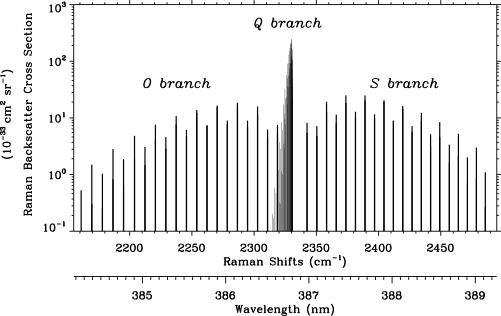
\includegraphics[width=\textwidth]{\currfiledir oe/OE_n2_fig1.pdf}
\caption{Raman-Spektrum von \ch{N2} in der Atmosphäre gemessen mit einem Laser der Wellenlänge 354.8~nm. Darstellung leicht modifiziert aus \cite{Liu14_OE_N2}. }
\end{figure}


\section{Wie misst man das?}

Moleküle ohne permanentes Dipolmoment (also beispielsweise homonukleare Moleküle) zeigen im THz-Absorptionsspektrum kein Rotationsspektrum. Moleküle ohne  Variation des Dipol-Moments mit der Normal-Koordinate zeigen kein Vibrationsspektrum im Infraroten. Solche
Moleküle sind trotzdem spektroskopierbar, nämlich über den Raman-Effekt.

Der Raman-Effekt\sidenote{nach Chandrasekhara Venkata Raman, 1888--1970} ist die \emph{inelastische} Streuung von Licht an Materie, bei der sich also die Frequenz des Lichts ändert. Dies ist im Gegensatz zur Rayleigh-Streuung, die die \emph{elastische} Streuung von Licht beschreibt. Nur wenige Photonen werden inelastisch gestreut. Der Effekt ist daher mit dem Auge nicht wahrzunehmen und man benötigt eine spektral schmale und intensive Lichtquelle, also einen Laser. Diesen scheint man auf bzw. durch die Probe.\sidenote{Wir diskutiere hier Raman-Spektroskopie an Gasen. Raman-Streuung an festen Proben wird aber ebenfalls sehr oft zur Charakterisierung von Materialien eingesetzt.} Im Gegensatz zu den Spektroskopie-Methoden, die wir bisher betrachtete haben, wird hier das Licht \emph{senkrecht zur Stahlrichtung} detektiert. So misst man nur gestreutes Licht, nicht direkt den Laser. In einem hochauflösenden Spektrometer findet man dann bei drei Frequenzbereichen Photonen
\begin{itemize} \setlength{\itemsep}{0pt}
\item bei der Laser-Frequenz $\bar{\nu}_\text{laser}$. Dies ist die elastische Rayleigh-Streuung.
\item bei $\bar{\nu} < \bar{\nu}_\text{laser}$ inelastisch unter Energieverlust  gestreutes Licht. Dies nennt man Stokes-Linie. Sie ist etwa $10^{5}$ mal schwächer als die Rayleigh-Linie.
\item bei $\bar{\nu} > \bar{\nu}_\text{laser}$ inelastisch unter Energiegewinn gestreutes Licht. Dies nennt man Anti-Stokes-Linie. Sie ist noch einmal $10$ bis $100$ mal schwächer als die Stokes-Linie.
\end{itemize}
Die hier als Stokes- bzw. Anti-Stokes-Linie bezeichneten 'Linien' besitzen eine deutliche Struktur, sehr analog zu den Rotations-Vibrations-Spektren und beinhalten die gleiche Information über das Molekül.


\section{Klassische Erklärung des Schwingungs-Raman-Effekts}

Wir beginnen mit einer klassischen, makroskopischen Erklärung des Raman-Effekts. Das Molekül habe kein permanentes Dipolmoment, sei aber polarisierbar mit der Polarisierbarkeit $\alpha$. Zunächst vernachlässigen wir auch Rotation und Vibration des Moleküls. Dann ist das induzierte Dipolmoment
\begin{equation}
p_\text{ind}(t) = \alpha E(t) = \alpha E_0 \cos \omega_0 t
\end{equation}
Das Dipolmoment oszilliert also mit der Lichtfrequenz $\omega_0$. Laut den Maxwell-Gleichungen strahlen bewegte Ladungen elektromagnetische Felder ab, so auch dieses oszillierende Dipolmoment. Dies ist die Rayleigh-Streuung. Genauere Rechnungen zeigen, dass die Intensität proportional zu $\omega^4$ ist. Der Himmel ist also blau, weil blaues Licht besser Rayleigh-Streuung macht.

Nun erlauben wir die Vibration des Moleküls. Die Polarisierbarkeit hängt dann, bei passenden Molekülen, vom Kern--Kern--Abstand $R$ ab. Dies nähern wie in einer Taylor-Reihe
\begin{equation}
\alpha = \alpha(R) = \alpha(R_0) + \left. \frac{\partial \alpha}{\partial R} \right|_{R_0}  \left( R - R_0 \right) + \dots
\end{equation}
Der Kern--Kern--Abstand $R$ ändert sich periodisch mit der Schwingungs-Frequenz $\omega_\text{vib}$ und der Amplitude $q$, also
\begin{equation}
\left( R - R_0 \right) = q \, \cos \omega_\text{vib} t
\end{equation}
Nun berechnen wir analog zu oben das induzierte Dipolmoment
\begin{align}
p_\text{ind}(t) = & \alpha(t) E(t) \\
= & \alpha(R_0) E_0 \cos(\omega_0 t) +
\left. \frac{\partial \alpha}{\partial R} \right|_{R_0}   q \,  E_0 \, \cos (\omega_\text{vib} t)  \cos(\omega_0 t) \\
= & \underbrace{  \alpha(R_0) E_0 \cos(\omega_0 t) }_\text{Rayleigh} \\
& + \left. \frac{\partial \alpha}{\partial R} \right|_{R_0}  \frac{ q \,  E_0 }{2} 
\Bigl\{ 
\underbrace{ \cos \left( [\omega_0 -\omega_\text{vib}] t \right)}_\text{Stokes}  +  \underbrace{\cos \left( [\omega_0 + \omega_\text{vib}] t \right)  
}_\text{Anti-Stokes} 
\Bigr\} 
\nonumber
\end{align}
Das durch das oszillierende Dipolmoment abgestrahlte elektromagnetische Feld liefert wieder die Rayleigh-, jetzt aber auch die Stoks- und Anti-Stokes-Linie.

Allgemein gilt, auch nach 'moderner' Rechnung, dass Schwingungsmoden dann Raman-aktiv sind, wenn die  Polarisierbarkeit von $R$ abhängt, also 
\begin{equation}
\left. \frac{\partial \alpha}{\partial R} \right|_{R_0} \neq 0
\end{equation}
Dies ist in zweiatomigen Molekülen \emph{immer} der Fall. In mehr-atomigen Molekülen \emph{mit Inversionssymmetrie} sind Raman-Aktivität und IR-Aktivität komplementär. Ein Beispiel dazu ist \ch{CO2}. Die symmetrische Streckschwingung ist nicht Infrarot-aktiv, aber im Raman-Spektrum sichtbar. Die asymmetrische Streckschwingung verhält sich genau umgekehrt.


\section{Mikroskopische Überlegungen}

Beim Raman-Prozess wechselwirken zwei Photonen mit dem Molekül, das einfallende und das auslaufende. Die quantenmechanische Beschreibung benötigt deshalb eine Störungstheorie zweiter Ordnung. Dies geht hier zu weit, ist aber beispielsweise in Kapitel 17 von \cite{Haken_wolf_II} dargestellt. Hier betrachten wir nur qualitative Argumente, die zumindest das Amplitudenverhältnis zwischen Stokes und Anti-Stokes-Linie erklären können. Diese sind nach obigen klassischen Überlegungen ja noch gleich stark.

Atome und Moleküle haben in der Quantenmechanik diskrete Energieniveaus. Photonen passender Frequenz können dann absorbiert werden. In der schematischen Darstellung verbindet ein senkrechter Pfeil zwei Niveaus.

\begin{marginfigure}
\begin{tikzpicture}
\begin{scope}
\draw[line width=1pt] (0,0) -- (1,0);
\draw[line width=1pt] (0,2) -- (1,2);
\draw[->] (0.5,0) -- (0.5,2);
\end{scope}
\begin{scope}[xshift=2cm]
\draw[line width=1pt] (0,0) -- (1,0);
\draw[line width=1pt, dashed] (0,2) -- (1,2);
\draw[->] (0.5,0) -- (0.5,2);
\end{scope}
\end{tikzpicture}
%\caption{Rotations-Vibrations-Übergänge liefert die P, Q, R-Zweige im Spektrum.}
\end{marginfigure}
 

Was passiert mit Photonen unpassender Frequenz? Diese können nicht absorbiert werden, dies würde schließlich die Energieerhaltung verletzten, aber sie werden gestreut. In der schematischen Darstellung zeichnet man dazu einen virtuellen Zustand als strichlierte horizontale Linie an das Ende des 'Photon'-Pfeils. Virtuelle Zustände können nicht bevölkert werden. Es gibt sie ja nicht wirklich. Auf der anderen Seite gibt es die Energie--Zeit--Unschärfe
\begin{equation}
\Delta E \cdot \Delta t \ge \hbar
\end{equation}
Wenn die Zeitdauer $\Delta t $ nur klein genug ist, dann muss die Energie-Unschärfe $\Delta E $ sehr groß werden. Für sehr kurze Zeiten kann man sozusagen gar nicht wissen, ob das Photon die passende Energie hat. Das kann man quantenmechanisch korrekt mit der Dichtmatrix formulieren. Für uns reicht hier, dass auch 'unpassende' Photonen mit diskreten Niveaus in Atomen oder Molekülen wechselwirken können, wenn auch nur für sehr kurze Zeit, wenige Femtosekunden für sichtbares Licht.

\begin{marginfigure}
\inputtikz{\currfiledir lorentz_oszillator}
\caption{Der dispersive Anteil des Lorentz-Oszillators fällt langsamer ab als der absorptive. }
\end{marginfigure}
 

Ein zweiter Gesichtspunkt kommt vom Lorentz-Oszillator aus Kapitel \ref{chap:3_diel}. Wir können diskrete atomare Übergänge als Lorentz-Oszillator beschreiben. Die Absorptionslinie hat das eben die bekannte Lorentz-Form. Sie fällt sehr schnell ab, wenn $| \omega  - \omega_0 |$ groß wird. Der Oszillator hat aber auch einen dispersiven Anteil, der den Realteil des Brechungsindexes beschreibt. Dieser fällt viel langsamer ab als der absorptive. Fern von der Resonanz ist er also wichtiger. Wir können uns ein Atom / Molekül fern von der Resonanz als als kleines Volumen mit einen etwas von Vakuum verschiedene Brechungsindex vorstellen, das aber nicht absorbiert. Solch eine Brechungsindex-Variation führt aber zu Streuung von Licht.

\begin{marginfigure}%[-50mm]
\inputtikz{\currfiledir fig_raman_states}
\caption{Stokes- und Anti-Stokes-Streuung über einen virtuellen Zustand (strichliert). Die spektrale Position de Rayleigh-Linie entspricht der des einfallenden Lasers.}
\end{marginfigure}
 

Nach diesen Vorüberlegungen können wir das Zustandsdiagramm für den Raman-Effekt zeichnen, wenn das Molekül mehrere äquidistante Schwingungszustände hat, die mit der Quantenzahl $\nu$ durchnummeriert sind. Der Abstand der Schwingungszustände $\hbar \omega_\text{vib}$ ist klein gegen die Energie des Photons $\hbar \omega_0$. Das Photon wird an einem virtuellen Zustand gestreut. Das dabei entstehende zweite Photon wird abgestrahlt und durch den Pfeil nach unten symbolisiert. Dieser Pfeil kann entweder auf den Ausgangszustand $\nu = 0$ zurück gehen. Das ist Rayleigh-Streuung. Oder er endet auf einem höheren Zustand und liefert die Stokes-Linien bei niedrigerer Energie. Die Anti-Stokes-Linien erhält man, wenn man nicht von $\nu = 0$ ausgeht, sondern von einem höheren Zustand, und dann aber bis auf $\nu = 0$ zurück fällt. Damit ist die Energie des auslaufenden Photons größer als die des einfallenden.



Damit lassen sich verschiedene Aspekte des Raman-Effekts erklären: er ist sehr schwach, weil zwei Photonen quasi gleichzeitig ($\Delta t \approx 1$~fs) wechselwirken müssen. Die Intensität der Linien ist proportional zur Besetzung der Ausgangs-Schwingungszustände, also entsprechend einem Boltzmann-Faktor
\begin{equation}
\frac{I_\text{anti-Stokes}}{I_\text{Stokes}} = 
\frac{N_{\nu = 1}}{N_{\nu = 0}} =
 e^{- \frac{\hbar \omega_\text{vib}}{k_b T}}
\end{equation}
Bei Vibrationsfrequenzen von etwa $1000$~cm$^{-1}$ und $k_B T \approx 200 $~cm$^{-1}$ bei Raumtemperatur ist das Intensitätsverhältnis also $e^{-5} \approx 1 /150$. Man kann das Verhältnis der Linien also als lokales Thermometer benutzen.

Die quantenmechanischen Rechnungen ergeben die selben Auswahlregeln wie für die Infrarot-Schwingungsspektroskopie, also 
\begin{equation}
 \Delta \nu = \pm 1 \quad \text{falls harmonisch, sonst} \quad \pm 1, \pm 2, \dots  
\end{equation}



\section{Der Rotations-Raman-Effekt}

Ähnlich zu molekularen Schwingungen findet sich auch die Rotation der Moleküle im Raman-Spektrum. Wir beginnen wieder mit dem klassischen Modell. Elektromagnetisches Feld $E(t)$ und induziertes Dipolmoment $p_\text{ind}(t)$ sind wie oben
\begin{equation}
p_\text{ind}(t) = \alpha(t) E(t) = \alpha(t) E_0 \cos \omega_0 t \label{eq:raman_pind_rot}
\end{equation}
In die Zeitabhängigkeit der Polarisierbarkeit $\alpha(t)$ bauen wir jetzt die Rotation ein. Dazu nehmen wir an, dass die Polarisierbarkeit anisotrop ist, sich also für zwei senkrecht aufeinander stehende Richtungen unterscheidet: $\alpha_\parallel \neq \alpha_\perp$. Bei einem sich mit der Kreisfrequenz $\omega_R$ drehenden Molekül ist die Polarisierbarkeit also
\begin{equation}
\alpha(t) = \alpha_0 + \Delta \alpha \cos ( 2 \omega_R t) \quad \text{mit} \quad \Delta \alpha = \alpha_\parallel - \alpha_\perp
\end{equation}
Der Faktor $2$ kommt daher, dass das Molekül bereits nach $180^\circ$ wieder in sich übergeht. Dies setzen wir wieder in Gl. \ref{eq:raman_pind_rot} ein und multiplizieren aus. Wir bekommen analog zu oben
\begin{align}
p_\text{ind}(t) = & \underbrace{  \alpha_0 E_0 \cos(\omega_0 t) }_\text{Rayleigh} \\
& +   \frac{ \Delta \alpha \,  E_0 }{2} 
\Bigl\{ 
\underbrace{ \cos \left( [\omega_0 -2 \omega_R] t \right)}_\text{Stokes}  +  \underbrace{\cos \left( [\omega_0 + 2 \omega_R] t \right)  
}_\text{Anti-Stokes} 
\Bigr\} 
\nonumber
\end{align}
Die Linien sind also bei der doppelten Rotationsfrequenz ober- oder unterhalb der Rayleigh-Linie. Quantenmechanische Rechnungen ergeben als Auswahlregeln entweder
\begin{equation}
\Delta J = 0 \quad \text{und falls} \quad  \Delta \alpha \neq 0 \quad  \text{dann auch} \quad \Delta J = \pm 2
\end{equation}
Die Position der Linien in einem Rotations-Raman-Spektrum sind also
\begin{equation}
 \bar{\nu} =  \bar{\nu}_\text{laser} \pm B \left[ (J+2) (J+3) - J(J+1) \right] = 
 \bar{\nu}_\text{laser} \pm B \left[ 4J + 6 \right]
\end{equation}
wobei das $+$ die Anti-Stokes-Banden und das $-$ die Stokes-Banden liefert. Der Abstand der äquidistanten Linien ist damit nicht mehr $2B$ wie im Fall des THz-Absorptions-Spektrums, sondern $4B$. Da $B$ klein gegenüber $\bar{\nu}_\text{laser} $ ist, ist ein reines Rotations-Raman-Spektrum messtechnisch aufwändig. Eine sehr schwache Linie muss in kleinem spektralen Abstand zur starken Rayleigh-Linie detektiert werden. Dies erfordert einen hochauflösenden und stark unterdrückenden Monochromator, quasi immer durch die Hintereinanderschaltung von zwei oder drei Monochromatoren zu einem Doppel- bzw. Trippel-Monochromator realisiert.




\begin{marginfigure}
\inputtikz{\currfiledir rot_vib_raman}
\caption{Rotations-Vibrations-Spektrum in Raman-Streuung. Alle gezeichneten Linien und Übergänge sind Stokes-Übergänge. Die Rayleigh-Linie liegt rechts außerhalb des Bildes, das entsprechende Anti-Stokes-Spektrum noch höherenergetischer. \label{fig:raman_rotvib}}
\end{marginfigure}

 \section{Rotations-Vibrations-Raman-Effekt}

Analog zum Rotations-Vibrations-Spektrum in Absorption lässt sich die kombinierte Anregung eines Rotations- und Schwingungsniveaus auch im Raman-Effekt beobachten. Abbildung \ref{fig:raman_rotvib} skizziert die beteiligten Zustände für die Stokes-Bande, also die Linien die niederenergetisch von der Rayleigh-Linie liegen. Die Linienpositionen sind 

\begin{equation}
 \bar{\nu} =  \bar{\nu}_\text{laser} \pm \bar{\nu}_\text{vib} \pm B \left[ 4J + 6 \right]
\end{equation}
Das erste $\pm$ unterscheidet zwischen Stokes ($-$) und Anti-Stokes ($+$). Das zweite $\pm$ entsprechend dem Vorzeichen von $\Delta J$. Man beachte, dass die Sequenz von äquidistanten Rotations-Linien wieder mit dem Abstand $6B$ von der reinen Vibrationslinie  $\Delta J = 0$ beginnt. Ähnlich zum Absorptionsspektrum werden die Linien mit $\Delta J =-2$ als O-Zweig, die mit 
$\Delta J =+2$ als S-Zweig bezeichnet.



\begin{margintable}
\begin{tabular}{rccccc}
$\Delta J$ & -2 & -1 & 0 & 1 & 2 \\
Zweig & O & P & Q & R & S
\end{tabular}
\caption{Nomenklatur der Zweige bei Rotationsspektren. $\Delta J = \pm 1$ im Absorptionsspektrum, $\Delta J = \pm 2$ im Raman-Spektrum sichtbar.}
\end{margintable}

\section{Einfluss der Kernspins}

Man beobachtet, dass das Rotations-Raman-Spektrum von zweiatomigen Molekülen aus zwei identischen Atomen eine charakteristische Intensitätsmodulation der Linien zeigt. Die Abbildung am Anfang des Kapitels ist ein Beispiel. Die Ursache dafür ist der Kernspin.

\begin{margintable}

\begin{tabular}{cc}
Molekül & $J_\text{ungerade}$  : $J_\text{gerade}$  \\ \hline
\ch{^1H2} & 3:1 \\
\ch{^2H2} & 1:2 \\
\ch{^{14}N2} & 1:2 \\
\ch{^{16}O2} & 1:0 
\end{tabular}
\caption{Beispiele für beobachtete Amplitudenverhältnisse.}
\end{margintable}


Atomkerne sind entweder Fermionen, haben also einen halbzahligen Spin, oder sie sind Bosonen, haben also einen ganzzahligen Spin. Für Fermionen muss die Gesamt-Wellenfunktion anti-symmetrisch unter Vertauschung sein, für Bosonen symmetrisch. Die Frage ist also, wie sich die einzelnen Komponenten der Wellenfunktion ändern, wenn wir die beiden Atomkerne im Molekül vertauschen.
 
Die \emph{Kernwellenfunktion} kann entweder die symmetrische oder die anti-symmetrische Kombination der beiden (identischen) Kernspins sein.
Die \emph{Elektronenwellenfunktion} ist gegenüber der Vertauschung der Kerne, also effektiv der Inversion der Koordinaten, fast immer symmetrisch. Prominente Ausnahme ist \ch{O2}, das einen Triplett-Grundzustand $^3\Sigma_g^-$ hat, wie wir bei der Diskussion der Termsymbole in Kapitel 3 gesehen haben. Die \emph{Vibrations-Wellenfunktion} ist immer symmetrisch gegen Vertauschung der Kerne. Die \emph{Rotations-Wellenfunktion} in zweiatomigen Molekülen ist anti-symmetrisch für ungerade Quantenzahlen $J$, also $J = 1,3, 5, \dots$ und symmetrisch für gerade $J$.


Die Symmetrie der Gesamt-Wellenfunktion ist das Produkt der einzelnen Symmetrien. Für fermionische Kerne muss die Gesamt-Funktion anti-symmetrisch sein, für bosonische Kerne symmetrisch. Damit beeinflusst die Symmetrie der Kern-Wellenfunktion die 'Geradheit' der Rotationsquantenzahl $J$. Und die statistischen Gewichte der beiden Symmetrien der Kern-Wellenfunktion ist unterschiedlich. Für Kerne mit $I = 1/2$ gibt es eine anti-symmetrische Kombination (analog dem Singulett für Elektronen) und drei symmetrische Kombinationen (analog dem Triplett für Elektronen). Allgemein ist das Verhältnis der statischen Gewichte $g$
\begin{equation}
 \frac{g_\text{symmetrisch}}{g_\text{anti-symmetrisch}} = \frac{I + 1}{I}
\end{equation}
Für fermionische Kerne ($I$ halbzahlig) ist damit 
\begin{equation}
 \frac{g(J = \text{ungerade}) }{g(J = \text{gerade})} = \frac{I + 1}{I}
\end{equation}
und für bosonische Kerne ($I$ ganzzahlig) gerade anders herum
\begin{equation}
 \frac{g(J = \text{ungerade}) }{g(J = \text{gerade})} = \frac{I}{I +1}
\end{equation}
Und wenn die elektronische Wellenfunktion  doch anti-symmetrisch sein sollte (Sauerstoff!), dann eben gerade andersherum.

\paragraph{Beispiel \ch{^1H2}} Jeder Kern hat $I = 1/2$, ist also ein Fermion und die Gesamt-Wellenfunktion muss anti-symmetrisch unter Vertauschen der beiden Kerne sein. Die Vibrations-Wellenfunktion und der elektronische Grundzustand sind symmetrisch, fallen bei der Multiplikation der Gesamt-Wellenfunktion also nicht ins Gewicht. Die Kern-Wellenfunktion kann sein
\begin{itemize}
\item \emph{anti-symmetrisch}, also $M_I = 0$. Damit die Symmetrie insgesamt anti-symmetrisch bleibt, muss der Rotationsanteil symmetrisch sein, also $J = \text{gerade}$. Dies nennt man \emph{para-Wasserstoff} und hat das statische Gewicht 1.

\item \emph{symmetrisch}, also $M_I = 0, \pm 1$. Damit die Symmetrie insgesamt anti-symmetrisch wird, muss der Rotationsanteil anti-symmetrisch sein, also $J = \text{ungerade}$. Dies nennt man \emph{ortho-Wasserstoff} und hat das statische Gewicht 3.
\end{itemize}
%
Da die Auswahlregeln $\Delta J = 2$ bei Raman-Übergängen verlangen, sind Übergänge ohne Änderung des Spins in einem Sub-System möglich. Es gibt im Wasserstoff-Molekül \ch{^1H2} also zwei Sätze von Linien, gerade und ungerade $J$, wobei die ungeraden um den Faktor 3 intensiver sind.




\paragraph{Beispiel \ch{^{16}O2}} Jeder Kern hat $I = 0$, ist also ein Boson und die Gesamt-Wellenfunktion muss symmetrisch unter Vertauschen der beiden Kerne sein. Die Vibrations-Wellenfunktion ist symmetrisch. Der elektronische Grundzustand $^3\Sigma_g^-$ ist allerdings eine Ausnahme, ein Triplett und damit anti-symmetrisch. Bei verschwindendem Spin $I=0$  der einzelnen Kerne ist die Summe der Kernspins immer Null. Damit gibt es nur eine Kern-Wellenfunktion und die ist symmetrisch. Damit die Gesamt-Wellenfunktion symmetrisch bleibt, muss die Rotations-Wellenfunktion anti-symmetrisch sein, also $J = \text{ungerade}$. In Sauerstoff-Molekül  \ch{^{16}O2} fehlen also die Rotationslinien mit geradem $J$ vollständig. Wenn man den Kernspin nicht berücksichtigen würde, dann würde man eine doppelt so große Rotationskonstante $B$ annehmen.





\printbibliography[segment=\therefsegment,heading=subbibliography]

\include{7_elec/7_elec}

\part{Festkörperphysik I}
%
%\renewcommand{\lastmod}{April 29, 2020}

\chapter{Kristallgitter}





\section{Ziele}

\begin{itemize}

\item Sie können das Konzept von mathematischem Punktgitter und physikalischer Basis benutzen, um Strukturen wie die unten gezeigte zu beschreiben.

\item Sie können die konventionelle Einheitszelle der häufigsten Bravais-Gitter erkennen und zeichnen, sowie die Wigner-Seitz-Zelle konstruieren.

\item Sie können die verschiedenen Arten der Bindung in einem Festkörper erklären und dabei das Konzept der Madelung-Konstante verwenden.

\end{itemize}


\begin{figure}
\inputtikz{\currfiledir intro}
%  \caption{Absorptions- und Fluoreszenz-Spektrum des Farbstoffs BODIPY  (\href{https://www.thermofisher.com/de/de/home/life-science/cell-analysis/labeling-chemistry/fluorescence-spectraviewer.html?SID=srch-svtool&UID=10001moh}{thermofischer.com}).}
\end{figure}



\section{Überblick}

Die Festkörperphysik demonstriert Lösungen für das Problem, ein System aus sehr viele Teilchen einfach zu beschreiben. In der Atomphysik haben wir einen Kern und im Wesentlichen ein Elektron betrachtet. Weitere Elektronen sind hinzugekommen, deren Wechselwirkung wurde aber quasi vernachlässigt. In der Molekülphysik hatten wir mehrere Atome, oft zwei, manchmal etwa 10. Wieder haben wir das System oft auf die Bewegung einer reduzierten Masse vereinfacht. Im Hückel-verfahren hatten wir eine Methode gesehen, mit der man viele Atome in einem Molekül behandeln kann. In der Festkörperphysik müssen aber nicht ein paar 10 oder 100 Atome, sondern etwa $10^{23}$ Atome behandelt werden. Das Diagonalisieren einer Matrix dieser Kantenlänge ist sicherlich unpraktikabel.

Die Festkörperphysik führt zu diesem Zweck Konzepte zur Behandlung sehr großer Systeme ein. Aus meiner Sicht sind die wesentlichen Konzepte 
\begin{itemize} \setlength{\itemsep}{0pt}
\item das {Kristallgitter}
\item der {reziproke Raum} als Fourier-Transformierte des Kristallgitters
\item das Quasi-Teilchen als Anregung eines Vielteilchen-Systems, die sich wie ein Teilchen benimmt
\item die Dispersionsrelation als Energie-Impuls-Darstellung, die zur Bandstruktur führt
\end{itemize}
In den folgenden vier Kapiteln werden wir diese Konzepte anhand der Kerne in einem Festkörper einführen und deren Effekte diskutieren. Im nächsten Semester in der Festkörperphysik II werden dann Effekte der Elektronen in Festkörpern besprochen werden. Dies ist dann auch das 'modernste' Kapitel der kanonischen Experimentalphysik mit Effekten wie der Supraleitung und dem Quanten-Hall-Effekt.

Wir betrachten hier und im Wesentlichen auch im nächsten Semester nur kristalline, also periodische Festkörper. Man kann die Festkörperphysik als Untermenge der Physik der kondensierten Materie betrachten, in der dann auch amorphe, also nicht-kristalline Festkörper sowie Flüssigkeiten, Gläser und Polymere betrachtet werden. Dies ist dann Thema von Spezialveranstaltungen im Master-Studiengang. 

In diesem Kapitel werden wir die Idee eines Kristallgitters einführen und Methoden zu seiner Beschreibung besprechen. Das sind sozusagen die 'Vokabeln', die wir für die folgenden Kapitel benötigen.


\section{Bravais-Gitter}

Eine Kristallstruktur besteht aus einem mathematischen Punktgitter und einer Basis,  die die Physik in Form von einem oder mehreren Atomen beinhaltet. Man kann sich die Basis als Kachel vorstellen, die entsprechend dem Muster des Punktgitters angeordnet wird. Wie wir sehen werden ist dabei die Wahl der Basis nicht eindeutig. Zunächst betrachten wir nur das mathematische Punktgitter. Dies trägt den Namen von Auguste Bravais.

Ein dreidimensionales (mathematische) Gitter ist eine Anordnung von (mathematischen) Punkten im Raum, die translationsinvariant ist unter jeder Translation $\mathbf{T}$
\begin{equation}
 \mathbf{T} = n_1 \mathbf{a}_1 + n_2 \mathbf{a}_2 + n_3 \mathbf{a}_3  
\end{equation}
wobei die $n_i$ beliebige ganze Zahlen sind und die \emph{Basis-Vektoren} $\mathbf{a}_i$ nicht alle in einer Ebene liegen. Das 'Basis' in diesen Basis-Vektoren hat nichts mit der oben genannten Basis zu tun, die die Physik beinhaltet. Ein beliebiger Vektor aus der Menge der möglichen Translationen $\mathbf{T}$ wird als \emph{Gittervektor} bezeichnet. Die Länge der Basis-Vektoren   $\mathbf{a}_i$, also  $a_i$, wird \emph{Gitterkonstante} genannt.

\begin{marginfigure}
\inputtikz{\currfiledir einheitszelle}

\caption{Primitive(dinkelgrau) und nicht-primitive (hellgrau) Basis-Vektoren und Einheitszellen.}
\end{marginfigure}


Die Wahl der Basis-Vektoren   $\mathbf{a}_i$ ist  bei gegebenem Punktgitter nicht eindeutig. Zum einen sind Linearkombinationen von  Basis-Vektoren ebenfalls möglich, zum anderen verlangt unsere Definition von $\mathbf{T}$ nicht, dass \emph{jeder} Gitterpunkt durch die Translation $\mathbf{T}$  erreicht werden muss.  $\mathbf{a}'_i = 2 \mathbf{a}_i$ ist also ebenfalls möglich. Wir grenzen die Wahl etwas ein, indem wir das durch die Basis-Vektoren   $\mathbf{a}_i$  definierte Volumen betrachten. Dies ist die \emph{Elementarzelle} oder \emph{Einheitszelle}. Basis-Vektoren, die das kleinste Volumen aufspannen, nennt man \emph{primitiven Basis-Vektoren} bzw. deren Volumen die \emph{primitive Einheitszelle}. Diese Einheitszelle beinhaltet nur einen Gitterpunkt.\sidenote{Wenn man Punkte an Seiten, Ecken, Kanten der Einheitszelle anteilig rechnet.} Allerdings sind auch die primitiven Basis-Vektoren immer noch nicht eindeutig. Wir werden weiter unten in der Wigner-Seitz-Zelle eine eindeutig definierte primitive Einheitszelle kennenlernen.

Wenn also die $\mathbf{a}_i$ primitive  Basis-Vektoren sind, dann sind \emph{alle} Punkte des Gitters durch 
\begin{equation}
 \mathbf{R} = n_1 \mathbf{a}_1 + n_2 \mathbf{a}_2 + n_3 \mathbf{a}_3  
\end{equation}
mit ganzzahligen  $n_i$ beschrieben. Eine äquivalente Definition des Bravais-Gitters ist, dass Anordnung und Orientierung der Gitterpunkte von jedem Gitterpunkt aus gesehen gleich aussieht.


\section{Klassifizieren von Bravais-Gittern durch deren Symmetrie}

Wieviel verschiedene Punktgitter kann es im dreidimensionalen Raum geben? Ein Gitter gilt dann als 'verschieden', wenn es eine andere Symmetrie besitzt. Einfach alle Achsen skalieren ändert nichts Relevantes. Mögliche Symmetrie-Operationen sind die oben eingeführten Translationen $\mathbf{T}$. Eine andere Art von Symmetrie-Operationen lässt einen einzelnen Gitterpunkt unverändert. Die Menge dieser Operationen nennt man \emph{Punktgruppe} und ist Teil der Gruppentheorie.

\paragraph{Drehung} Was ist der kleinste Winkel $\phi$, um den man ein Gitter drehen kann, so dass es wieder in sich über geht? Dieser Winkel wird in der Form $\phi = 2 \pi / n$ als Zähligkeit $n$ notiert\sidenote{Dies ist die Notation nach Hermann-Mauguin. Alternativ gibt es auch die nach Schoenflies, hier $C_1$, $C_2$ etc.}. Es können nur Werte $n= 1$, 2, 3, 4 und 6 auftreten. Auch im Zweidimensionalen gibt es keine Kacheln mit 5, 7 oder 8 Ecken.

\paragraph{Spiegelung} Bei der Spiegelung an einer Ebene wird nicht nur ein Punkt sondern eine ganze Ebene, in der er liegt, festgehalten. Diese Symmetrie wird durch ein $m$ gekennzeichnet, wenn die Drehachse in dieser Spiegel-Ebene liegt, und durch $/m$, wenn die Drehachse senkrecht auf der Spiegel-Ebene steht.

\paragraph{Inversion} Die Punktspiegelung wird durch $\bar{1}$ gekennzeichnet.

\paragraph{Drehinversion} Dies ist eine hilfreiche zusammengesetzte Symmetrie-Operation aus einer Drehung und anschließender Inversion, die durch die Zähligkeit mit Überstrich, also beispielsweise $\bar{3}$ dargestellt wird. 

Auf Basis der Dreh-Symmetrie\footcite{Hunklinger2014} können die mathematischen Punkt-Gitter in sieben Klassen unterteilt werden, die sogenannten Kristallsysteme. Im kubischen System gibt es also 4 Rotationsachsen mit jeweils dreizähliger Symmetrie, die vier Raumdiagonalen des Würfels. Die anderen Symmetrie-Operationen werden eine Rolle spielen, wenn wir eine Basis an das mathematische Gitter binden.



\begin{table}
\begin{tabular}{llll}
Kristallsystem 	& 	Symmetrie & Gitterkonstante & Winkel \\
triklin 	&  	$1$						& $a_1 \neq a_2 \neq a_3$ &  $\alpha \neq \beta \neq \gamma$\\
monoklin 	& 	 $2$ 					& $a_1 \neq a_2 \neq a_3$ &  $\alpha = \gamma = 90^\circ, \beta \neq 90^\circ$\\
orthorhombisch 	& 	  $22$  & $a_1 \neq a_2 \neq a_3$ &  $\alpha= \beta =  \gamma = 90^\circ$\\
%
tetragonal 	&  $4$ & $a_1 = a_2 \neq a_3$ &   $\alpha= \beta =  \gamma = 90^\circ$\\
 hexagonal 	& 	 $6$ & $a_1 = a_2 \neq a_3$ &  $\alpha = \beta = 90^\circ, \gamma = 120^\circ$\\
trigonal 	& 	  $3$  & $a_1 = a_2 = a_3$ &  $\alpha = \beta = \gamma \neq 90^\circ$\\
kubisch 	&  	$3333$  & $a_1= a_2=  a_3$ &  $\alpha= \beta =  \gamma = 90^\circ$\\
\end{tabular}
\caption{Die sieben Kristallsysteme. 
 Der Winkel $\alpha$ wird von $\mathbf{a}_2$ und  $\mathbf{a}_3$  eingeschlossen, etc.}
\end{table}


Man kann die sieben Kristallsysteme weiter unterteilen\footcite{Bergmann-Schaefer-FK,AshcroftMermin2013} durch Hinzunehmen der Translationssymmetrie $\mathbf{T}$. Effektiv bedeutet dies, dass wo möglich weitere Gitterpunkte hinzugefügt werden, wobei aber die  Rotationssymmtrie der Kristallsysteme erhalten bleibt. 
Dies führt auf die 14 Bravais-Gitter, die in Abbildung \ref{fig:gitter_bravais14} gezeigt sind. Es ist die Leistung von Auguste Bravais zu erkennen, dass es genau diese und keine weiteren mathematisch Punktgitter gibt. Gitter ohne zusätzliche Punkte werden primitiv genannt, die mit hinzugefügten Punkten basis-, flächen- oder raum-zentriert. Diese Punkte sind natürlich ebenfalls Gitterpunkte, völlig äquivalent zu den an den Ecken gezeichneten Punkten. Alle Punkte sind gleich. Man könnte für die Zeichnung einen anderen Satz Punkte aus der unendlichen Menge der Gitterpunkte herausgreifen, und dann könnten diese Punkte an den Ecken der Darstellung liegen. Damit sind die gezeigten Strukturen, die \emph{konventionellen Einheitszellen}, nur im Fall der primitiven Gitter auch primitive Einheitszellen, ansonsten gewöhnliche  Einheitszellen.



\begin{figure}
%\includegraphics[height=\textheight]{\currfiledir kristall/bravais.pdf}
\inputtikz{\currfiledir bravais_ML}



\caption{Die 14 Bravais-Gitter. \label{fig:gitter_bravais14}  Gezeigt sind die konventionellen Einheitszellen, die die Symmetrie  des Gitters möglichst gut wiedergeben, aber im Falle der zentrierten Gitter nicht primitiv sind.
}
\end{figure}


\section{Die Basis}


Während das Gitter ein mathematisches Konstrukt ist, eine symmetrische Anordnung von mathematischen Punkten im dreidimensionalen Raum, kommt durch die \emph{Basis} die Natur ins Spiel. Die Basis beschreibt die Position der Atome relativ zum Gitterpunkt. Es kann dabei ein oder mehrere Atome in einer Basis sein. Die Position des Atoms $j$ relativ zum zugehörigen Gitterpunkt ist dann 
\begin{equation}
 \mathbf{r}_j = x_{1,j} \mathbf{a}_1 + x_{2,j} \mathbf{a}_2 + x_{3,j} \mathbf{3}_1  
\end{equation}
mit $0 \le x_{i,j} \le 1$. Die Lage der Atome in der Basis relativ zu 'ihrem' Gitterpunkt ist nicht eindeutig, da die Gitterpunkte ja mathematische Konstrukte und daher nicht messbar sind.


Die Symmetrie der Basis hat einen Einfluss auf die Symmetrie des Kristalls. Die sieben Kristallsysteme des mathematischen Gitters werden 32 kristallographische Punktgruppen, wenn also Translationssymmetrie unberücksichtigt bleibt. Diese unterscheiden sich dann in den anderen oben genannten Symmetrie-Operationen.
Wenn wieder die Translationssymmetrie mit berücksichtigen wird ergeben sich 230 kristallographische Raumgruppen.


\section{Beispiel: Honigwaben-Gitter}

Als Beispiel betrachten wir ein zweidimensionales Honigwaben-Gitter wie in nebenstehender Abbildung gezeigt. Dieses Gitter ist kein Bravais-Gitter, auch wenn es sehr symmetrisch aussieht. Zwei benachbarte Gitter-Punkte unterscheiden sich darin, wie das Gitter in ihrer Umgebung orientiert ist. Das  Honigwaben-Gitter ist ein dreizählig rotationssymmetrisches Gitter mit einer zwei-atomigen Basis. Mit dieser Wahl ist das Gitter translationsinvariant. Die Lage der Atome in der Basis relativ zu 'ihrem' Gitterpunkt ist nicht eindeutig. Die Skizze zeigt verschiedene Möglichkeiten.



\begin{marginfigure}
\inputtikz{\currfiledir honigwabe}

\caption{Honigwaben-Gitter}
\end{marginfigure}


\section{Die Wigner-Seitz-Zelle}

Die Wahl der primitiven Einheitszelle ist nicht eindeutig. Mit der Wigner-Seitz-Zelle gibt es eine Konstruktionsvorschrift, mit der man immer auf eine eindeutige primitive Einheitszelle kommt.



\begin{marginfigure}
\inputtikz{\currfiledir wsz-2d}

\caption{Konstruktion der Wigner-Seitz-Zelle in 2D.}
\end{marginfigure}

\begin{marginfigure}
\inputtikz{\currfiledir wsz-3d}

\caption{Die Wigner-Seitz-Zelle des raum-zentrierten kubischen Gitters.}
\end{marginfigure}

Man wähle einen Gitterpunkt und konstruiere Verbindungslinien zu allen benachbarten Punkten. Auf diese Linien errichte man Mittelsenkrechten (im zweidimensionalen) bzw. eine zur Linie senkrechte Ebene in der Mitte der Linie (im dreidimensionalen). Durch diese Mittelsenkrechten bzw. Mittelebenen wird eine Fläche bzw. ein Volumen eingeschlossen, das den Startpunkt beinhaltet. Dies ist die Wigner-Seitz-Zelle.

Diese Zelle ist primitiv, da sie nur einen Gitterpunkt beinhaltet. Sie hat außerdem die gleiche Symmetrie wie das Gitter selbst. Die Konstruktionsvorschrift ist unabhängig von der konkreten Wahl der Gittervektoren. Die Abbildungen zeigen als Beispiel die Konstruktion in einem schiefwinkligen zweidimensionalen Gitter sowie die Wigner-Seitz-Zelle des kubisch-raumzentrierten Gitters.


\section{Wichtige Kristallstrukturen}


\paragraph{\ch{NaCl}}
Kristallines \ch{NaCl} besteht aus einem flächen-zentrierten kubischen Gitter (engl: face-centered cubic, fcc). Schon weil es zwei verschiedene Atome sind muss es eine Basis mit mindestens zwei Atomen geben. Hier sind es genau zwei Atome,  beispielsweise mit \ch{Na+} im Ursprung und \ch{Cl-} im Zentrum der konventionellen Einheizstelle, also bei
\begin{equation}
 \mathbf{r}_{Cl} = \frac{1}{2} \left(\mathbf{a}_1 + \mathbf{a}_2 +  \mathbf{a}_3  \right)
\end{equation}
wenn die $\mathbf{a}_i$ so gewählt sind, dass sie die konventionelle Einheitszelle aufspannen, also kartesisch sind. Dies ist auch die Struktur von \ch{LiF}, \ch{MgO}, \ch{CaTe}.



\paragraph{\ch{CsCl}}
Dies ist ein primitives kubisches Gitter (engl. simple cubic, sc), ebenfalls mit einer zwei-atomigen Basis mit 
\begin{equation}
 \mathbf{r}_{Cl} = \frac{1}{2} \left(\mathbf{a}_1 + \mathbf{a}_2 +  \mathbf{a}_3  \right)
\end{equation}
Dies ist auch die Struktur von \ch{CsI}, \ch{TlBr}.

\paragraph{\ch{Fe}} Eisen bildet ein kubisch-raumzentriertes Gitter (engl. body-centered cubic, bcc) mit nur einem Atom in der Basis.

\paragraph{Diamant} Kohlenstoff-Atome in einem Diamant-Kristall bilden ein fcc-Gitter (face-centered cubic), aber ebenfalls mit einer zwei-atomigen Basis. Eine Basis kann also auch identische Atome beinhalten. Die Positionen sind der Ursprung sowie um ein Viertel der Raum-Diagonalen verschoben in der konventionellen Einheitszelle, als
\begin{align}
 \mathbf{r}_{C_1} = & 0 \\
 \mathbf{r}_{C_2} = & \frac{1}{4} \left(\mathbf{a}_1 + \mathbf{a}_2 +  \mathbf{a}_3  \right)
\end{align}
Die Atome sind untereinander in der tetraederförmigen Bindung der $sp^3$-Hybridisierung verbunden. Dies ist auch die Struktur von \ch{Si}, \ch{Ge}.

\paragraph{\ch{ZnS}} Zinkblende (\ch{ZnS}) hat die gleiche Struktur wie Diamant. Jede Atomsorte bildet für sich ein fcc-Gitter. Gegeneinander sind die Gitter um ein Viertel der Raum-Diagonalen verschoben. Dies ist auch die Struktur von \ch{CdTe}, \ch{GaAs}, \ch{InP}.


\section{Dichteste Kugelpackung}

Man kann die Atome in einem Kristallgitter durch harte Kugeln ersetzen und dabei den Kugeldurchmesser maximal wählen, also so, dass die Kugeln sich berühren. Welcher Volumenanteil des Kristalls wird nun durch Kugeln ausgefüllt? Die maximale Packungsdichte ist 
\begin{equation}
 \frac{\pi}{3 \sqrt{2}} \approx 74 \%
\end{equation}
Um diese Packungsdichte zu erreichen, liegen die Kugeln in der untersten Lage A in einem zweidimensionalen hexagonalen Gitter. Jede Kugel ist also von fünf Nachbarn umgeben. In der nächsten Lage B liegen die Kugeln in den Mulden, die sich zwischen den unteren Kugeln bilden.  Die Größe der Kugeln erzwingt, dass nur jeder zweite Mulde besetzt wird.
Dies ist wieder ein zweidimensionales hexagonales Gitter. Für die dritte Lage gibt es zwei Möglichkeiten: entweder man besetzt die Mulden, die den Positionen in Lage A entsprechen, oder man besetzt die Mulden, die weder von der Lage A noch von der Lage B eingenommen werden. Im ersten Fall spricht man von der ABAB-Stapelfolge, im zweiten von der ABCABC-Folge.

\begin{marginfigure}
\inputtikz{\currfiledir stacking}

\caption{ABC-Stapelfolge (oben) und ABA-Folge (unten).}
\end{marginfigure}


Welchen Bravais-Gittern entsprechen diese Folgen?  Die Folge ABCABC bildet ein flächen-zentriert kubisches Gitter (fcc).  Die Raumdiagonale der  Einheitszelle steht senkrecht auf den Ebenen A, B und C. Diese Packung wird daher auch 'cubic closed packing' (ccp) genannt. Die Folge ABAB nennt man  'hexagonal closed packing' (hcp), weil sie ein (dreidimensionales) hexagonales Bravais-Gitter mit einer zwei-atomigen Basis bildet (mit $c=a \sqrt{8/3}$, siehe Abb. \ref{fig:gitter_bravais14}). Eine Kugel ist dabei am Ursprung der konventionellen Einheitszelle, die zweite bei 
\begin{equation}
 \mathbf{r}_{S_2} =  \frac{2}{3}  \mathbf{a}_1 + \frac{1}{3}  \mathbf{a}_2 + \frac{1}{2}  \mathbf{a}_3  
\end{equation}
 wobei die $\mathbf{a}_i$ die konventionelle Einheitszelle aufspannen.

Die kubische dichteste Kugelpackung wird beispielsweise von \ch{Au} und \ch{Ag} realisiert, die hexagonal dichteste Kugelpackung von \ch{Cd} oder \ch{Mg}. Es finden sich auch komplexere Abfolgen der Positionen A, B und C. Metalle aus der Gruppe der seltenen Erden bilden beispielsweise ABACABAC.






\section{Bindungen in Festkörpern}



Wie bei den Molekülen  sind es auch in den Festkörpern die Elektronen der Atome, die die Bindung bewirken. Man kann die verschiedenen Bindungen also nach der Verteilung der Elektronen unterscheiden. Im Gegensatz zu Molekülen bilden sich Festkörper auch aus Atomen mit abgeschlossenen Schalen. Die schwache van-der-Waals-Kraft bildet beispielsweise Edelgaskristalle bei niedrigen Temperaturen. In Ionenkristallen wird ein Elektron transferiert und die Coulomb-Anziehung  bestimmt die Bindung. Die kovalente Bildung in Festkörpern ist analog zur der in Molekülen. Als Extremfall gibt es die metallische Bindung, bei der manche Elektronen über den ganzen Kristall gleichmäßig verteilt sind und  ein freies Elektronengas bilden. Ein Sonderfall ist die Wasserstoff-Brückenbindung, die aber in der Biologie eine große Rolle spielt. Im Folgenden werden wir die für uns neuen  Bindungen besprechen.

\begin{marginfigure}
%\inputtikz{\currfiledir stacking}

\caption{Skizze Bindungstypen}
\end{marginfigure}



\section{Van-der-Waals-Bindung}

Die Van-der-Waals-Bindung ist sehr schwach (meV pro Atom), aber immer vorhanden. Sie wird also nur dann sichtbare, wenn andere Bindungskräfte nicht zum Tragen kommen, beispielsweise in Kristallen von Edelgas-Atomen.

Die Verteilung der Elektronen um einen Atomkern ist kein starres Gebilde. Die Elektronendichte-Verteilung fluktuiert und in einem Augenblick kann es ein netto Dipolmoment $\mathbf{p}_1$ bei Atom $1$ geben. Dieses Dipolmoment ist verknüpft mit einem elektrischen Feld, dessen Amplitude $E_1 \propto p_1 / r^3$ ist.\sidenote{Die Richtungsabhängigkeit ignorieren wir hier.} Ein Atom $2$ in der Entfernung $r$ wird dann durch dieses Feld polarisiert und es bildet sich ein induziertes Dipolmoment $p_2 = \alpha E_1 \propto 1/r^3$. Das Wechselwirkungspotential $\phi(r)$ ist damit das Potential von $\mathbf{p}_2$ im Feld $\mathbf{E}_1$, 
\begin{equation}
 \phi(r) = - \mathbf{p}_2 \, \mathbf{E}_1 \propto - \frac{B}{r^6}
\end{equation}
wobei die Konstante $B$ positiv und für das jeweilige Element charakteristisch ist.

Bei kleine Atom--Atom--Abständen kommt die abstoßende Kraft aufgrund des Pauli-Verbots hinzu. Oft modelliert man sie als $A/r^{12}$. Insgesamt ergibt sich damit das \emph{Lenard-Jones-Potential}
\begin{equation}
\phi(r) = \frac{A}{r^{12}} - \frac{B}{r^{6}} = 4 \epsilon \left[ \frac{\sigma}{r^{12}} -  \frac{\sigma}{r^{6}} \right]
\end{equation}
wobei $\epsilon$ die Tiefe und $\sigma$ den Nulldurchgang des Potentials, sozusagen den Radius des Atomrumpfes, bestimmt. Der Gleichgewichtsabstand ist $r_0 = 2^{1/6} \sigma \approx 1.12 \sigma$.

In einem Kristall wirkt dieses Potential zwischen allen Paaren von Atomen, also ist die Bindungsenergie 
\begin{equation}
U_B = \frac{1}{2} \sum_{m,n}^N \phi_{n,m} = 
2 N \epsilon \sum_{m=1,   \neq n}^N 
\left[ 
\frac{\sigma}{r_{nm}^{12}} -  \frac{\sigma}{r_{nm}^{6}} 
\right]
\end{equation}
Der Faktor $1/2$ kommt daher, dass man in der ersten Summe alle Bindungs-Paare doppelt zählt. Die zweite Summe läuft nur noch über einen Summanden, da der Kristall translationsinvariant ist und es daher ausreicht, von einem Atom ausgehend alle Bindungen zu betrachten.

Dies lässt sich weiter vereinfachen, in dem man den Atom--Atom--Abstand $r_{nm}$ schreibt als $r_{nm} = \rho_{nm} \, a$  mit der Gitterkonstanten $a$ im kubischen flächenzentrierten (fcc) Gitter:
\begin{align}
U_B = & 
2 N \epsilon 
\left[ 
\frac{\sigma^{12}}{a^{12}}
\sum_{m=1,   \neq n}^N  \frac{1}{\rho_{nm}^{12}} 
-
\frac{\sigma^{6}}{a^{6}}
\sum_{m=1,   \neq n}^N  \frac{1}{\rho_{nm}^{6}} 
\right] \\
\approx & 
2 N \epsilon 
\left[ 
12.13 \; \frac{\sigma^{12}}{a^{12}}
-
14.45 \; \frac{\sigma^{6}}{a^{6}}
\right] 
\end{align}
Das Minimum der Bindungsenergie im Kristall findet sich nun bei $r_0 \approx 1.09 \sigma$, also etwas näher als im vd-Waals-'Molekül'. Dieser Wert wird auch experimentell für die schwereren Edelgasatome gefunden.

\section{Ionische Bindung}

Bei der Ionischen Bindung dominiert die Coulomb-Anziehung zwischen unterschiedlich geladenen Ionen. Die van-der-Waals-Wechselwirkung vernachlässigen wir also. Am Beispiel von \ch{NaCl} diskutieren wir die einzelnen Beiträge zur Bindungsenergie.

Zunächst müssen wir beide Atome ionisieren
\begin{align}
 \ch{Na} + 5.14\text{ eV} \rightarrow  & \ch{Na+} + \ch{e-} \\
  \ch{e-}  + \ch{Cl} \rightarrow  & \ch{Cl-} + 3.16\text{ eV}
\end{align}
Wir müssen also netto 1.53 eV aufwenden, um ein Ionenpaar herzustellen.

Dann bringen wir die beiden Ionen aus dem Unendlichen zusammen, bis zum experimentell gefundenen Bindungsabstand von $R_0 = 2.81$~\AA. Die Coulomb-Energie bei diesem Abstand beträgt -5.1~eV. Insgesamt gewinnen wir also durch Bildung eines \ch{NaCl}-'Moleküls' 3.57~eV. Dabei ist aber der abstoßende Teil des Bindungspotentials und die Wechselwirkung mit allen anderen Ionen des Kristalls noch nicht berücksichtigt.

Analog zur van-der-Waals-Wechselwirkung setzen wir also wieder als Potential zwischen einem Paar von Ionen an
\begin{equation}
 \phi(r_{nm}) = \pm \frac{e^2}{4 \pi \epsilon_0 \, r_{nm}} + \frac{B}{ r_{nm}^{12}}
\end{equation}
Das wechselnde Vorzeichen berücksichtigt die abwechselnd anziehende und abstoßende Wechselwirkung, je nach Ladung des Ions. Wir bilden wieder die Summe über alle Paare
\begin{equation}
U_B = N \sum_{m \neq n} \, \phi(r_{nm})  = N \sum_{m \neq n} \, \phi(\rho_{nm} \, a) 
\end{equation}
wobei $N$ nun die Anzahl der Ionen einer Sorte bezeichnet und so der Faktor 2 überflüssig wird. Wir haben wieder die Abstände durch die Gitterkonstante ausgedrückt. Nun machen wir die Annahme, dass die Abstoßende Wechselwirkung kurzreichweitig ist und nur $z$ Ionen im Abstand $a$ beitragen. Damit wird  
\begin{align}
U_B = & + z \frac{ B}{ a^{12}} - N \sum_{m \neq n} \, \pm \frac{e^2}{4 \pi \epsilon_0 \, \rho_{nm} \, a}  \\
= & + z \frac{ B}{ a^{12}} - N \frac{e^2}{4 \pi \epsilon_0 \,  \, a}  \, \alpha
\end{align}
mit der \emph{Madelung-Konstante} $\alpha$
\begin{equation}
 \alpha = \sum_{m \neq n} \, \frac{\pm}{\rho_{nm} }  
\end{equation}
Die Madelung-Konstante hängt nur von der Art des Gitters ab. Ihre Berechnung erfordert allerdings ein paar Tricks, da die Reihe insbesondere im Dreidimensionalen nicht gut konvergiert. 

\begin{marginfigure}

\begin{tabular}{ll}
kubisch flächen-z. & $\alpha \approx 1.747$ \\
kubisch raum-z. & $\alpha \approx 1.763$ \\
Diamant & $\alpha \approx 1.64$ \\
\end{tabular}
\caption{Die Madelung-Konstante $\alpha$ hängt nur schwach vom Gitter-Typ ab.}
\end{marginfigure}

Am Gleichgewichts-Abstand ist die Ableitung nach der Gitterkonstante Null, wodurch sich $B$ bestimmen lässt. Damit ergibt sich für die Bindungsenergie pro Ion einer Sorte
\begin{equation}
\frac{U_B}{N} = \frac{e^2 \, \alpha }{4 \pi \epsilon_0 \, R_0} \, \left( 1- \frac{1}{12} \right) = U_\text{Coulomb} \, \alpha \, \left( 1- \frac{1}{12} \right) 
\end{equation}
Für \ch{NaCl} ergibt sich so ein Wert von -8.25~eV, nah am experimentell gefundenen Wert von -8.15~eV.





\section{Wasserstoffbrückenbindung}

In einer Wasserstoffbrückenbindung bildet ein Wasserstoff-Atom nicht eine kovalente Bindung zu einem anderen Atom, sondern zu zwei Atomen. Dies ist natürlich keine gewöhnliche kovalente Bindung. Dazu fehlt dem Wasserstoff  Bindungselektron.

Die Wasserstoffbrückenbindung entsteht, wenn das H-Atom stark kovalent an einen Bindungspartner gebunden ist. Bei geht das Elektron des H-Atoms fast vollständig auf den Partner über und es verbleibt quasi ein Proton. Dies wirkt anziehend auf andere negativ geladene Bindungspartner. Aus räumlichen Gründen\sidenote{Das Proton ist viel kleiner als alle Atome mit Elektronen} kann jeweils nur ein weiterer Bindungspartner wechselwirken. Die Bindung ist daher auch oft asymmetrisch, also \ch{A}$-$\ch{H}$--$\ch{B}. Typische Bindungsenergien sind 0.2~eV, bei \ch{HF} kann aber auch 1.6~eV erreicht werden.

Diese Bindung spielt in der Biologie eine große Rolle. Proteine sind typischerweise durch viele Wasserstoffbrückenbindung verbunden. Jede einzelne Bindung ist schwach, nicht viel stärker als $k_B T$, und kann so einfach geöffnet werden, um eine Funktionalität zu erzeugen. Gleichzeitig sind alle Bindungen zusammen stark, ähnlich einem Klettverschluss.





%-------------------




\printbibliography[segment=\therefsegment,heading=subbibliography]

\include{9_rezi/9_rezi}
%\renewcommand{\lastmod}{April 29, 2020}

\chapter{Phononen}





\section{Ziele}

\begin{itemize}
\item Sie können die  Dispersionsrelation $\omega = f(\mathbf{k})$ von Phononen (Abb. \ref{fig:phonon_intro}) benutzen, um die kollektive Bewegung der Atome zu beschreiben, und diese mit einfachen Modellen vergleichen.

\item Sie können die Teilchen-Eigenschaft von Phononen in Streuexperimenten erklären.

\end{itemize}




\begin{marginfigure}
\inputtikz{\currfiledir fig_gaas_intro}
\caption{Phononen-Dispersion in Gallium-Arsenid (\ch{GaAs}) (Daten aus \cite{Strauch_gaas}). \label{fig:phonon_intro}}

\end{marginfigure}


\section{Wie misst man das?}

Wir betrachten in diesem Kapitel eine kollektive Anregung aller Atome eines Kristalls in ihrer Schwingung um die Gleichgewichtsposition, die wir in den letzten beiden Kapitel betrachtet hatten. Dies entspricht den Normalmoden, die wir in der Molekülphysik bei der Schwingung der Moleküle betrachtet hatten. Nur versuchen wir hier nicht, eine Matrix zu diagonalisieren, sondern machen (raten) gleich einen passenden Ansatz. Wir werden sehen, dass die Anregung dieser Normalmoden nicht nur in ihrer Energie quantisiert ist ($E= (n + \frac{1}{2}) \hbar \omega$ überrascht wahrscheinlich nicht). Vielmehr benimmt diese Anregung der  Normalmoden sich wie ein punktförmiges Teilchen, das einen Impuls besitzt und mit dem man bei einem Stoß Energie und Impuls austauscht. Dieses Teilchen nennt man \emph{Phonon}.

Um Phononen zu vermessen, muss man also andere Teilchen an ihnen stoßen und Energie- und Impulsübertrag messen. Wegen des Welle-Teilchen-Dualismus kann man das auch als inelastische Streuung einer Welle am schwingenden Kristall beschreiben. Das ist die gleiche Streutheorie wie im letzten Kapitel, nur erlauben wir jetzt schwingende Atome und dadurch einen Energieübertrag.

\begin{marginfigure}
%\inputtikz{\currfiledir fig_gaas_intro}
\caption{3-Achs-Spektrometer}

\end{marginfigure}

Im Experiment macht man das beispielsweise durch inelastische Neutronenstreuung. Ein Neutronenstrahl wird in einem Kernreaktor oder in einer Spallationsquelle  hergestellt. Wichtig ist dabei, dass die Neutronen 'thermisch' sind, die kinetische Energie pro  Neutron also in etwa $k_B T$, also einige 10 meV beträgt. Diesen Neutronenstrahl leitet man in ein 3-Achs-Spektrometer. Dabei wird drei mal die Bragg-Beugung benutzt und jedes Mal der Winkel $\Theta$ des Strahls zu einem Kristall eingestellt. Die erste Bragg-Beugung wird benutzt, um eine Energie / Wellenlänge des Neutronenstrahls durch ihren Beugungswinkel zu selektieren. Am zweiten Kristall findet dann die inelastische Streuung statt. Hier werden die Phononen untersucht, und Ausbreitungsrichtung und Energie der Neutronen ändert sich. Die Richtung wird durch eine Reihe von Abschirmungen geometrisch festgelegt. Die Energieänderung wird gemessen, in dem an einem dritten Kristall wieder Bragg-Beugung zur Energiebestimmung benutzt wird. Schließlich muss man nur die die ankommenden Neutronen zählen. Man trägt das Ergebnis wie in Abb.~\ref{fig:phonon_intro} auf, als Energieänderung des Neutronen (=Frequenz der Phononen) über die Richtungsänderung der Neutronen (= Wellenvektor der Phononen).

\section{Einfaches Modell: lineare Kette}

Wir stellen die Schwingung der einzelnen Atome in einem Kristall als Superposition von ebenen Wellen dar. Die Atome bilden Ebenen, und alle Atome einer Ebene werden in gleichere Weise (Richtung und Amplitude) aus ihrer Ruhelage ausgelenkt. Die Schwingung findet also um eine Gleichgewichtsposition herum statt, die durch das in den letzten beiden Kapiteln beschriebene Gitter definiert ist. Wir nehmen ebenfalls an, dass die Schwingung harmonisch ist, was bei kleinen Auslenkungen sicherlich der Fall ist. Die Wahl der Kristall-Ebene bestimmt die Richtung des Wellenvektors $\mathbf{k}$ der ebenen Welle. Die Wellenlänge $\lambda$ den Betrag des Vektors $|\mathbf{k}| = 2 \pi / \lambda$. Weil alle Atome in der Ebene das gleiche tun, ist es möglich, allein eine lineare Kette von Atomen zu betrachten, zu der aus jeder Ebene nur jeweils ein Atom beiträgt.

Wir beschränken uns hier zunächst auf eine Auslenkung allein entlang der Richtung der Kette. Wir indizieren im Folgenden die Atome entlang der Kette mit den Indizes $s$ und $p$. Die Auslenkung eines Atoms an der Position $s$ aus der Gleichgewichtsposition sei $u_s$. 
Das zeitliche Mittel über $u_s(t)$ ist damit Null. Die Atome seien durch Federn verbunden. Die Kraft auf das Atoms $s$ ist dann
\begin{equation}
F_s = \sum_p \, c_p \left( u_{s+p} - u_s \right)
\end{equation}
mit der Federkonstante $c_p$, die beschreibt, die das betrachtete Atom mit dem $p$ Gitterpositionen weiter verknüpft ist. Es geht also nur die relative Auslenkung der Atome zueinander ein. Die Bewegungsgleichung wird damit
\begin{equation}
M \frac{d^2 \, u_s}{dt^2} = \sum_p \, c_p \left( u_{s+p} - u_s \right)
\end{equation}
wobei wir angenommen haben, dass alle Atome die gleiche Masse $M$ besitzen. Mit dem Ansatz einer ebenen Welle\sidenote{entsprechend den Nornmalmoden in der Molekülphysik} wird die Auslenkung des Atoms mit den Index $s+p$ zu
\begin{equation}
u_{s+p} = U_0 \, e^{-i ( \omega t - \mathbf{k} \cdot \mathbf{a} (s+p) )}
\end{equation}
mit dem Wellenvektor $\mathbf{k}$ im reziproken Raum und dem Gittervektor $\mathbf{a}$ im Realraum. Der Term $\mathbf{a} (s+p)$ beschreibt also die  Gleichgewichtsposition des betrachteten Atoms im Realraum, also das, was wir in den letzten beiden Kapiteln diskutiert hatten. Wenn wir diesen Ansatz in die Bewegungsgleichung einsetzen erhalten wir
\begin{equation}
- \omega^2 \, M = \sum_p \, c_p \left( e^{i \mathbf{k} \cdot \mathbf{a} p} - 1 \right)
\end{equation}
Da ja alle Atome identisch sind, gilt $c_p = c_{-p}$ und damit
\begin{equation}
 \omega^2 =  \frac{2}{M} \, \sum_{p=1}^\infty \, c_p \left( 1 - \cos ( \mathbf{k} \cdot \mathbf{a} p ) \right)
\end{equation}
Den hier gefundenen Zusammenhang zwischen Eigenfrequenz $\omega$ der Oszillation und Länge (und Richtung) des Wellenvektors $\mathbf{k}$ nennt man \emph{Dispersionsrelation}.





\section{Allein nächste Nachbarn wechselwirken}

Nun machen wir zusätzlich die Annahme, dass nur nächste Nachbarn miteinander wechselwirken, dass es also nur Federn zwischen direkt benachbarten Atomen gibt. Damit sind nur dir $c_{\pm 1}$ von Null verschieden und die Summe fällt weg. Wir ziehen jetzt auch die Wurzel und erhalten
\begin{equation}
\omega = \sqrt{\frac{4 \, c_1}{M}} \left| \sin (\frac{1}{2} \, \mathbf{k} \cdot \mathbf{a}  ) \right|
\end{equation}

\begin{marginfigure}

\inputtikz{\currfiledir kette_1atom}
\caption{Dispersionsrelation der einatomigen Kette}
\end{marginfigure}


\paragraph{Grenzfall langer Wellenlänge} Falls die Wellenlänge der ebenen Welle gegen unendlich geht, dann geht $k = 2 \pi \ \lambda$  gegen Null. Damit wird das Argument des Sinus sehr klein gegen Eins und wir können die Kleinwinkelnäherung anwenden:
\begin{equation}
\omega = \sqrt{\frac{4 \, c_1}{M}} \frac{1}{2}  |\mathbf{k}| | \mathbf{a}| \propto k
\end{equation}
Die Dispersionsrelation ist in der Nähe von $k = 0$ also linear in $k$. Die Schallgeschwindigkeit $v$ ist frequenzunabhängig
\begin{equation}
 v = \frac{\omega}{k} = a  \sqrt{\frac{ c_1}{M}}  = \text{const.}
\end{equation}



\paragraph{Physikalisch bedeutsamer Bereich von $\mathbf{k}$} 

\begin{marginfigure}
\inputtikz{\currfiledir outside_BZ}

\caption{Eine Welle mit dem Wellenvektor $k + G = k + 2\pi /a$ beschreibt die gleiche Auslenkung der Atome wie die mit dem Wellenvektor $k$.  Vektoren innerhalb der ersten Brillouinzone sind ausreichend, um alle möglichen Bewegungsmuster zu beschreiben. \label{fig:phonon_k_plus_g} }
\end{marginfigure}


Wir betrachten das Verhältnis der Auslenkung benachbarter Atome, also
\begin{equation}
 \frac{u_{s+1}}{u_s}  = 
 \frac{U_0 e^{i \mathbf{k} \cdot \mathbf{a} (s+1) } } 
        {U_0 e^{i \mathbf{k} \cdot \mathbf{a} s}} 
         = e^{i \mathbf{k} \cdot \mathbf{a}}
\end{equation}
Dieser Ausdruck ist periodisch in $\mathbf{k}$. Alle möglichen Werte werden bereits abgedeckt im Intervall $- \pi < \mathbf{k} \cdot \mathbf{a}  < \pi$, bzw. in einer Dimension 
 \begin{equation}
 - \frac{\pi}{a} < k <  \frac{\pi}{a}
 \end{equation} 
Dies ist gerade die erste Brillouin-Zone. Werte von $k$ außerhalb dieser Zone beinhalten keine weitere Information. Sie beschreiben die gleiche Auslenkung der Atome. Die Funktion  $e^{i \mathbf{k} \cdot \mathbf{a}}$ wird nur an den Gitterpositionen ausgewertet. Welchen Wert sie an anderer Stelle annimmt spielt keine Rolle. Für $k$ außerhalb der ersten Brillouin-Zone oszilliert die Funktion zwischen den Gitterpositionen schneller, was aber keine physikalische Konsequenz hat.



\paragraph{Gruppengeschwindigkeit}
Die Gruppengeschwindigkeit beschreibt die Geschwindigkeit eines Wellenpakets und damit die Ausbreitung von Information
\begin{equation}
v_g = \frac{d \omega}{d k} =
 \sqrt{\frac{c_1 \, a^2}{M} } \, \cos 
 \left( \frac{1}{2} \mathbf{k} \cdot \mathbf{a} \right)
\end{equation}
An den Grenzen der Brillouin-Zone, bei $k = \pm \pi / a$ wird damit die Gruppengeschwindigkeit Null. Dies entspricht einer stehenden Welle.






\section{Lineare zweiatomige Kette}

Nun heben wir die Annahme auf, dass alle Atome identisch sind. Wir betrachten eine Kette, die abwechselnd aus zwei Atomsorten besteht. In der Sprache eines Gitters ist hat diese also eine zweiatomige Basis. Die Gitterkonstante $a$ ist der (kürzest) Abstand zwischen \emph{identischen} Atomen. Hier nehmen wir an, dass sich die Atome in ihrer Masse unterscheiden. Die Federn seien aber wieder nur zwischen nächsten Nachbarn (also verschiedenen Atomsorten) und sie seine alle identisch\sidenote{Man könnte auch identische Massen und alternierende Federn annehmen.} Der Index $s$ bezeichnet nun die Einheitszelle (nicht das Atom). Wir unterscheiden zwischen den Atomen, in dem die eine Sorte um $u_s$, die andere um $v_s$ ausgelenkt sein soll.  Die Reihenfolge entlang der Kette ist also $u_{s-1}$ ---  $v_{s-1}$ --- $u_{s}$ ---  $v_{s}$ --- $u_{s+1}$ ---  $v_{s+1}$. Damit werden die Bewegungsgleichungen
\begin{align}
 M_1 \frac{d^2 u_s}{dt^2} = & c \, \left( v_s + v_{s-1} - 2 u_s \right) \\
 M_2 \frac{d^2 v_s}{dt^2} = & c \, \left( u_s + u_{s-1} - 2 v_s \right) 
\end{align}
wobei $c$ hier die einzige Federkonstante bezeichnet ($c_1$ von oben) und die $M_{1,2}$ die Masse der beiden Atomsorten ist.
Wir machen den Ansatz
\begin{align}
  u_s   = & u \,   e^{i \mathbf{k} \cdot \mathbf{a}  s} \, e^{-i \omega t} \\
  v_s  = & v  \, e^{i \mathbf{k} \cdot \mathbf{a}  s} \, e^{-i \omega t}
\end{align}
und erhalten zwei Lösungen für die Eigenfrequenz $\omega$ und damit die Dispersionsrelation
%\begin{equation}
%\omega^2 = c \, \frac{M_1 + M_2}{M_1 M_2}
%\pm \frac{c}{M_1 M_2} \sqrt{ (M_1 + M_2)^2 - 4 M_1 M_2 \sin^2 \left( \frac{1}{2}  \mathbf{k} \cdot \mathbf{a} \right) } 
%\end{equation}
%oder
\begin{equation}
\omega^2 =  \frac{c}{\mu}
\pm c \sqrt{ \frac{1}{\mu^2} - \frac{4}{M_1 M_2}  \sin^2 \left( \frac{1}{2}  \mathbf{k} \cdot \mathbf{a} \right) } 
\end{equation}
mit der reduzierten Masse $\mu = (M_1  M_2)/(M_1 + M_2)$. Die Dispersionsrelation besteht also aus zwei Zweigen, je nach Vorzeichen des $\pm$: Das negative Vorzeichen beschreibt den \emph{akustischen Zweig}. Er geht exakt in die einatomige Kette über, wenn man $M_1 = M_2$ setzt und $a$ entsprechend anpasst. Auch für $M_1 \neq M_2$ ist der akustische Zweig sehr ähnlich der einatomigen Kette, insbesondere linear zu $k$ in der Nähe von $k=0$. Das positive Vorzeichen beschreibt den \emph{optischen Zweig}. Für $k \rightarrow 0$ geht hier die Frequenz $\omega$ nicht gegen Null sondern gegen $\sqrt{2 c / \mu}$. Am Rand der Brillouin-Zone, also bei $k = \pi /a $ wird der Sinus Eins und damit\sidenote{Man zieht den Term $M_1 - M_2$ aus der Wurzel und macht dabei die Annahme $M_1 > M_2$.}
\begin{align}
\omega_+ = & \frac{2 c}{M_2} \\
\omega_- = & \frac{2 c}{M_1} 
\end{align}
Die Aufspaltung der Äste am Rand der Brillouin-Zone geht also mit dem Verhältnis der Massen $M_1 / M_2$. Diese Aufspaltung führt zu einer \emph{Bandlücke}: Im Frequenzbereich zwischen $\omega_- $ und $\omega_+$ gibt es keine Lösung der Bewegungsgleichung, unabhängig vom Wellenvektor $\mathbf{k}$. In einer solchen Kette von mit Federn verbundenen Massen können sich keine Wellen ausbreiten, deren Frequenz wischen $\omega_- $ und $\omega_+$ liegt. Wenn eine Masse von außen mit einer solchen Frequenz getrieben würde, dann bliebe diese Bewegung auf die nähere Umgebung beschränkt und weit entfernte Massen würden in Ruhe bleiben.




\begin{marginfigure}

\inputtikz{\currfiledir kette_2atom}
\caption{Dispersionsrelation der zweiatomigen Kette}
\end{marginfigure}

Die Bezeichnung der beide Äste als akustisch und optisch ergibt sich aus dem Schwingungsmuster bei kleinem $k$. Man findet
\begin{align}
 u = &v &&  \text{akustischer Zweig} \\
  \frac{u}{v} = &- \frac{M_2}{M_1} &&  \text{optischer Zweig} 
\end{align}
Im akustischen Zweig folgen also beide Atomsorten einer gemeinsamen Schwingungsmuster, wie man es für eine Schallwelle erwartet. Im optischen Zweig bleibt der Schwerpunkt ruhen ($u M_1 = - v M_2$). Wenn die beiden Atomsorten allerdings unterschiedliche (Teil-)Ladungen besitzen, dann führt diese Schwingung zu einem oszillierenden Dipolmoment und ist somit optisch anregbar, also Infrarot-aktiv.


\begin{marginfigure}
\inputtikz{\currfiledir muster}
\caption{Schwingungsmuster bei langen Wellenlängen: \textit{oben}: akustische Mode, \textit{unten}: optische Mode. Dargestellt ist jeweils die Auslenkung als Funktion des Ortes.}
\end{marginfigure}





\section{Moden im Dreidimensionalen}

Im allgemeinen Fall sind im dreidimensionalen diverse Schwingungsmoden vorhanden. Man kann diese wie folgt klassifizieren.

\paragraph{Transversal oder longitudinal} Die Auslenkung der Atome aus der Gleichgewichtsposition kann in Richtung des Wellenvektors $\mathbf{k}$ erfolgen (longitudinale Schwingung), oder senkrecht dazu (transversale Schwingung). Dabei ist die transversale Schwingung zweifach entartet, weil es zwei Richtungen gibt, die senkrecht auf $\mathbf{k}$ stehen.


\paragraph{Akustisch  oder optisch} Auch bei $p > 2$  Atomen in der Basis kann man wie im letzten Abschnitt verfahren. Man findet eine akustisch Mode, in der $u = v = w = \dots$, und $p -1$ optische Moden, in denen manche Atome außer Phase schwingen.

Zusammen ergeben sich damit folgende Moden \\
\begin{tabular}{rl}
$1$ & longitudinal akustisch (LA)\\
$2$ & transversal akustisch (TA) \\
$p-1$ & longitudinal optisch (LO) \\
$2(p-1)$ & transversal optisch (TO) \\
\end{tabular} \\
also insgesamt $3p$ Mode, wie man bei $p$ Atomen pro Basis und 3 Dimensionen erwarten würde.






\section{Streuung am schwingenden Gitter}

Wir betrachten noch einmal die Streuung einer Welle an einer Anordnung von Streuzentren, wie im letzten Kapitel, nur erlauben wir jetzt, dass die Streuzentren sich leicht um ihre Ruheposition bewegen
\begin{equation}
\mathbf{r}_m(t) = \mathbf{R}_m + \mathbf{u}_m(t) \quad \text{mit} \quad \left<\mathbf{u}_m(t)\right> = 0
\end{equation}
Die Amplitude der auslaufenden ebenen Welle mit der Richtungsänderung $\mathbf{K} = \mathbf{k}_\text{out} - \mathbf{k}_\text{in}$ ist
\begin{equation}
A_S(t) \propto e^{-i \omega_0 t} \, \sum_m e^{-i \mathbf{K} \cdot \mathbf{r}_m(t)} =
e^{-i \omega_0 t} \, \sum_m e^{-i \mathbf{K} \cdot \mathbf{R}_m}  e^{-i \mathbf{K} \cdot \mathbf{u}_m(t)}
\end{equation}
Da die Amplitude der Schwingung $\mathbf{u}_m(t)$ klein ist gegenüber der Gitterkonstanten und gilt für den interessanten Bereich von $\mathbf{K}$ dass  $\mathbf{K} \cdot\mathbf{u}_m(t) \ll 1 $. Daher können wir die zweite Exponentialfunktion in einer Reihe entwickeln und nach dem ersten Glied abbrechen.\sidenote{Das zweite Glied braucht man unten für den Debye-Waller-Faktor.}
\begin{equation}
 e^{-i \mathbf{K} \cdot \mathbf{u}_m(t)} \approx 1 - i \mathbf{K} \cdot \mathbf{u}_m(t)
\end{equation}
Die Auslenkungen $\mathbf{u}_m(t)$ beschrieben wir wieder wie oben als ebene Wellen, wobei wir hier den Wellenvektor $\mathbf{q}$ nennen statt $\mathbf{k}$, um ihn vom Vektor der gestreuten Welle zu unterscheiden. Der Einfachheit halber betrachten wir auch nur akustische Moden. Damit wird
\begin{equation}
\mathbf{u}_m(t) = \sum_\mathbf{q} \mathbf{U}_\mathbf{q} \, 
e^{ \pm i ( \mathbf{q} \cdot \mathbf{R}_m - \omega_\mathbf{q} t ) }
\end{equation}
Alles zusammen erhalten wir damit
\begin{equation}
A_S(t) \propto 
\sum_m e^{-i \mathbf{K} \cdot \mathbf{R}_m}  
e^{-i \omega_0 t} 
-
\sum_m \sum_\mathbf{q}  i \mathbf{K} \cdot \mathbf{U}_\mathbf{q} \,
 e^{-i (\mathbf{K} \pm \mathbf{q} ) \cdot \mathbf{R}_m}  
e^{-i (\omega_0 \pm \omega_\mathbf{q})  t} 
\end{equation}
Der erste Term ist die schon aus dem letzten Kapitel bekannte elastische Streuung. Hier geht die Bewegung der Streuzentren nicht ein. der zweite Term ist die inelastische Streuung, die proportional zur Amplitude $\mathbf{U}_\mathbf{q}$ der Schwingung der Streuzentren ist. Für die elastische Streuung hatten wir im letzten Kapitel gesehen, dass die Summe über alle Atompositionen nur dann einen Beitrag liefert, wenn die Bedingung $\mathbf{K} = \mathbf{G}$ erfüllt ist. Für die inelastische Streuung liefert die gleiche Argumentation die Bedingung
\begin{equation}
 \mathbf{K} \pm \mathbf{q} = \mathbf{G} \quad \text{und} \quad \omega_\text{out} = \omega_0 \pm \omega_\mathbf{q}
\end{equation}
Die Energie / Frequenz der gestreuten Welle ändert sich also bei inelastischer Streuung, wie beim Raman-Effekt in der Molekülphysik.



%\section{Inelastische Streuung}
%
%Im letzten Kapitel zur Strukturbestimmung hatten wir die Streuung von Röntgen-Strahlen oder andere (Materie-)Wellen benutzt. Dies war \emph{elastische} Streuung. Die Wellenlänge bzw. der Betrag des Wellenvektors $\mathbf{k}$ hat sich dabei nicht verändert, nur seine Richtung. Um die Phononen-Dispersion zu messen benötigen wir \emph{inelastische} Streuung. Gleichzeitig mit der Änderung der Richtung des Wellenvektors soll sich auch sein Betrag ändern. Dabei wird Energie von der Welle an die Gitterschwingung abgegeben oder davon aufgenommen. 

Die Bedingung lässt sich durch Multiplikation mit $\hbar$ als 
 Energie- und Impulserhalten schreibt 
\begin{align}
\hbar \omega_{out} = & \hbar \omega_{0}  \pm \hbar
 \omega_\mathbf{q} \\
\hbar \mathbf{k}_{out} =  &\hbar \mathbf{k}_{0} \pm \hbar 
\mathbf{q}  + \hbar \mathbf{G}
\end{align}
Dies ist ein wichtiger Schritt! Bei der Streuung (und anderen Effekten) verhalten sich Gitterschwingungen so als wären sie ein Teilchen. Dieses Teilchen nennt man \emph{Phonon}. Es hat die Energie $\hbar \omega_\mathbf{q}$ und den Impuls $\hbar \mathbf{q}$. Das positive Vorzeichnen beschreibt die Absorption (Vernichtung) eines Phonons, das negative die Emission (Erzeugung). Der Impuls $\hbar \mathbf{G}$ wird auf den gesamten Kristall übertragen, ohne dabei Energie zu übertragen.\sidenote{Wie beim Abprallen eines Balles von einer Wand.} Der Impuls des Phonons ist allerdings kein 'echter' Impuls, sondern nur ein Quasiimpuls oder Kristallimpuls, da ihm der Massetransport im Sinne von $p = m v$ fehlt. Manchmal nennt man das Phonon ein 'Quasiteilchen', manchmal ist dieser Term aber auch für modifizierte ('dressed') elementare Teilchen reserviert.\sidenote{Siehe 'quasiparticle' in engl. wikipedia.} Zumindest beschreibt es eine kollektive Anregung und ist damit ein Boson, weil natürlich eine Gitterschwingung mehr oder weniger stark angeregt sein kann und somit viele identische Phononen existieren können.






\section{Experimente}

Man kann inelastische Streuung genauso wie elastische Streuung mit diversen Arten von (Materie-)Wellen betreiben. Diese unterscheiden sich aber in ihre Energie bei gegebener Wellenlänge. Da bei inelastische Streuung am Ende ein Energieunterschied von $\hbar
 \omega_\text{phonon} $ gemessen werden soll, fällt dies je nach Art der Welle mehr oder weniger schwierig aus.
 
 \begin{table}
 \begin{tabular}{lll}
          & Wellenlänge & Energie \\
   Laser & 5320 \AA & 2.3 eV \\
   Röntgen & 0.1 \AA & 100 keV \\
   Neutronen & 1 \AA & 100 meV \\
 \end{tabular}
 \caption{Typische Energien und Wellenlängen}
 \end{table}

Bei der Dispersionsrelation der Phononen ist der relevante Bereich des Wellenvektors $q$ durch die erste Brillouin-Zone, also $| q | \le \pi / a$ gegeben.  Die Änderung des Wellenvektors der (Materie-)Welle $\mathbf{K}$ ist vom Betrag her maximal $4 \pi / \lambda$ (von $+\mathbf{k}_0$ zu $-\mathbf{k}_0$). Daher muss die Wellenlänge $\lambda$ sinnvollerweise kleiner als $2a$ sein, also im Bereich von wenigen Angstrom liegen.
 Die Wellenlänge von sichtbarem Licht ist also viel zu lang, um die gesamte Brillouin-Zone abzudecken. Energieänderungen  von einigen meV sind im Sichtbaren aber noch gut zu messen. Bei Röntgenstrahlen wird dies sehr schwierig, so dass Neutronenstreuung die Methode der Wahl ist, da hier die Energie der Phononen eine deutliche Änderung der Energie der Neutronen bewirkt.




\section{Inelastische Neutronenstreuung}


Die Streubedingung konstruiert man auch im inelastischen Fall mit der Ewald-Kugel, wie im letzten Kapitel. Nur kommt hier nun zusätzlich der Vektor $\mathbf{q}$ des Phonons hinzu, der entweder zu $\mathbf{k}_0$ addiert oder subtrahiert wird. Je nach dem liegt $\mathbf{k}$ dann entweder innerhalb\sidenote{$|k|$ kleiner, $\lambda$ größer, $\omega$ kleiner als im einfallenden Strahl, also Emission eines Phonons} oder außerhalb der Kugel, aber nicht mehr auf der Ewald-Kugel wie im elastischen Fall.

Man misst also für jede Richtungsänderung $\mathbf{K}$ die Änderung der Energie / Frequenz des Neutronenstrahls. Zusammen mit der bekannten Struktur und Orientierung des Kristallgitters und damit der Gittervektoren $\mathbf{G}$ kann man so die vollständige Dispersionrelation der Phononen bestimmen.

\begin{marginfigure}
\inputtikz{\currfiledir ewald_inelastisch}
\caption{Ewald Kugel inelastisch}
\end{marginfigure}




\newpage

\section{Beispiel: Kupfer}




\begin{marginfigure}
\inputtikz{\currfiledir fcc-3d_2x}
\caption{Punkte hoher Symmetrie in der Brillouin-Zone werden durch große Buchstaben gekennzeichnet. der $\Gamma$-Punkt ist die Mitte der BZ, also $k=0$. Der Pfad $\Gamma$--X--K--$\Gamma$--L nutzt aus, das Punkte mehrfach  vorkommen. \label{fig:phonon_pfad} }
\end{marginfigure}


Kupfer bildet einen kubisch-flächenzentrierten Kristall mit einatomiger Basis. Der reziproke Raum ist also kubisch-raumzentriert. Die Gitterkonstante beträgt 3.6~\AA. Abb. \ref{fig:phonon_kupfer} zeigt die Dispersionsrelation der Phononen, die durch inelastische Neutronenstreuung gemessen wurde. Aufgetragen ist die Frequenz $\nu$ des Phonons (aus der Änderung der Energie der Neutronen) über dem Wellenvektor $\mathbf{q}$, der sich aus der Änderung des Wellenvektors des Neutronenstrahls ergibt. Der Wellenvektor $\mathbf{q}$ ist in Form seines Miller-Indexes angegeben, der ja gerade den Vorfaktoren vor den primitiven reziproken Gittervektoren $\mathbf{b}_i$ entspricht. Die horizontale Achse ist mit dem Wert $\zeta$ beschriftet, der ein- oder mehrmals im Miller-Index vorkommt. Alle
 dargestellten Wellenvektoren sind damit entweder parallel zu einem reziproken Gittervektor (erstes Intervall), parallel zur Flächendiagonalen (zweites Intervall) oder parallel zur Raumdiagonalen (drittes Intervall). Die horizontale Achse ist entsprechend dem Betrag des Wellenvektors 
 $|\mathbf{q}|$ skaliert, d.h. der Abstand $\zeta = 0 \dots 0.5$ verhält sich wie $1$ zu $\sqrt{2}$ zu $\sqrt{3}$. Die gesamte Abbildung stellt die Frequenz der Phononen entlang einem Pfad im reziproken Raum dar, der in Abbildung \ref{fig:phonon_pfad}  dargestellt ist. Dabei kann man ausnutzen, dass reziproke Gittervektoren $\mathbf{G}$ addiert werden können ohne etwas  zu verändern (siehe Abb. \ref{fig:phonon_k_plus_g})
 
	\begin{figure}
\inputtikz{\currfiledir fig_copper_all}
\caption{Phononen-Dispersion in Kupfer (Daten aus \cite{Svensson_cu}). \label{fig:phonon_kupfer}}
\end{figure}

Die Dispersionsrelation ähnelt zumindest in Richtungen hoher Symmetrie, also [001] und [111]	dem einfachen Modell der linearen einatomigen Kette. Es gibt nur akustische Zweige, weil nur ein Atom in der Basis vorhanden ist. Die transversalen Moden sind entlang der hoch-symmetrischen Richtungen zweifach entartet. In die Richtung [110] wird die Entartung aufgehoben.


\section{Beispiel: Galliumarsenid (\ch{GaAs})}


Galliumarsenid (\ch{GaAs}) besitzt ebenfalls eine kubisch-flächenzentrierte Kristallstruktur, aber mit einer zweiatomigen Basis, eben eine Zinkblende-Struktur. Die Gitterkonstante der konventionellen Einheitszelle beträgt 5.7~\AA. Die Abbildung zeigt analog zu oben die Dispersionrelation. Wir finden nun auch einen optischen Zweig, da zwei Atome in der Basis sind. Die transversalen Zweige sind wieder in die hoch-symmetrische [001] und [111] Richtung entartet. In die [110] Richtung ist diese Entartung aufgehoben und wir finden 6 Zweige (2 Atome mal 3 Raumrichtungen).


\begin{figure}
\inputtikz{\currfiledir fig_gaas_all}
\caption{Phononen-Dispersion in \ch{GaAs} (Daten aus \cite{Strauch_gaas} ).}
\end{figure}



\section{Inelastische Streuung von Licht: Raman und Brillouin}

Der Wellenvektor eines sichtbaren Photons ist viel kürzer als der Rand der Brillouin-Zone also
\begin{equation}
 k_\text{Licht} = \frac{2 \pi}{\lambda} \ll k_\text{phonon} \approx \frac{\pi}{a}
\end{equation}
Das Verhältnis ist etwa 1:1000. Wenn man die Dispersionsrelation von Phononen und Photonen ins gleiche Diagramm zeichnet, dann sind die Photonen ein quasi senkrechter Strich. Mit sichtbarem Licht kann man daher die Dispersionsrelation der Phononen nur in der Nähe von $k \approx 0$ messen. Wenn dabei optische Phononen erzeugt oder vernichtet wird, dann entspricht dies der Raman-Streuung aus der Molekülphysik und Energieunterscheiden von Stokes- und Anti-Stokes-Linie von einigen 10 meV. Wenn akustische Phononen involviert sind, dann bezeichnet man dies als Brillouin-Streuung mit Energieunterscheiden von etwa 0.1 meV, die nur sehr aufwändig messbar sind.


\section{Anwendung: Akusto-optischer Modulator}

Akustische Phononen finden in Form des  akusto-optischen Modulators eine wichtige Anwendung in der Optik: eine laufende longitudinale Ultraschallwelle, also akustische Phononen, entspricht einer periodische Modulation des Brechungsindex des Materials. Dies ist damit ein Phasengitter für einen Lichtstahl, der senkrecht zur Ultraschallwelle durch das Material läuft. Der Lichtstahl wird damit an dem Gitter gebeugt und in verschiedene Ordnungen aufgespalten.

Dies kann auf verschiedene Weisen genutzt werden. In einfachsten Fall als Schalter: nur wenn die Ultraschallwelle anliegt existiert eine erste Beugungsordnung. Damit kann ein Strahl schnell (ns) an- und aus-geschaltet werden, wenn man den Ultraschall-Generator schaltet. Durch Variation der Amplitude der Ultraschallwelle kann eine beliebige Amplituden-Modulation des Lichtstahls erreicht werden.

Die Beugung in die erste Ordnung entspricht der Absorption eines Ultraschall-Phonons, die in die minus erste Ordnung der Emission. Damit ist klar, dass die Beugung auch mit einer Frequenzverschiebung einher geht. Es muss schließlich Energie- und Impuls-Erhaltung gelten. Auf diese Weise ist es möglich, sehr schmalbandige und frequenzstabile Laser im sichtbaren Spektralbereich (Frequenz ca. 300 THz) um die Frequenz des Phonons (ca. 10--100 MHz) zu verstimmen. Wenn man die Frequenz des  Ultraschall-Generators kontinuierlich ändert, dann kann man so einen kleinen Frequenzbereich kontrolliert abfahren.

Gleichzeitig ändert sich damit auch der Beugungswinkel. So kann ein Lichtstrahl sehr schnell in verschiedene, kontinuierlich änderbare Richtungen abgelenkt werden, was in manchen optischen Mikroskopen Verwendung findet.




%-------------------




\printbibliography[segment=\therefsegment,heading=subbibliography]

%\renewcommand{\lastmod}{April 29, 2020}

\chapter{Wärmekapazität der Phononen}





\section{Ziele}

\begin{itemize}
\item Sie dewe

\item S.

\end{itemize}


%\begin{figure}
%\inputtikz{\currfiledir fig_bodipy}
%  \caption{Absorptions- und Fluoreszenz-Spektrum des Farbstoffs BODIPY  (\href{https://www.thermofisher.com/de/de/home/life-science/cell-analysis/labeling-chemistry/fluorescence-spectraviewer.html?SID=srch-svtool&UID=10001moh}{thermofischer.com}).}
%\end{figure}



\section{Wärmekapazität}


Die Wärmekapazität eines Stoffes beschreibt den Zusammenhang zwischen der Änderung der Temperatur $T$ durch die Änderung der inneren Energie $U$ beispielsweise durch Wärmezufuhr, also
\begin{equation}
 C_V = \left( \frac{\partial U}{\partial T} \right)_{V = \text{const.}}
\end{equation}
bei konstantem Volumen $V$ des Stoffes. Messtechnisch ist $C_P$, also die Wärmekapazität bei konstantem Druck $P$ einfacher, jedoch ist die theoretische Beschreibung von $ C_V $ einfacher. Bei Festkörpern ist der Unterschied gering, da diese sich (zumindest im Vergleich zu Gasen) wenig mit steigender Temperatur ausdehnen.

Im Experiment findet man, dass die Wärmekapazität fester Stoffe mit der Temperatur steigt und sich dem Wert des Gesetze von Dulong-Petit annähert
\begin{equation}
 C_V = 3 \, N_A \, k_B \approx 25 \text{~J} \text{~mol}^{-1} \text{~K}^{-1}
\end{equation}
Der Verlauf von $ C_V$ bei niedrigeren Temperaturen ist eine einfach zu bestimmende makroskopische Größe, die viel über den mikroskopischen Aufbau des Festkörpers aussagt. Wir werden sehen, dass sie zumindest bei Nichtleitern vollständig durch die quantisierte  Gitterschwingungen und so die Teilcheneigenschaft der Phononen bestimmt ist. Das Modell dazu geht auf A. Einstein zurück, auch wenn er bei der Zustandsdichte $D(\omega)$ vereinfachende Annahmen getroffen hat. Die Innere Energie $U(T)$ ist
\begin{equation}
U(T) = \int_{\omega=0}^{\infty} \, \hbar \omega \, \braket{ n (\omega, T) } \, D(\omega) \, d\omega \label{eq:wk_u_allg}
\end{equation}
Bei jeder Frequenz $\omega$ existieren Phononen in der Dichte $D(\omega)$ der möglichen Zustände pro Frequenzintervall, der Energie pro Phonon $\hbar \omega$ und der Besetzung $\braket{ n (\omega, T) } $. Die Innere Energie ist dann das Integral über alle Frequenzen, und die Wärmekapazität die Ableitung davon nach der Temperatur $T$.


\section{Zustandsdichte im reziproken Raum $D(k) \, dk$ }

Zunächst betrachten wir nicht die eigentlich benötigte Zustandsdichte im Frequenzraum $D(\omega) d\omega$ sondern die im reziproken Raum $D(\k) dk$. Die Argumentation und die Rechenschritte sind dabei die selben, die auch bei der Herleitung der optischen Modendichte bei der Schwarzkörperstrahlung verwendet wurde\sidenote{z.B. Vorlesung EPB2 Atome, Kerne, Teilchen}, auf die wir weiter unten eingehen werden.

Bisher hatten wir uns über die Länge unsere ein- oder mehratomigen Kette keine Gedanken gemacht. Wenn sie endlich lang sein soll, was ja notgedrungen der Fall ist, dann können die Enden entweder frei sein, also keine Kraft auf sie wirken, also $\ddot{u} = 0$ sein. Oder sie können fest sein, also ohne Bewegung, also $u=0$. Eine dritte Möglichkeit sind periodische Randbedingungen, also eine ringförmige Kette mit $u_0 = U_N$ bei $N$ Atomen in der Kette. Wir benutzen hier diese Randbedingung, die anderen geben ähnliche Ergebnisse. Die Auslenkung der Masse am Index $s$ ist mit dem Ansatz der ebenen Welle
\begin{equation}
 u_s = u \, e^{- i \omega \, t} \, e^{i s \mathbf{k} \cdot \mathbf{a}}
\end{equation}
mit dem Wellenvektor $\mathbf{k} $ im reziproken Raum und dem Gittervektor $\mathbf{a}$ im  Realraum. Die Randbedingung $u_0 = U_N$ erfordert dann
\begin{equation}
 N \, k \, a = 2 \pi \, n
\end{equation}
wobei $n$ eine beliebige ganze Zahl ist und wie die Beträge der Vektoren eingesetzt haben.
Die Gesamtlänge der Kette ist $L = N a$ und damit kann $k$ nur diskrete Werte annehmen, die den Abstand $\Delta k$ haben
\begin{equation}
\Delta  k = \frac{2 \pi }{L} 
\end{equation}
Die Dichte $ D(k) \, dk$ der möglichen Werte von $k$ auf der $k$-Achse ein Wert pro $\Delta k$, also
\begin{equation}
 D(k) \, dk = \frac{L}{2 \pi} \, dk
\end{equation}
Die Zustandsdichte ist im $k$-Raum also konstant.
Analog kann man im Zwei- oder Dreidimensionalen verfahren, also bei Quadraten oder Kuben der Kantenlänge $L$. Die Zustandsdichte ist
\begin{equation}
D(k) = \frac{N_\text{EZ}}{V_{BZ}}  = 
\frac{V_\text{Kristall}} {(2 \pi)^d} =
 \left(\frac{L}{2 \pi} \right)^d 
\end{equation}
mit der Dimensionalität $d$ und der Anzahl der Einheitszellen $N_\text{EZ}$.

Was ist hier passiert? Die physikalisch sinnvollen Werte von $k$ waren schon im letzten Kapitel nach oben beschränkt, weil es nicht hilft, wenn die Welle schneller oszilliert als der Abstand der Atome ist. Bei einem Ring von Atomen ist nun aber auch nicht jede Wellenlänge wählbar, da nur stehende Wellen auf dem Ring möglich sind.\sidenote{Analog stehende Wellen auf einer endlichen Kette mit freien / festen Randbedingungen} Mögliche Werte der Wellenlänge haben die Form $\lambda_0 / n$, und damit mögliche Werte des Wellenvektors $n / \lambda_0$. Dadurch wird die $k$-Achse diskret. Dies spielt aber nur bei der Zustandsdichte eine Rolle, da die Punkte so dicht liegen, dass dies höchstens bei sehr kleinen Kristallen auflösbar ist.

Aus dem Blickwinkel der Normalmoden findet sich das gleiche Ergebnis. Bei $p$ Atomen je Einheitszelle und $N_\text{EZ}$ Einheitszellen im Kristall erwarten wir $3 p \, N_\text{EZ}$ Normalmoden. In der Dispersionsrelation der Phononen gibt es dann $3p$ Äste und $N_\text{EZ}$ diskrete Werte auf der $k$-Achse, also ebensoviele Zustände für Phononen wie Normalmoden.




\section{Zustandsdichte im Frequenz-Raum $D(\omega) \, d\omega$ }

Eine Zustandsdichte ist die Anzahl von Zuständen in einem festen Intervall, bisher einem festen Intervall auf der $k$-Achse, jetzt auf der $\omega$-Achse. Da der Zusammenhang zwischen Wellenvektor und Frequenz kein konstanter Faktor ist, ist dies nicht völlig trivial. Die Wahl des Intervalls ist typischerweise in der Variablen der Zustandsdichte kodiert, also $D(x)$ meint eigentlich $D(x) \, dx$. Es ist trotzdem sinnvoll, das $dx$ möglichst oft explizit mit zu schreiben.

Im Eindimensionalen können wir einfach mit $d \omega$ erweitern
\begin{equation}
D(k) \, dk  =  \frac{L}{2 \pi}\, \frac{dk}{d\omega} \, d\omega 
= \frac{L}{2 \pi}\, \frac{1}{v_g} \, d\omega
= D(\omega) \, d\omega
\end{equation}
mit der Gruppengeschwindigkeit $v_g = d\omega / dk$.

Im Zwei- oder Dreidimensionalen gehen wir einen anderen Weg. Wir nutzen aus, das im reziproken Raum die Zustände äquidistant sind, die Zustandsdichte also konstant ist. Alle Zustände bei gegebenem, festem $\omega$ bilden die Fläche\sidenote{in 3D, sonst Kurve in 2D} $S(\omega)$. Die Zustände bei $\omega + d\omega$ bilden eine weitere Fläche. Wir zählen somit die Zustände im Intervall $d\omega$, indem wir das Volumen zwischen den beiden Flächen bestimmen in mit der Zustandsdichte im $k$-Raum multiplizieren
\begin{equation}
D(\omega) d\omega = \left( \frac{L}{2 \pi} \right)^d \, \int_{\omega = \text{const.}}^{\omega + d\omega = \text{const.}} \, d \mathbf{k}
\end{equation}
Das Volumenelement $d \mathbf{k}$ teilen wir auf in einen Teil entlang der Fläche konstanter Frequenz $S(\omega)$ und einem Teil senkrecht dazu:  $d \mathbf{k} = dk_\perp \, dS_\omega$. Damit kann man dann die Gruppengeschwindigkeit schreiben als
\begin{equation}
v_g = \left| \frac{d\omega}{d \mathbf{k}} \right| 
=\left| \frac{d\omega}{d k_\perp} \right|
\end{equation}
und so
\begin{equation}
d \mathbf{k} = dk_\perp \, dS_\omega = dS_\omega \frac{d \omega}{|v_g|}
\end{equation}
Damit erhalten wir
\begin{equation}
D(\omega) d\omega = \left( \frac{L}{2 \pi} \right)^d \, d\omega \, \int_{\omega = \text{const.}}\,   \frac{1}{|v_g|} \, dS_\omega
\end{equation}
Wir müssen also nur noch ein Oberflächenintegral über eine Fläche Konstanter Frequenz $\omega$ ausführen und dabei den Kehrwert der Gruppengeschwindigkeit integrieren. Einfach wird dies im isotropen Fall, wenn die Frequenz $\omega$ der Phononen nur vom Betrag des Wellenvektors $k$ abhängt und nicht von seiner Richtung. Damit sind die Flächen konstanter Frequenz Kugeln mit dem Radius $k$. Und Die Gruppengeschwindigkeit ist dann natürlich auch konstant über die Kugeloberfläche. Wir erhalten dann
\begin{equation}
D(\omega) d\omega = \left( \frac{L}{2 \pi} \right)^3 \,     \frac{ 4 \pi \, k^2 }{|v_g|}   \, d\omega \label{eq:WK_dos_omega}
\end{equation} 
wobei $k$ hier als $k(\omega)$ zu verstehen ist.

Sowohl im eindimensionalen als auch im dreidimensionalen Fall geht die Gruppengeschwindigkeit als Kehrwert ein. In der zweiatomigen Kette beispielsweise geht diese asymptotisch gegen Null in der Nähe der Bandlücke, wodurch der Integrand in Gl.~\ref{eq:WK_dos_omega} divergiert. Diese Punkte nennt man \emph{van Hove Singularitäten}. Im Eindimensionalen divergiert hier die Zustandsdichte. In zwei und drei Dimensionen finden sich davon noch endlich hohe Spitzen und $D(\omega) \propto \sqrt{\omega_\text{van Hove} - \omega}$.


\section{Beispiele}

\begin{marginfigure}
\caption{1D zweiatomige Kette und Zustandsdichte}
\end{marginfigure}


Kupfer und SIlizium


\section{Einstein-Modell der Wärmekapazität}

Gehen wir zurück zur inneren Energie als Summe über die Energien der Phononen in Gl.~\ref{eq:wk_u_allg}. Wir hatten dazu (wie auch im Kapitel davor) die Phonnen als die Quanten der Gitterschwingung angenommen. Jedes Phonon trägt die Energie $\hbar \omega$ bei. Phononen sind Bosonen, d.h. jede Gitterschwingung ist mehrfach anregbar, was die unterschiedliche Auslenkung beschreibt. Damit wird die Besetzungsfunktion $\braket{n (\omega,T) }$ eine Bose-Einstein-Verteilung
\begin{equation}
\braket{n (\omega,T) } = \frac{1}{e^{\frac{\hbar \omega}{k_B \, T} }- 1}
\end{equation}



Einstein macht nun auch die weitergehende Annahme, dass nur ein Oszillator zur  Zustandsdichte beiträgt, also $D(\omega) \propto \delta(\omega_0 - \omega)$. Damit wird Gl.~\ref{eq:wk_u_allg}.
\begin{equation}
U(T) =  3N \, \frac{\hbar \omega_0 }{e^{\frac{\hbar \omega_0}{k_B \, T} }- 1}
\end{equation}
bei $N$ Atomen im Kristall. Die Wärmekapazität ist die Ableitung davon nach der Temperatur $T$
\begin{equation}
C_V = \frac{\partial U}{\partial T }  =3 N \, k_B \, 
\left( \frac{\hbar \omega_0}{k_B \, T} \right)^2 
\, \frac{e^{\frac{\hbar \omega_0}{k_B \, T} }}
{\left( e^{\frac{\hbar \omega_0}{k_B \, T} }- 1 \right)^2}
\end{equation}
Bei großen und kleinen Temperaturen $T$ geht dies gegen
\begin{align}
\text{für } k_B \, T \gg \hbar \omega_0  \quad & C_V \approx 3 N \, k_B \\
\text{für } k_B \, T \ll \hbar \omega_0  \quad & C_V \approx e^{-\frac{\hbar \omega_0}{k_B \, T} }
\end{align}
Damit haben wir glücklicherweise das Dulong-Petit-Gesetz bei hohen Temperaturen wiedergefunden. Bei niedrigen Temperaturen steigt die Wärmekapazität exponentiell mit der Temperatur.

Experimentell findet man auch diesen exponentiellen Anstieg, insbesondere wenn die wirkliche Zustandsdichte $D(\omega)$ im relevanten Energie- / Temperatur-Bereich durch einen starken Peak dominiert wird. Ein gutes Beispiel ist Diamant. Insbesondere bei noch tieferen Temperaturen findet man dann aber auch eine Abweichung vom Einstein-Modell, wenn eben die breite Verteilung der Zustände beiträgt und die Zustände im Peak selbst nicht mehr populiert sind.



\section{Debye-Modell der Wärmekapazität}

Die Näherung der Zustandsdichte als deltaförmig ist schon weitgehend. Im Modell von P. Debye wird ein größerer Frequenzbereich erlaubt. Es macht die Annahme, dass die Phasengeschwindigkeit $v$ für alle Wellenvektoren $k$ konstant ist. Im letzten Kapitel hatten wir gesehen, dass dies für die akustischen Phononen in der Nähe von $k \approx 0$ gilt. Hier wird nun angenommen, dass es bis zu $k = \pi / a$ gilt, und dass nur akustische Phononen vorhanden sind, also nur ein Atom in der Basis.

Die Dispersionsrelation ist also $\omega = v \, | \mathbf{k} |$ und somit die Zustandsdichte
\begin{equation}
D(\omega) d\omega = \left( \frac{L}{2 \pi} \right)^3 \,     \frac{ 4 \pi \, \omega^2 }{v^3}   \, d\omega 
\end{equation} 
quadratisch in der Frequenz $\omega$. Die maximale Frequenz, bis zu der die Zustandsdichte quadratisch steigt, wird Debye-Frequenz $\omega_D$ genant und ergibt sich aus dem Gesamtzahl der Zustände, also der Zahl $N$ der Atome im Kristall
\begin{equation}
N = \int_0^{\omega_{D}}  \left( \frac{L}{2 \pi} \right)^3 \,     \frac{ 4 \pi \, \omega^2 }{v^3}   \, d\omega 
\end{equation}
Man erhält mit $N = (L / a)^3$
\begin{equation}
\omega_{D} = v \, \frac{\pi}{a} \, \sqrt[3]{6 / \pi}
\end{equation}
Der Term $\sqrt[3]{6 / \pi}$ verdient etwas Aufmerksamkeit. Wir haben in diesem Modell Zustände angenommen, die alle innerhalb einer Kugel im reziproken Raum mit Radius $k_{D} = \omega_{D} / v$ liegen. In manche Richtungen ragt diese Kugel über den Rand der ersten Brillouin-Zone hinaus, der bei $k = \pi / a$ liegt. In den  Ecken der kubischen Brillouin-Zone hat der Wellenvektor  aber den Betrag $k = \pi / a \sqrt{3}$. Diese Ecken liegen außerhalb der Kugel, da $\sqrt{3} \approx 1.73 > 1.24 \approx \sqrt[3]{6 / \pi}$.


Die inneren Energie  (Gl.~\ref{eq:wk_u_allg}) wird im Debye-Modell
\begin{equation}
U = \int_0^{\omega_D} \, \hbar \omega \,  \left( \frac{L}{2 \pi} \right)^3 \,     \frac{ 4 \pi \, \omega^2 }{v^3}  \,
\frac{1}{e^{\frac{\hbar \omega}{k_B \, T} }- 1} \, d\omega
\end{equation}
Wir führen die Debye-Temperatur $\Theta$ ein mit $k_B \, \Theta = \hbar \omega_D$ und die Abkürzungen
\begin{equation}
x = \frac{\hbar \omega}{k_B T} \quad \text{und} \quad
x_D = \frac{\hbar \omega_D}{k_B T}  = \frac{\Theta}{T}
\end{equation}
und erhalten für die Wärmekapazität
\begin{equation}
C_V = 9 N \, k_B \, \left(\frac{T}{\Theta} \right)^3 \,
\int_0^{x_D} \frac{x^4 \, e^x}{\left(  e^x - 1 \right)^2} \, dx
\end{equation}
Für hohe Temperaturen, also $x_D \rightarrow 0$, also $\hbar  \omega_D \ll k_B \, T$ finden wir wie erwartet das Dulong-Petit-Gesetzt. Für tiefe Temperaturen also $x_D \rightarrow \infty$, also $\hbar  \omega_D \gg k_B \, T$  erhalten wir
\begin{equation}
C_V = \frac{12 \pi^4}{5} \, N \, k_B \, \left(\frac{T}{\Theta} \right)^3
\end{equation}
Also eine $T^3$-Abhängigkeit der Wärmekapazität. Mit fallender Temperatur fällt also die Wärmekapazität im Debye-Modell nicht so schnell, nicht exponentiell, wie im Einstein-Modell. Es gibt auch bei tiefen Temperaturen noch populierte Zustände, die zur Wärmekapazität beitragen.

Dies findet man auch experimentell in sehr vielen Materialien, solange der Beitrag der Elektronen zur Wärmekapazität keine Rolle spielt.



%-------------------




\printbibliography[segment=\therefsegment,heading=subbibliography]




%%-----------------------
%\cleardoublepage
%
%\thispagestyle{empty}
%\begin{center}
%\vspace*{8cm}
%
%
%\Huge \textbf{Anhang}
%
%\addcontentsline{toc}{part}{Anhang} 
%
%\end{center}
%
%\renewcommand\thechapter{\Alph{chapter}}
%\setcounter{chapter}{0}


\renewcommand{\kapitelname}{Anhang\ }

\addcontentsline{toc}{part}{Anhang} 
%\addappheadtotoc

\appendix
\appendixpage

\renewcommand{\chapterauthors}{Markus Lippitz}
\renewcommand{\lastmod}{5. Oktober 2021}

\chapter{Addition von Drehimpulsen}

\label{chap:anhang_drehimpuls}

\section{Überblick}

Der ausführliche Titel des Kapitels sollte wohl sein 'Eigenwerte und Eigenfunktionen eines Operators, der die Summe von quantenmechanischen Drehimpulsoperatoren ist'. Dieses Thema findet sich in quasi allen Büchern zur Quantenmechanik. Ich folge hier \cite{Nolting-QM}, Kap. 5.4. Mit diesem Formalismus kann man beispielsweise die möglichen Werte der Gesamtspin-Quantenzahl $S$ bestimmen, wenn die Orientierung der Einzel-Spins bekannt ist. Oder man kann in der Atomphysik den Gesamt-Drehimpuls-Quantenzahl $J$ aus der Spin-QZ $S$ und der Bahndrehimpuls-QZ $L$ bestimme. Ebenso erhält man die Eigenfunktionen eines Singulett- oder Triplett-Zustands.

\section{Der Drehimpuls-Operator}

In der Quantenmechanik definiert man einen Drehimpuls-Operator $\hat{L}$, der den Betrag eines Drehimpulses misst, sowie einen Operator $\hat{L}_z$, der eine der drei Vektor-Komponenten misst. Die Eigenwerte sind 
\begin{align}
	\hat{L}^2 \ket{l, m}  = & \hbar^2 \, l (l +1 ) \ket{l, m} \quad 
	\text{mit} \quad l = 0, 1, \dots \\
	\hat{L}_z \ket{l, m} = & \hbar \, m \ket{l, m} \quad 
	\text{mit} \quad m = -l, -l +1, \dots , l
\end{align}
Die Quantenzahl $m$ nennt man auch magnetische Quantenzahl (daher das Symbol), weil die z-Achse in Atomen oft durch die Richtung eines externen Magnetfelds vorgegeben ist.

Die Kommutator-Relationen sind so, dass $\hat{L}$ und $\hat{L}_z$ gleichzeitig messbar sind, aber die  einzelnen Vektor-Komponenten nicht. Die Unschärfe in den verbleibenden Komponenten beträgt dann
\begin{equation}
\Delta L_x \, \Delta L_y \ge \frac{\hbar}{2} \left| \braket{\hat{L}_z} \right|
\end{equation}

Man kann sich einen Drehimpuls-Vektor in der Quantenmechanik also als einen Vektor der Länge $\hbar \sqrt{l (l+1)}$ vorstellen, dessen z-Komponente $\hbar m$ ist. Glücklicherweise ist der Maximalwert von $m$, also $l$, immer kleiner als $\sqrt{l (l+1)}$, und $l+1$ immer größer als das.
Die x- und y-Komponenten ist unbekannt, bis auf dass sie gerade die erforderliche Länge des Vektors liefern müssen. Mögliche Werte dieser beiden Komponenten liegen damit auf einem Kreis in der xy-Ebene.

\begin{marginfigure}
\inputtikz{\currfiledir vector3d}
\caption{Skizze eines Drehimpulsvektors mit unbekannter xy-Komponente.}
\end{marginfigure}

Es gibt nicht nur Vektoren, die einem klassischen Drehimpuls entsprechen, sondern auch anderen Größen, die sich sehr ähnlich einem Drehimpuls verhalten, wie beispielsweise der Spin. Erstere haben immer ganzzahlige Quantenzahlen $l$,$m$, letztere können auch halbzahlig sein. Immer ist der Abstand zwischen benachbarten Quanten zahlen aber eins. Ich benutze das Wort Drehimpuls hier immer als Oberbegriff für beides.

\begin{marginfigure}
\inputtikz{\currfiledir vector2d}

\caption{Mögliche Orientierung von  Drehimpuls-artiger Vektoren mit $l=1/2$ (links) und $l=2$ (rechts). Der Abstand der Hilfslinien beträgt $1/2 \hbar$ bzw. $1\hbar$.}
\end{marginfigure}

\section{Addition von Drehimpulsen}


Jetzt haben wir zwei Sätze von Drehimpuls-artigen Operatoren, und kennen deren Eigenwerte und Eigenfunktionen, also
\begin{align}
	\hat{L}^2_1 \ket{l_1, m_1}  = & \hbar^2 \, l_1 (l_1 +1 ) \ket{l_1, m_1} &
	\hat{L}_{z,1} \ket{l_1, m_1} = & \hbar \, m_1 \ket{l_1, m_1} \\
	%
		\hat{L}^2_2 \ket{l_2, m_2}  = & \hbar^2 \, l_2 (l_2 +1 ) \ket{l_2, m_2} &
	\hat{L}_{z,2} \ket{l_2, m_2} = & \hbar \, m_2 \ket{l_2, m_2} 
\end{align}
Wir können dann Summen-Operatoren bilden
\begin{equation}
\hat{L} = \hat{L}_1 + \hat{L}_2 \quad \text{und} \quad\hat{L}_{z} = \hat{L}_{z,1} + \hat{L}_{z,2}
\end{equation}
Diese neuen Operatoren sind glücklicherweise wieder Drehimpuls-Operatoren, folgen also den üblichen Anforderungen der Quantenmechanik an solche Operatoren in Bezug auf die Kommutator-Relationen und die Form der Eigenwerte. Die Frage ist nun, wie man aus bekannten Eigenwerten $l_i$, $m_i$ und dazugehörigen Eigenfunktionen auf die neuen Eigenwerten $l$, $m$ der Summen-Operatoren schließen kann, und welche Werte eigentlich gleichzeitig messbar sind.

Man findet, dass die Gesamt-Länge zusammen mit den beiden Einzel-Längen, aber nur mit der Orientierung des Gesamt-Drehimpulses gleichzeitig messbar ist. Gute\sidenote{'Gut' ist in diesem Zusammenhang ein Fachbegriff und bedeutet 'Konstante der Bewegung', also unveränderlich.} Quantenzahlen sind also 
\begin{equation}
\ket{l_1, l_2; l , m }
\end{equation} 
Die neue Orientierungs-Quantenzahl $m$ ist gerade die Summe der Einzeln-Orientierungs-Quantenzahlen
\begin{equation}
 m  = m_1 + m_2
\end{equation}
Für die  neue Gesamt-Länge gilt
\begin{equation}
 | l_1 - l_2 | \le l \le l_1 + l_2
\end{equation}
Mehr lässt sich dazu leider nicht sagen. Es ist etwas unbefriedigend, die Summe von zwei Vektoren nicht nennen zu können, obwohl man beide Summanden kennt. Allerdings kennt man die Ausgangs-Vektoren nicht vollständig. Die unbekannte xy-Komponenten sind gerade der Ursprung dieses Spielraums im Wert von $l$.


\section{Beispiel: $\vec{\mathbf{J}} \mathbf{=} \vec{\mathbf{S}} \mathbf{+}  \vec{\mathbf{L}} $}

Was bedeutet es, dass die guten Quantenzahlen $\ket{l_1, l_2; l , m }$ sind? Ich möchte das mit dem  Beispiel der Addition von Bahndrehimpuls $\vec{L}$ und Spin $\vec{S}$ zum Gesamtdrehimpuls $\vec{J}$ diskutieren (und passe dabei die Bezeichnungen leicht an). Gute Quantenzahlen sind also $\ket{L, S; J , m_J }$. Die großen Buchstaben sind die Quantenzahlen, die die Länge der Vektoren in der Form $\hbar \sqrt{l (l+1)}$ angeben, $m_J$ ist die magnetische Quantenzahl zu $J$.


Bei der Kopplung von Spin und Bahndrehimpuls gibt es einen Energiebeitrag des Spins im Magnetfeld der Bahnbewegung. Klassisch würde dieser vom Winkel zwischen den beiden abhängen. Dieser Winkel ist aber nicht die Quantenzahl, sondern das sich aus $\vec{S}$, $\vec{L}$ und $\vec{J}$ bildende Dreieck wird vollständig durch die Längen der Seiten bestimmt. Das beinhaltet den Winkel zwischen $\vec{S}$ und $\vec{L}$, aber auch deren Amplitude. Gleichzeitig ist nur $m_J$ eine gute Quantenzahl. Bei der Wechselwirkung mit einem äußeren Feld spielt also nur die Orientierung von $\vec{J}$ eine Rolle. Die Spitze von $\vec{J}$ kann wieder auf einem Kreis in der xy-Ebene liegen, solange die Länge von $\vec{J}$ erhalten bleibt. Bei $\vec{S}$ und $\vec{L}$ ist nun aber \emph{nur} die Länge eine gute Quantenzahl, die z-Komponenten nicht mehr. Die Spitze von $\vec{S}$ kann damit auf einem Kreis liegen, dessen Symmetrieachse durch $\vec{J}$ gegeben ist. Alles andere ist unbekannt, kann nicht gleichzeitig gemessen werden. Insbesondere ist die Aufteilung zwischen $m_S$ und $m_L$ nicht fix, nur die Summe, also $m_J$.

\section{Beispiel: Addition von zwei Vektoren mit Spin 1/2 }

Als Beispiel wollen wir die beiden kürzesten Drehimpulse addieren, was die Zeichnungen einfacher macht. Dies entspricht der Addition von zwei Elektronen-Spins zu einem Gesamtspin. Der allgemeine Formalismus folgt dann unten.
Es sei
\begin{equation}
l_{1,2} = \frac{1}{2} \quad \text{und} \quad m_{1,2} = \pm \frac{1}{2} 
\end{equation}
Welche Werte können nun die Quantenzahlen  $l$ und $m$ der Summe annehmen? Die magnetische Quantenzahl $m  = m_1 + m_2$ ist einfach und in nebenstehender Tabelle skizziert.
%
\begin{marginfigure}
\begin{tabular}{r|rr}
                           & $-\frac{1}{2} $  & $+\frac{1}{2} $ \\
                           \hline
 $+\frac{1}{2} $    &     $0$              & $1$ \\
 $-\frac{1}{2} $    &     $-1$              & $0$ 
\end{tabular}
\caption{Die möglichen Kombinationen von $m_1$ und $m_2$ zu $m = m_1 + m_2$.}
\end{marginfigure}
%
Falls $m_1 = m_2$, also $|m| = 1$, dann muss auch $l = 1$ sein, da $l$ nie kleiner als $m$ sein kann. Dies sind die Zustände\sidenote{$l_1$ und $l_2$ sind nicht angegeben, weil in diesem Abschnitt immer $1/2$.} $\ket{l, m} = \ket{1, -1} $ und $\ket{1, +1} $.

Damit verbleiben noch die beiden Fälle $m_1 = - m_2$, also die Diagonale in der Tabelle. Diese müssen die Zustände $\ket{1, 0}$ und $\ket{0,0}$ bilden. Die Gesamtzahl der Zustände passt schon einmal. Wie oft in der Quantenmechanik, wenn die Zuordnung nicht einfach entschieden werden kann, werden hier wieder die symmetrische und antisymmetrische Superposition der Ausgangszustände, also der Einträge in der Matrix, gebildet. Welche davon wird $\ket{1, 0}$? Die schon gefundenen Zustände $\ket{1, \pm 1} $ sind symmetrisch bei Vertauschen $1 \leftrightarrow 2$, also wird auch $\ket{1, 0}$ symmetrisch sein, also 
\begin{equation}
\ket{1, 0} = \frac{1}{\sqrt{2}} \left( \ket{\uparrow \downarrow} +  \ket{\downarrow \uparrow} \right)
\end{equation}
wobei der Pfeil an Position $i$ das Vorzeichen von $m_i$ anzeigt.
Damit gibt es einen anti-symmetrischen Zustand mit $l = 0$, und drei symmetrische mit $l=1$
\begin{align}
\ket{0, 0} = & \frac{1}{\sqrt{2}} \left( \ket{\uparrow \downarrow} -  \ket{\downarrow \uparrow} \right) \\
\ket{1, +1} =& \ket{\uparrow \uparrow}  \\
\ket{1, 0} = &\frac{1}{\sqrt{2}} \left( \ket{\uparrow \downarrow} +  \ket{\downarrow \uparrow} \right) \\
\ket{1, -1} = &\ket{\downarrow \downarrow}  
\end{align}
Die Vorfaktoren, mit denen man die Zustände auf der linken Seite in der Basis der Zustände auf der rechten Seite darstellen kann, nennt man \emph{Clebsch-Gordan-Koeffizienten}. 

Wie kann man sich vorstellen, dass die Addition von zwei Vektoren gleicher Länge aber unterschiedlicher Orientierungs-Quantenzahl $m_i$ einmal zu einem Vektor der Länge Null und einmal zu einem Vektor der beinahe doppelten Länge führt? Ein Teil der Wahrheit sind die nicht gleichzeitig messbaren anderen Vektor-Komponenten.\sidenote{Ein anderer Teil ist 'so ist die QM eben'.} Die Spitze beider Vektoren liegt auf eine Kreis. Wenn die Position 'in Phase' ist, dann addieren sie sich zu einem Vektor mit verschwindender z-Komponente und der Länge $\hbar \sqrt{2}$, was in diesem Bild dem Zustand $\ket{1,0}$ entspricht. Wenn die beiden Ausgangs-Vektoren 'außer Phase' sind, dann addieren sie sich zu Null, ergeben also  $\ket{0,0}$. Bei bekannten, aber unterschiedlichen $m_i$, also beispielsweise $\ket{\uparrow \downarrow}$ ist also nicht eindeutig, welcher Summenvektor sich ergibt. Die Eigenfunktionen des Summen-Operators $\hat{L}$ sind nur Linearkombinationen aus $\ket{\uparrow \downarrow}$ und $\ket{\downarrow \uparrow}$.

\begin{marginfigure}
\inputtikz{\currfiledir vector3d_summe}

\caption{Die Addition von zwei Vektoren $\ket{s=1/2, m_s = 1/2}$ und  $\ket{s=1/2, m_s = -1/2}$ kann sowohl einen Vektor   $\ket{S=1, m_S = 0}$ ergeben (links) als auch $\ket{S=0, m_S = 0}$ (rechts).}
\end{marginfigure}




\section{Allgemeiner Fall: Clebsch-Gordan-Koeffizienten}

Im allgemeinen Fall der Addition von zwei Drehimpuls-artigen Vektoren mit den Quantenzahlen $l_i$ und $m_i$ bleiben nur die oben schon genannten Regeln
\begin{align}
   m =  m_1 + m_2 \\
   |l_1 - l_2 | \le l \le l_1 + l_2
\end{align}
Insgesamt sind es $(2 l_1 + 1) (2 l_2 +1)$ Eigenfunktionen. Die Parität ist
\begin{equation}
\mathcal{P} = (-1)^{l - l_1 - l_2}
\end{equation}
Die Clebsch-Gordan-Koeffizienten zur Darstellung der Eigenfunktionen des Summen-Operators in den Eigenfunktionen der beiden Einzel-Drehimpuls-Operatoren kann man sich mit einer Rekursionsregel herleiten. Einfacher ist es aber, diese nachzuschlagen, beispielsweise in \cite{ParticleDataGroup20}, bzw. online \href{ https://pdg.lbl.gov/2020/reviews/rpp2020-rev-clebsch-gordan-coefs.pdf}{hier}.
 Für unsere Zwecke reicht es aber aus, die Faktoren für das obige Spin-$1/2$-System zu kennen.

\begin{marginfigure}
\includegraphics[scale=1]{\currfiledir clebsch-gordan-1x1.pdf}
\caption{Clebsch-Gordan-Koeffizienten für $l_1 = l_2 = 1$. Die QZ des Gesamt-Drehimpulses sind hier als $J$ und $M$ bezeichnet. Aus \cite{ParticleDataGroup20}.}
\end{marginfigure}

Als Beispiel zeigt nebenstehende Abbildung die Koeffizienten für den Fall $l_1 = l_2 = 1$. Die QZ des Gesamt-Drehimpulses sind  als $J$ und $M$ bezeichnet. Die Koeffizienten sind, um Platz zu sparen, ohne die Wurzel geschrieben. $-1/3$ ist also als $-\sqrt{1/3}$ zu verstehen, bzw.
\begin{equation}
\ket{J = 0, M= 0} = \frac{1}{\sqrt{3}} \ket{+1, -1} - \frac{1}{\sqrt{3}} \ket{0,0} + \frac{1}{\sqrt{3}} \ket{-1, +1} 
\end{equation}
Man muss also immer eine Linearkombination aus allen Möglichkeiten bilden, die das gewünschte $  m =  m_1 + m_2 $ ergeben.



\printbibliography[segment=\therefsegment,heading=subbibliography]

\renewcommand{\lastmod}{26. Februar 2021}
\renewcommand{\chapterauthors}{Markus Lippitz}

\chapter{Fourier-Transformation}



\section{Überblick}

Der reziproke Raum in der Festkörperphysik ist die Fourier-Transformierte des Realraums. Es ist daher sinnvoll und hilfreich, einen intuitiven Zugang zur Fourier-Transformation zu haben. Im Endeffekt muss man in der Experimentalphysik nur selten eine Fourier-Transformation wirklich ausrechnen. Sehr oft reicht es, ein paar oft vorkommende Fourier-Paare zu kennen und diese mit einfachen Regeln zu kombinieren. Dies möchte ich hier kurz vorstellen. Eine sehr schöne und viel detailliertere Darstellung findet sich in \cite{Butz2011}. Ich folge hier seiner Notation.

Bevor wir zu den Fourier-Paare kommen, müssen allerdings doch erst ein paar Grundlagen gelegt werden.

\section{Fourier-Reihen: eine periodische Funktion und deren Fourier-Koeffizienten}

Wir betrachten hier alles erst einmal eindimensional im Zeit- bzw. Frequenzraum mit den Variablen $t$ und $\omega = 2 \pi \nu$. Die Funktion $f(t)$ sei periodisch in der Zeit mit der Periodendauer $T$, also 
\begin{equation}
 f(t) = f (t + T)
\end{equation}
Dann kann man diese als Fourier-Reihe schreiben
\begin{equation}
 f(t) = \sum_{k=-\infty}^{\infty} \, C_k \, e^{i \, \omega_k \, t}
 \quad \text{mit} \quad \omega_k = \frac{2 \pi \, k}{T}
\end{equation}
und den Fourier-Koeffizienten
\begin{equation}
 C_k = \frac{1}{T} \, \int_{-T/2}^{T/2} \, f(t) \, \, e^{-i \, \omega_k \, t} \, dt
\end{equation}
Man beachte das negative Vorzeichen in der Exponentialfunktion im Gegensatz zur Gleichung davor. Für reelwertige Funktionen $f(t)$ sind 'gegenüberliegende' $C_k$ konjugiert-komplex, also  $C_k = C_{-k}^\star$. Für $k<0$ sind die Frequenzen $\omega_k$ negativ, was aber kein Problem darstellt.\sidenote{Man könnte alternativ $k\ge 0$ verlangen und eine $\sin$ und $\cos$ Reihe ansetzen.} Der nullte Koeffizient $C_0$ ist also gerade der zeitliche Mittelwert der Funktion $f(t)$.



\section{Eine beliebige Funktion und deren Fourier-Transformierte}

Nun heben wir die Einschränkung auf periodische Funktionen $f(t)$ auf, indem wir die Periodendauer $T$ gegen unendlich gehen lassen. Dadurch wird aus der Summe ein Integral und die diskreten $\omega_k$ werden kontinuierlich. Damit wird
\begin{align}
 F(\omega) = & \int_{-\infty}^{+\infty} \, f(t) \, e^{- i \omega\, t} \, dt \\
 f(t) = & \frac{1}{2 \pi } \int_{-\infty}^{+\infty} \, F(\omega) \, e^{+ i \omega\, t} \, d\omega 
\end{align}
Die erste Gleichung ist dabei die Hintransformation (minus-Zeichen im Exponenten), die zweite die Rücktransformation (plus-Zeichen im Exponenten). Die Symmetrie wird durch das $2 \pi$ gebrochen. Dies ist aber notwendig, wenn man weiterhin $F(\omega = 0)$ als Mittelwert\sidenote{$F( 0) = \int f(t) \, dt$ ohne $1/T$ davor ist hier von Butz als Mittelwert gemeint!} behalten will. Alternativ könnte man das alles mit $\nu$ statt $\omega$  formulieren, hätte dann aber an viel mehr Stellen ein $2 \pi$, wenn auch nicht vor dem Integral.

Mit dieser Form werden wir gleich weiterarbeiten.

\section{Diskrete FT: eine periodische Zahlenfolge und deren Fourier-Transformierte Zahlenfolge}

Zunächst noch eine Nebenbemerkung zur diskreten Fourier-Transformation. Insbesondere wenn man mit einem Computer Messwerte erfasst und auswertet, dann kennt man die gemessene Funktion $f(t)$ weder auf einer kontinuierlichen Achse $t$, sondern nur zu diskreten Zeiten $t_k = k \, \Delta t$, noch kennt man die Funktion von $t = - \infty$ bis $t = + \infty$. Als Ausgangspunkt hat man also nur eine Zahlenfolge $f_k$ endlicher Länge.

Weil wir die Zahlenfolge außerhalb des gemessenen Intervalls nicht kennen machen wir die Annahme, dass sie periodisch ist. Bei $N$ gemessenen Werte ist die Periodendauer also $T = N \Delta t$. Der Einfachheit halber definieren wir auch $f_k = f_{k + N}$ und somit $f_{-k} = f_{N - k}$ mit $k= 0, 1, \dots, N-1$. Damit wird die Fourier-Transformation
\begin{align}
 F_j = & \frac{1}{N} \, \sum_{k=0}^{N-1} \, f_k \, e^{- k \, j \, 2 \pi i / N } \\
  f_k = &  \sum_{j=0}^{N-1} \, F_j \, e^{+ k \,  j \, 2 \pi i / N } 
\end{align}
Die Definition ist wieder so, dass $F_0$ dem Mittelwert entspricht. Wegen $f_{-k} = f_{N - k}$ liegen die positiven Frequenzen mit steigender Frequenz in der ersten Hälfte von $F_j$. Danach kommen die negativen Frequenz, beginnend bei der 'negativsten' Frequenz steigend mit zur letzten Frequenz vor der Frequenz Null. Die maximal darstellbare Frequenz ist also die Nyquist-(Kreis-)Frequenz
\begin{equation}
\Omega_\text{Nyquist} = \frac{\pi}{\Delta t}
\end{equation}


\section{Nebenbemerkung: Delta-Funktion}

Die Delta-Funktion kann geschrieben werden als
\begin{equation}
  \delta(x) = \lim_{a \rightarrow 0} f_a(x) \quad
   \text{mit} \quad
    f_a(x) = \left\{ \begin{matrix}
    a  & \text{falls } |x| < \frac{1}{2a} \\
    0 & \text{sonst}
    \end{matrix}
    \right.
\end{equation}
oder als
\begin{equation}
\delta(x)  = \frac{1}{2 \pi}  \int_{-\infty}^{+\infty} \, e^{+ i\, x \, y} \, dy
\end{equation}
Eine wichtige Eigenschaft ist, dass die delta-Funktion einen Wert selektiert, also 
\begin{equation}
 \int_{-\infty}^{+\infty} \, \delta(x) \, f(x) \, dx = f(0)
\end{equation}


\section{Wichtige Fourier-Paare}

Es ist sehr oft ausreichend, die folgenden Paare von Funktionen und deren Fourier-Transformierten zu kennen. Ich schreibe sie hier, Butz folgend, als Paare in $t$ und $\omega$ (nicht $\nu = \omega / (2 \pi)$). Genauso hätte man auch Paare in $x$ und $k$ schreiben können. Wichtig ist dabei die Frage, ob ein $2 \pi$ in der Exponentialfunktion der ebenen Welle auftaucht oder nicht. Also
\begin{equation}
e^{i \omega t} \quad \text{und} \quad e^{i k x} \quad \text{, aber} \quad 
e^{i 2 \pi \nu t}
\end{equation}

Weiterhin folge ich hier der oben gemachten Konvention zu asymmetrischen Verteilung der $2 \pi$ zwischen Hin- und Rück-Transformation. Wenn man die anders verteilt, dann ändern sich natürlich auch die Vorfaktoren. Eine gute Übersicht über noch viel mehr Fourier-Paare in diversen '$2 \pi$'-Konventionen findet sich in der englischen Wikipedia unter 'Fourier transform'. In deren Nomenklatur ist die hier benutzte Konvention von Butz 'non-unitary, angular frequency'.

\paragraph{Konstante und Delta-Funktion} Aus $f(t) = a$ wird $F(\omega) = a \, 2 \pi \, \delta(\omega)$ und aus  $f(t) = a \, \delta(t)$  wird $F(\omega) = a $. Das ist wieder das asymmetrische $2 \pi$.


\paragraph{Rechteck und sinc} Aus der Rechteckfunktion der Breite $b$ wird ein sinc, der sinus cardinalis. Also aus
\begin{equation}
 f(t) = \text{rect} _b (t) = \left\{ \begin{array}{ll}
 1 & \text{für} \quad |t| < b/2 \\
 0 & \text{sonst} \\
 \end{array}
 \right.
\end{equation}
wird \sidenote{Manchmal wird $\text{sinc}(x) = \sin (\pi x) / (\pi x)$ definiert, insbesondere wenn $\nu$ und nicht $\omega$ als konjugierte Variable benutzt wird.}
\begin{equation}
F(\omega) = b \,  \frac{\sin \omega b / 2}{\omega b /2} = b \, \text{sinc}( \omega b /2)
\end{equation}



\paragraph{Gauss} Die Gauss-Funktion bleibt unter Fourier-Transformation erhalten. Ihre Breite geht in den reziproken Wert über. Also aus einer Gauss-Funktion der Fläche Eins
\begin{equation}
 f(t) = \frac{1}{\sigma \sqrt{2 \pi}} \, e^{- \frac{1}{2} \left( \frac{t}{\sigma} \right)^2}
\end{equation}
wird
\begin{equation}
 F(\omega) =  e^{- \frac{1}{2} \left( \sigma \, \omega \right) ^2  }
\end{equation}



\paragraph{(beidseitiger) Exponentialzerfall und Lorentz-Kurve} Aus einer sowohl zu positiven als auch zu negativen Zeiten exponentiell abfallenden Kurve 
\begin{equation}
 f(t) = e^{- |t| / \tau}
\end{equation}
wird die Lorentz-Kurve
\begin{equation}
 F(\omega) = \frac{2 \tau}{1 + \omega^2 \, \tau^2}
\end{equation}


\paragraph{Einseitiger Exponentialzerfall} Als Nebenbemerkung hier der einseitige Exponentialzerfall, also
\begin{equation}
 f(t) = \left\{ \begin{array}{ll}
e^{- \lambda t } & \text{für} \quad t > 0 \\
 0 & \text{sonst} \\
 \end{array}
 \right.
\end{equation}
Der wird zu
\begin{equation}
 F(\omega) = \frac{1}{\lambda + i \, \omega}
\end{equation}
ist also komplexwertig. Sein Betrags-Quadrat ist wieder eine Lorentz-Funktion
\begin{equation}
| F(\omega)|^2 = \frac{1}{\lambda^2 +  \omega^2}
\end{equation}
und die Phase ist $\phi = - \omega / \lambda$.

\paragraph{Eindimensionales Punktgitter} Eine äquidistante Kette von Punkten bzw. Delta-Funktionen geht bei Fourier-Transformation wieder in eine solche über. Die Abstände nehmen dabei den reziproken Wert an. Also aus
\begin{equation}
 f(t) = \sum_n \, \delta (t - \Delta t \, n)
\end{equation}
wird
\begin{equation}
 F(\omega) = \frac{2 \pi}{\Delta t} \, \sum_n \, \delta \left(\omega - n\frac{2 \pi}{\Delta t} \right)
\end{equation}


\paragraph{Dreidimensionale kubische Gitter} Ein dreidimensionales primitives kubisches Gitter der Kantenlänge $a$ geht über in primitiv-kubisches Gitter der Kantenlänge $2 \pi/a$. Ein kubisch-flächenzentriertes Gitter mit der Gitterkonstante $a$ der konventionellen Einheitszelle geht über in ein kubisch-raumzentriertes Gitter mit der Gitterkonstanten $4 \pi / a$ und umgekehrt. 


\section{Sätze und Eigenschaften der Fourier-Transformation}

Neben den Fourier-Paaren braucht man noch ein paar Eigenschaften der Fourier-Transformation. Im Folgende seien  $f(t)$ und $F(\omega)$ Fourier-konjugierte  und ebenso $g$ und $G$.

\paragraph{Linearität} Die Fourier-Transformation ist linear
\begin{equation}
a \, f(t) + b \, g(t) \quad \leftrightarrow \quad 
a \, F(\omega) + b \, G(\omega) 
\end{equation}

\paragraph{Verschiebung}  Eine Verschiebung in der Zeit bedeutet eine Modulation in der Frequenz und andersherum
\begin{align}
 f(t - a) & \quad \leftrightarrow \quad 
F(\omega) \, e^{-i \omega a} \\
 f(t) \, \, e^{-i \omega_0 t} &  \quad \leftrightarrow \quad 
F(\omega + \omega_0)  
\end{align}

\paragraph{Skalierung}  
\begin{equation}
 f( a \, t)  \quad \leftrightarrow \quad 
\frac{1}{|a|} \, F \left( \frac{\omega}{a} \right)  
\end{equation}


\paragraph{Faltung und Multiplikation} Die Faltung geht in ein Produkt über, und andersherum.
\begin{equation}
 f(t) \otimes g(t) = \int f(\zeta) g(t- \zeta) d\zeta 
 \quad \leftrightarrow \quad 
 F(\omega) \, G(\omega)
\end{equation}
und
\begin{equation}
 f(t) \,  g(t) 
 \quad \leftrightarrow \quad 
\frac{1}{2 \pi} \,  F(\omega) \otimes G(\omega)
\end{equation}

\paragraph{Parsevals Theorem} Die Gesamt-Leistung ist im Zeit- wie im Frequenzraum die gleiche
\begin{equation}
 \int |f(t) |^2 \, dt = \frac{1}{2 \pi} \, \int | F (\omega ) | ^2 \, d\omega
\end{equation}

\paragraph{Zeitliche Ableitungen}
\begin{equation}
 \frac{d \, f(t)}{dt} 
 \quad \leftrightarrow \quad 
i \omega \,  F(\omega) 
\end{equation}



\section{Beispiel: Beugung am Doppelspalt}

Als Beispiel betrachten wir die Fourier-Transformierte eines Doppelspalts, die gerade sein Beugungsbild beschreibt. Die Spalten haben eine Breite $b$ und einem Mitten-Abstand $d$. Damit wird der Spalt beschrieben durch eine Faltung der Rechteck-Funktion mit zwei Delta-Funktionen im Abstand $d$
\begin{equation}
f(x) = \text{rect} _b (x) \, \otimes \, \left( \delta (x - d/2) + \delta (x + d/2) \right)
\end{equation}
Die Fourier-Transformierte der Rechteck-Funktion ist der $\text{sinc}$, die der delta-Funktionen eine Konstante. Die Verschiebung im Ort bewirkt allerdings eine Modulation im $k$-Raum. Aus der Summe der beiden Delta-Funktionen wird also 
\begin{equation}
\mathcal{FT}\left\{ \delta (x - d/2) + \delta (x + d/2)  \right\} =
e^{-i k d/2} + e^{+i k d/2}  = 2 \cos ( k d/2)
\end{equation}
Die Faltung mit der Rechteck-Funktion geht über in eine Multiplikation mit dem $\text{sinc}$. Zusammen erhalten wir somit
\begin{equation}
\mathcal{FT}\left\{ f(x)  \right\} = b \frac{\sin (k b/2) }{kb/2} \, 2 \cos ( k d/2) = \frac{4}{k} \, \sin (k b/2) \,  \cos ( k d/2) 
\end{equation}
Die Intensität in Richtung $k$ ist dann das Betragsquadrat davon.

%--------------------
\printbibliography[segment=\therefsegment,heading=subbibliography]



%\renewcommand{\lastmod}{April 29, 2020}

\chapter{Einatomige Kette dargestellt als zweiatomig}


Wie kann man verstehen, wie eine zweiatomige Kette in eine einatomige übergeht, wenn die beiden Massen gleich werden? Warum bleibt da noch ein optischer Ast übrig?

\paragraph{Einatomige  Kette} Zuerst noch einmal die Dispersionsrelation der einatomigen Kette, Gleichung \ref{eq:phonon_1atom}, mit
Masse $M$, Gitterkonstante $a_1$, Federkonstante $c$


\begin{equation}
\omega = \sqrt{\frac{4 \, c}{M}} \left| \sin \left(\frac{1}{2} \,  k \, a_1  \right) \right|
\end{equation}




\paragraph{Zweiatomige  Kette}  Nun die die Dispersionsrelation der zweiatomigen Kette, Gleichung \ref{eq:phonon_2atom}, mit
Gitterkonstante $a_2$, Federkonstante $c$, Massen $M_1$, $M_2$ und damit der reduzierten Masse $\mu = M_1 M_2 / (M_1 + M_2)$

\begin{equation}
\omega^2 =  \frac{c}{\mu}
\pm c \sqrt{ \frac{1}{\mu^2} - \frac{4}{M_1 M_2}  \sin^2 \left( \frac{1}{2}  k \, a_2 \right) } 
\end{equation}

Jetzt lassen wir die zweiatomige Kette in die einatomige übergehen. Dazu machen wir beide Massen  identisch, also $M_1 = M_2 = M$ und damit $\mu = M/2$. Wir müssen aber auch die Gitterkonstante richtig setzten, nämlich $a_2 = 2 a_1$. Damit wird die Dispersionsrelation
\begin{align}
\omega^2 =  & \frac{2c}{M}
\pm c \sqrt{ \frac{4}{M^2} - \frac{4}{M^2}  \sin^2 \left( \frac{1}{2}  k \, a_2 \right) }  \\
= &\frac{2c}{M}
\pm \frac{2c}{M} \sqrt{ 1 -   \sin^2 \left( \frac{1}{2}  k \, a_2 \right) }  \\
= &\frac{2c}{M}
\pm \frac{2c}{M}   \cos \left( \frac{1}{2}  k \, a_2 \right)   \\
= &\frac{2c}{M} \left( 1 
\pm   \cos \left(   k \, a_1 \right)    \right)
\end{align}

Wir ziehen auf beiden Seiten die Wurzel und wählen ein Vorzeichen des $\pm$.
Zuerst den \emph{Minus-Zweig}, also die akustischen Phononen. Wir benutzen  $\sin(x/2) = \sqrt{ 1-\cos(x) } / \sqrt{2}$ und erhalten
\begin{align}
\omega_{-} =  & \sqrt{\frac{2c}{M}} \, \sqrt{1 - 
  \cos \left(   k \, a_1 \right) }  \\
=  & \sqrt{\frac{4c}{M}} \, 
 \left|  \sin \left( \frac{1}{2}   k \, a_1 \right) \right|
\end{align}
Der akustische Ast stimmt  also völlig mit einatomigen Kette überein.

Nun der\emph{ Plus-Zweig}, also die optischen Phononen. Wir benutzen $\cos(x/2) = \sqrt{ 1+\cos(x) } / \sqrt{2}$ und erhalten
\begin{align}
\omega_{+} =  & \sqrt{\frac{2c}{M}} \, \sqrt{1 + 
  \cos \left(   k \, a_1 \right) }  \\
=  & \sqrt{\frac{4c}{M}} \, 
\left|  \cos \left( \frac{1}{2}   k \, a_1 \right) \right| \\
  =  & \sqrt{\frac{4c}{M}} \, 
\left|  \sin \left( \frac{1}{2}   k \, a_1 + \frac{\pi}{2} \right)  \right| \\
    =  & \sqrt{\frac{4c}{M}} \, 
\left|  \sin \left( \frac{1}{2}   (k + G)  \, a_1 \right)  \right|
\end{align}
mit $G   =\pi / a_1 = 2 \pi / a_2$, also dem kürzesten reziproken Gittervektor der \emph{zweiatomigen} Kette. Auch optischer Ast stimmt mit einatomiger Kette überein, ist aber um $G$ verschoben. 




  \begin{figure}
\inputtikz{\currfiledir 1atom-2atom-sketch}
\caption{Dispersionsrelationen ein- und zweiatomiger Ketten identischer Massen.}
  \end{figure}

Die Dispersionsrelation der zweiatomigen Kette mit identischen Massen entsteht aus der einatomigen,  indem man die Grenze der zweiatomigen Brillouin-Zone berücksichtigt. Werte außerhalb der 1. BZ enthalten keine neuen Schwingungsmuster. Wenn man bei $k=\pi/a_2$ die BZ verlässt, dann kommt man bei $k = - \pi/a_2$ wieder rein. Dadurch bildet der überstehende Teil der einatomigen Dispersionsrelation den optischen Ast der zweiatomigen Dispersionsrelation. Dies ist die Konsequenz des $+G$: in einem Gitter gilt die Impulserhaltung nur bis auf einen additiven reziproken Gittervektor $\mathbf{G}$.

Weil die allermeisten Dispersionsrelation nur von $|k|$ abhängen, also symmetrisch um den $\Gamma$-Punkt sind, kann man das 'hier raus, da rein' auch als 
Zurückfalten verstehen. Die einatomige Dispersionsrelation wird an der Grenze der zweiatomigen BZ zurückgefaltet.\sidenote{Weil $|\sin (-x)| = |\sin (x)|$ und auch $-G$ ein reziproker Gittervektor ist.}
 Dies spielt eine wichtige Rolle bei der Dispersionsrelation von Elektronen im Gitter (engl: folded zone scheme). Dort führt die 'empty lattice approximation'  zur Bandlücke der Elektronen im Festkörper.
 
Was passiert hier? Wenn wir ein Gitter mit Gitterkonstante $a_2 = 2 a_1$ annehmen, dann reduzieren wir damit die Translationsinvarianz des Raumes. Wir können nicht mehr um $a_1$ verschieben, ohne dass sich etwas ändert. Dies hat direkte Konsequenz für die Impulserhaltung. Der kleinste reziproke Gittervektor ändert sich von $2 \pi / a_1$ auf $ \pi / a_1$. Damit werden mehr Wellenvektoren als äquivalent angesehen, und dadurch kommt der optische Ast ins Spiel.







%-------------------



%-------
%
%%\nocite{*}

\printbibliography



\end{document}
